\chapter{A convolutional neural network for CHIPS} %%%%%%%%%%%%%%%%%%%%%%%%%%%%%%%%%%%%%%%%%%%%%%%
\label{chap:cvn} %%%%%%%%%%%%%%%%%%%%%%%%%%%%%%%%%%%%%%%%%%%%%%%%%%%%%%%%%%%%%%%%%%%%%%%%%%%%%%%%%

\begin{comment} % PLAN %%%%%%%%%%%%%%%%%%%%%%%%%%%%%%%%%%%%%%%%%%%%%%%%%%%%%%%%%%%%%%%%%%%%%%%%%%%
STORY OF THE CHAPTER There are many standard ways that event classification and paramter (mainly
energy) estimation are usually done in HEP. These mainly include the reconstruction of objects and
their associated parameters wether these are clusters, tracks, jets or cherenkov rings. Typically
these along with other constructed features are then passed through a simple machine learning
model for event or particle classification, or combined in some other way for energy estimation.

While this has worked leveraging the enormous amount of work in machine learning especially deep
learning surely would prove valuable. The key thing that has been done is to move away from human
engineered features to machine learning models that discover the underlying features that work
best in clasifiying of regressing a particualar task.

Water chernkov detectors are especially paired to this task as the output from our detectors is
essentially an 'image' of the event and so classification models that work well on images shoud
work well on seperating our types of events.

Firstly, the principle issue with matching water cherenkov detectors and deep learning is
representing the cylindrical detector output of either a 2d flat map that a typically conv network
can use as input of use a more complicated graph network approach as some other people have tried.
Typically people have just ignored the endcaps, but this is not optimal as these contain nearing
half the detected light in a standard CHIPS detector. Other appraoches include the x+ x- approach.
But as hited at by tomothy report, for a primarilly event classification task, removing any
distritions due to the detector shape is the most important things. Therefore, the approach of
veiwing the "image" from the interaction vertex point preserves the cherenkov ring strucutre as
best possible.

The hough space is used to find this vertex and direction from which the images are produces, so
it also made sense to include this along with time as a seperate channel in the output. You can
see
fro the vertext position is best. Using a more unformly distributes sample of events leads to a
greater abiity to distinguish the types which is important for subsequant energy reconstruction.

Many possible models have been developed for convolutional neural networks over th years.

Firstly, the principle issue with matching water cherenkov detectors and deep learning is
representing the cylindrical detector output of either a 2d flat map that a typically conv network
can use as input of use a more complicated graph network approach as some other people have tried.
Typically people have just ignored the endcaps, but this is not optimal as these contain nearing
half the detected light in a standard CHIPS detector. Other appraoches include the x+ x- approach.
But as hited at by tomothy report, for a primarilly event classification task, removing any
distritions due to the detector shape is the most important things. Therefore, the approach of
veiwing the "image" from the interaction vertex point preserves the cherenkov ring strucutre as
best possible.

INTRODUCTION
- Previous work etc...
- Previous applications in HEP

STANDARD RECONSTRUCTION METHODS
- Describe old likelihood based reconstruction (similar to fitqun)
- Describe standard MLP PID methods, hand engineered features etc...
- What are the main disadvantages of all of this?

THE THEORY OF DEEP CONVOLUTIONAL NEURAL NETWORKS
- How basic neural networks works
- How convolutional neural networks build onto of this
- How overfitting is prevented
- The evolutional of network structures

A BASELINE IMPLEMENTATION FOR CHIPS
- Tensorflow/python
- How the data flows
- Which architecture to use
- Which sample to use
- Which representation to use
- Multitask methodology

COSMIC REJECTION
- What is the scale of the task, the aim, expectations.
- How can we modify the baseline for cosmic rejection
- Does vertex help?
- Does escapes help?

BEAM CLASSIFICATION
- What is the scale of the task, the aim, expectations.
- How can we modify the baseline for beam classification
- What categorisation should we use?
- Does primary particle counting help?

ENERGY ESTIMATION
- What is the scale of the task, the aim, expectations.
- How can we modify the baseline for energy estimation.
- Should we learn an energy estimator for each event type?

FINAL PERFORMANCE
- Comparison with old reco/pid

EXPLAINABILITY
- t-SNE
- Lepton fraction energy performance
\end{comment}

\section{Introduction} %%%%%%%%%%%%%%%%%%%%%%%%%%%%%%%%%%%%%%%%%%%%%%%%%%%%%%%%%%%%%%%%%%%%%%%%%%%
\label{sec:cvn_intro} %%%%%%%%%%%%%%%%%%%%%%%%%%%%%%%%%%%%%%%%%%%%%%%%%%%%%%%%%%%%%%%%%%%%%%%%%%%%

- Explain the goals of both event reconstruction and event classification/ particle identification
- Main purpose for now is to allow for the exploration of different detector designs, for future
CHIPS detectors.

\subsection{Previous deep learning for neutrinos} %%%%%%%%%%%%%%%%%%%%%%%%%%%%%%%%%%%%%%%%%%%%%%%%
\label{sec:cvn_intro_previous} %%%%%%%%%%%%%%%%%%%%%%%%%%%%%%%%%%%%%%%%%%%%%%%%%%%%%%%%%%%%%%%%%%%

- Previous work in HEP has applied deep learning to a variety of problems...
- DUNE classifies neutrino ineractions in the DUNE FD using a CVN.
- DUNE uses 500*500 pixel images for each of the three readout views of the LArTPC.
- They just uses events with vertex within the detector iducial volume.
- Events that contain < 10 non-zero pixels are removed, similar to my removal of low hit events.
- They use a SE-ResNet architecture, with three branches for each inut view that are then
concatenated for the deeper layers of the network.
- They do multi-task learning, with 7 tasks.
- Trained on MC sample of events for the DUNE unosicllated FD neutrino event rate distribution.

Cern summer report in Ref.~\cite{theodore2016}
Nova first CVN paper in Ref.~\cite{aurisano2016}
Nova context enriched CVN paper in Ref.~\cite{psihas2019}
Nova energy recontruction CVN in Ref.~\cite{baldi2019}
MicroBooNE CNN paper in Ref.~\cite{acciarri2017}
Watchmal/Triumf Cherenkov variational autoencoders in Ref.~\cite{abhishek2019}
Daya bay paper in Ref.~\cite{racah2016}
SHiP GAN simulation paper in Ref.~\cite{ahdida2019}
DUNE CVN paper in Ref.~\cite{collaboration2020}
DUNE TDR in Ref.~\cite{abi2020}

\section{Standard reconstruction and particle identification} %%%%%%%%%%%%%%%%%%%%%%%%%%%%%%%%%%%%
\label{sec:cvn_old} %%%%%%%%%%%%%%%%%%%%%%%%%%%%%%%%%%%%%%%%%%%%%%%%%%%%%%%%%%%%%%%%%%%%%%%%%%%%%%

It is essential to outline the standard event reconstruction, and particle identification methods
that have been used by the \chips project up till now. This is key for two reasons. Firstly, to
add context for the performance comparison with the new convolutional neural network approach
later in the chapter. Secondly, to highlight the main weaknesses of these methods, motivating the
need for the new technique and making its advantages clear.

A maximum likelihood method based on that implemented by MiniBooNE~\cite{patterson2009} is used
for event reconstruction. Additionally, an artificial neural network built using the TMVA
package~\cite{hocker2007} and using outputs from the reconstruction is used for particle
identification. Both methods are very typical of the `mainstream' approach used by the majority of
water Cherenkov neutrino experiments. A prime example is the fiTQun algorithm developed for the
Super-Kamiokande detector, which is now used for both atmospheric~\cite{jiang2019} and
T2K~\cite{missert2017} analyses.

Due to the small size and limited resources of the \chips project collaboration, it is highly
likely that both the event reconstruction and particle identification do not represent the
`optimal' implementation of these methods. However, through tracking the development process of
both methods, it is clear that any performance improvements would now be small relative to those
introduced by the new convolutional neural network approach. Thus, it can be assumed that the
implementation approximates the maximum performance these approaches can provide reasonably well.

\section{Likelihood based reconstruction} %%%%%%%%%%%%%%%%%%%%%%%%%%%%%%%%%%%%%%%%%%%%%%%%%%%%%%%%
\label{sec:cvn_old_reco} %%%%%%%%%%%%%%%%%%%%%%%%%%%%%%%%%%%%%%%%%%%%%%%%%%%%%%%%%%%%%%%%%%%%%%%%%

The first stage of event reconstruction is seeding, which attempts to make a reasonable `guess' at
the event track parameters before the full likelihood based method is used. After seperating hits
in space and time and applying basic filtering to remove outlying hits, a series of vertexing
algorithms estimate the interaction vertex position, time and initial track direction.

- First stage is track seeding, which attempts to make a reasonable "guess" at the track
parameters before the likelihood based minimisation methods begins.
- Hits are firstly seperated in space and time and basic filtering is applied to remove outliying
hits not clearly associated with a region of interest.
- A series of vertexing algorithsm are applied to produce an estimate of the interaction vertex
position, time and track direction.
- These are then used in a hough transform algorithm to refine to track direction values and to
look for sub-dominant directions that could indicate multiple particles causing the energy
deposits.
- The output from the seeding process is a list of seeds where each seed is an initial guess
at the track parameters exluding the energy which is not estimated by the seeding algorithms.
- The seeds are oredered by their peak height in the hough transform space, with a greater height
indicating a more likely seed.
- Multiple track hypothesis to use in the likelihood method can then be seeded from the list in
decending order.

- Standard water cherenkov analysis is via a likelihood hood fit to the ring assuming some event
topology hypothesis.
- This is used in super-k with fitqun and what has been previously implemented for CHIPS in the
WCSimAnalysis package.
- BAsed on calculating the likelihood to observe energy deposits of a given charge and time for
a particular particle track hypothesis.
- very relient on the hypothesis, in reality the majority of interactions are not simple single
track events, so this quickly becomes difficult.
- Based n the likelihood methods developed for MiniBooNE experiment.
- Given a hypothesised set of tracks, the number of photoelectrons and the time at which the
first electron is detected for each PMT within the detector is predicted.
- By comparison with the measured hit charges and times for the event, the likelihood that the
given track hypothesis produced the measured signals is calculated.
- The track paramaters are then varied until the negative logarithm of the likelihood is minimised
This then indicates the best-fit track hypothesis to the measurements.
- Note: this is heavily dependent on what track hypothesis is made. Is it a single particle, two
overlapping particles?
- Goes through multiple stages of fitting, freeing and fixing certain parameters to reach the
optimised track paramter solution.

- Note: each likelihood minimisation takes approx 2mins to run on a standard computing node.

- CHIPS reco paper~\cite{blake2016}
- MiniBooNE track reconstruction~\cite{patterson2009}
- Super-k fitqun usage~\cite{jiang2019}
- T2K fitqun usage~\cite{missert2017}

\begin{equation} % LIKELIHOOD EQUATION %
    \mathcal{L}(x)=\mathcal{L}_{unhit}(x)\mathcal{L}_{hit}(x)=\prod_{unhit}P_{unhit}(x)
    \prod_{hit}P_{charge}(x)P_{time}(x)
\end{equation}

\begin{itemize}
    \item Track vertex position ($x_{0}$,$y_{0}$,$z_{0}$) and interaction time $t_{0}$
    \item Initial track direction ($d_{x}$,$d_{y}$,$d_{z}$)
    \item Initial kinetic energy of the particle
    \item Particle type (muon, electron or photon)
\end{itemize}


\section{Particle identification} %%%%%%%%%%%%%%%%%%%%%%%%%%%%%%%%%%%%%%%%%%%%%%%%%%%%%%%%%%%%%%%%
\label{sec:cvn_old_pid} %%%%%%%%%%%%%%%%%%%%%%%%%%%%%%%%%%%%%%%%%%%%%%%%%%%%%%%%%%%%%%%%%%%%%%%%%%

- TMVA paper~\cite{hocker2007}
- ROOT paper~\cite{brun1997}

\begin{itemize}
    \item $\Delta\ln\mathcal{L}$ between electron and muon hypothesis for both time and charge
          components
    \item The number of hit PMTs ($N_{hits}$)
    \item $\frac{\Delta\ln\mathcal{L}_{charge}}{N_{hits}}$
    \item Fraction of hits inside, within and outside the central hole of the ring for
          both electron and muon hypotheses
    \item Fraction of predicted charge outside the ring for both electron and muon hypotheses
    \item Ratio of the total predicted charged to the total measured charge for both electron
          and muon hypothesis
    \item The ratio of the reconstructed energy to the total measured charge
    \item Reconstructed track direction under the electron hypothesis
    \item Fraction of hits in the downstream half of the detector

    \item Number of seeds generated by the hough transform seeding algorithm
    \item Peak height of the first and last seeds found by the hough transform seeding algorithm.
\end{itemize}

- Primarily driven by the difference in the log likelihood between the different likelihood
hypotheses for an event.
- Two artifical neural networks (ANNs) were developed, The first is used to seperate electon-like
from muon-like interactions and the second to seperate between electron-like and NC interactions.
- Trained on a sample of beam events

- These are all hand engineered features, found by trial and error by a human. They are ofcourse
physically motivate to some degree, and would be expected to be different for different categories
of event to discriminate between them.
- It's very unlikely this is firstly and exhaustive list of all features that could be used, or
that these are the best features to use.
- Very hard when the parameter space of possible discriminating engineered features is so large.


\section{The theory of deep convolutional neural networks} %%%%%%%%%%%%%%%%%%%%%%%%%%%%%%%%%%%%%%%
\label{sec:cvn_theory} %%%%%%%%%%%%%%%%%%%%%%%%%%%%%%%%%%%%%%%%%%%%%%%%%%%%%%%%%%%%%%%%%%%%%%%%%%%

\subsection{Neural networks} %%%%%%%%%%%%%%%%%%%%%%%%%%%%%%%%%%%%%%%%%%%%%%%%%%%%%%%%%%%%%%%%%%%%%
\label{sec:cvn_theory_basic} %%%%%%%%%%%%%%%%%%%%%%%%%%%%%%%%%%%%%%%%%%%%%%%%%%%%%%%%%%%%%%%%%%%%%

Amazing machine learning for physicists thing in Ref.~\cite{mehta2019}

\begin{equation} % NETWORK BASIC EQUATION %
    z^{(i)}=\boldsymbol{w}^{(i)}\cdot\boldsymbol{x}+b^{(i)}
\end{equation}

\begin{equation} % NETWORK ACTIVATION EQUATION %
    a_{i}(\boldsymbol{x})=\sigma_i(z^{(i)})
\end{equation}

\begin{figure} % BASIC NETWORK DIAGRAM %
    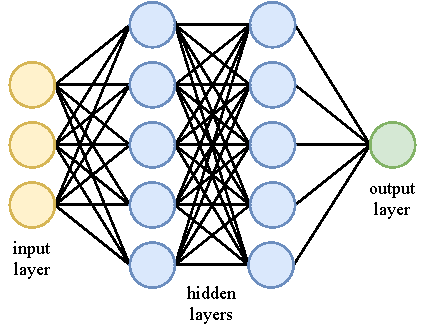
\includegraphics[width=0.6\textwidth]{diagrams/7-cvn/network.pdf}
    \caption[network short]
    {network long}
    \label{fig:network}
\end{figure}

\begin{equation} % MEAN-SQUARED ERROR LOSS EQUATION %
    E(\boldsymbol{w})=
    \frac{1}{n}\displaystyle\sum_{i=1}^{n}(y_{i}-
    \hat{y}_{i}(\boldsymbol{w}))^{2}
\end{equation}

\begin{equation} % BINARY CROSS-ENTROPY EQUATION %
    E(\boldsymbol{w})=
    -\displaystyle\sum_{i=1}^{n}y_{i}\log\hat{y}_{i}(\boldsymbol{w})+
    (1-y_{i})\log[1-\hat{y}_{i}(\boldsymbol{w})]
\end{equation}

\begin{equation} % CATEGORICAL CROSS-ENTROPY EQUATION %
    E(\boldsymbol{w})=
    -\displaystyle\sum_{i=1}^{n}\displaystyle\sum_{m=0}^{M-1}y_{im}\log\hat{y}_{im}
    (\boldsymbol{w})+(1-y_{im})\log[1-\hat{y}_{im}(\boldsymbol{w})]
\end{equation}

\subsection{Convolutional neural networks} %%%%%%%%%%%%%%%%%%%%%%%%%%%%%%%%%%%%%%%%%%%%%%%%%%%%%%%
\label{sec:cvn_theory_conv} %%%%%%%%%%%%%%%%%%%%%%%%%%%%%%%%%%%%%%%%%%%%%%%%%%%%%%%%%%%%%%%%%%%%%%

EQUATION: Back propogation equations derivation and explanation

\begin{figure} % ACTIVATIONS DIAGRAM %
    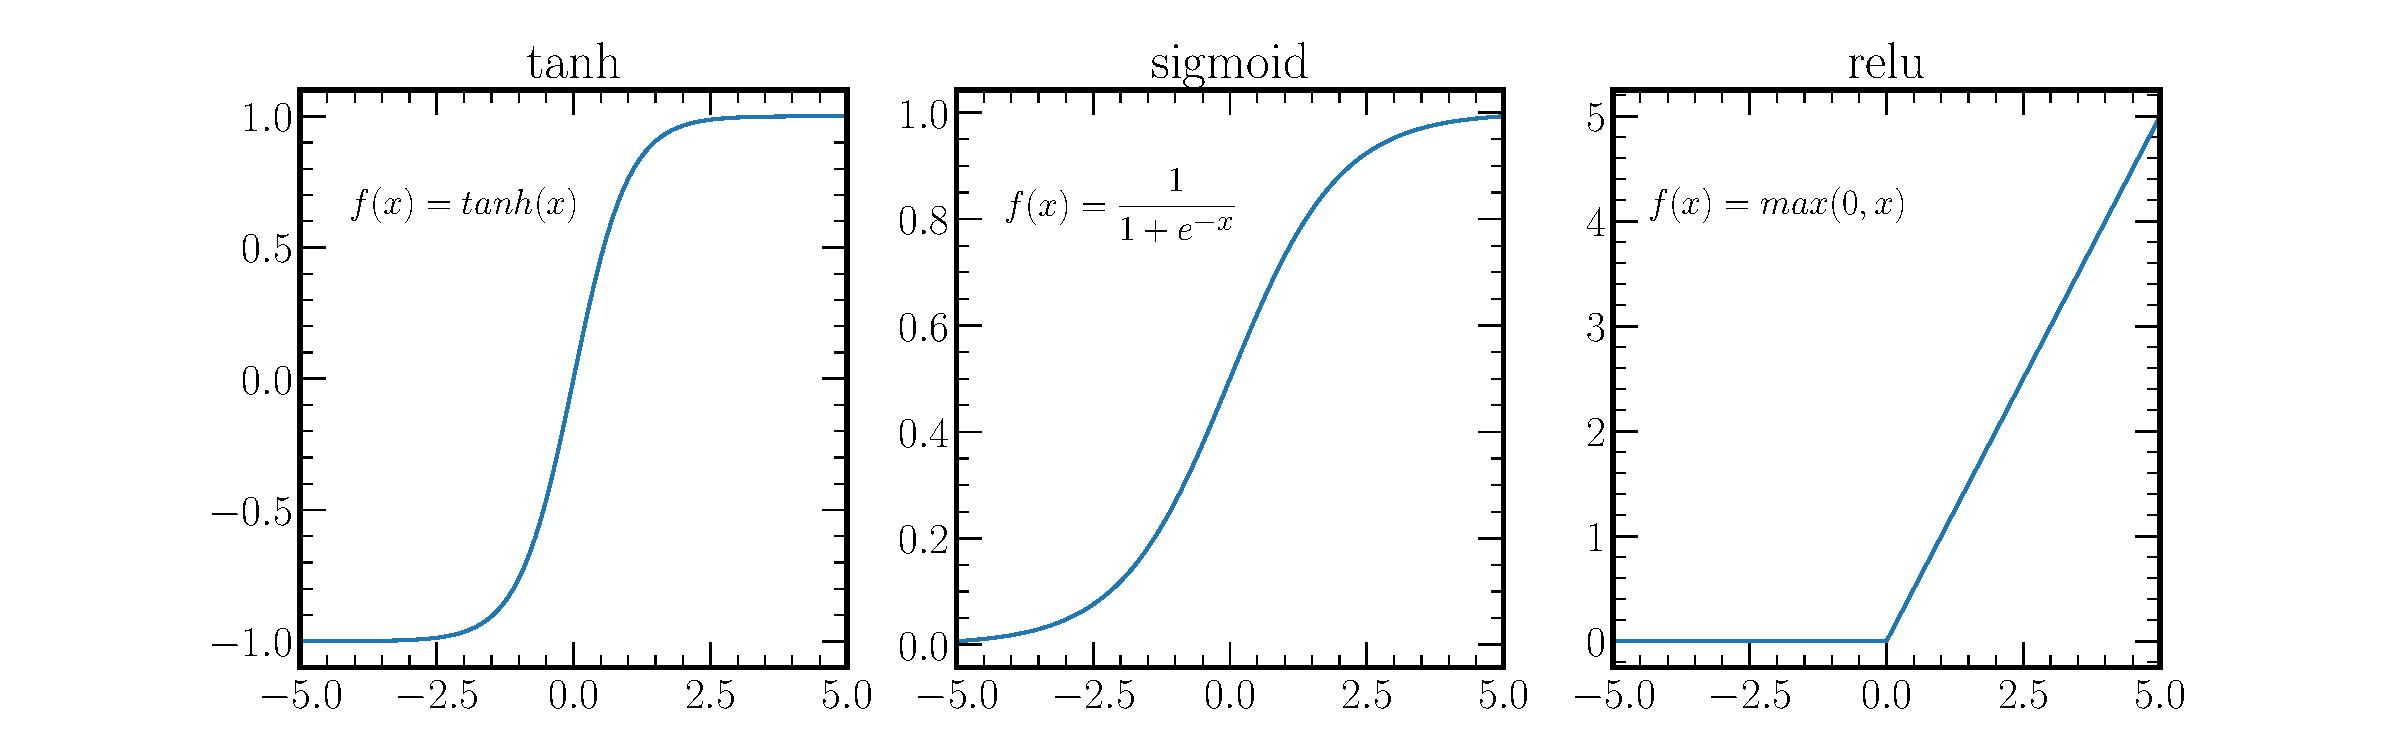
\includegraphics[width=\textwidth]{diagrams/7-cvn/activations.pdf}
    \caption[activations short]
    {activations long}
    \label{fig:activations}
\end{figure}

\begin{figure} % GRADIENT DESCENT DIAGRAM %
    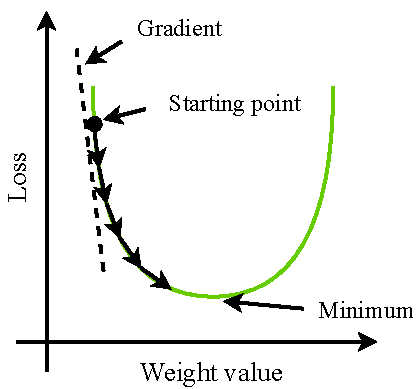
\includegraphics[width=0.5\textwidth]{diagrams/7-cvn/gradient_descent.pdf}
    \caption[gradient descent short]
    {gradient descent long}
    \label{fig:gradient_descent}
\end{figure}

\begin{figure} % CONV INPUTS DIAGRAM %
    \centering
    \begin{subfigure}[b]{0.3\textwidth}
        \centering
        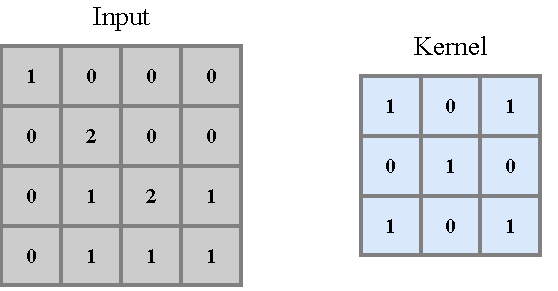
\includegraphics[width=\textwidth]{diagrams/7-cvn/conv_input.pdf}
        \caption{conv input long}
        \label{fig:conv_input}
    \end{subfigure}
    \hfill
    \begin{subfigure}[b]{0.3\textwidth}
        \centering
        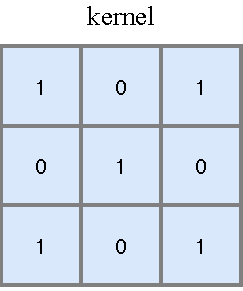
\includegraphics[width=\textwidth]{diagrams/7-cvn/conv_kernel.pdf}
        \caption{conv kernel long}
        \label{fig:conv_kernel}
    \end{subfigure}
    \caption{conv input and kernel}
    \label{fig:conv_input_kernel}
\end{figure}

TODO: combine the same and valid conv operations into the same diagram

\begin{figure} % CONV OPERATION DIAGRAM %
    \centering
    \begin{subfigure}[b]{0.71\textwidth}
        \centering
        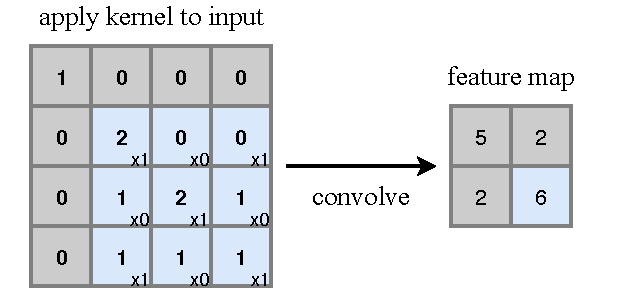
\includegraphics[width=\textwidth]{diagrams/7-cvn/conv_valid.pdf}
        \caption{conv valid long}
        \label{fig:conv_valid}
    \end{subfigure}
    \hfill
    \begin{subfigure}[b]{0.9\textwidth}
        \centering
        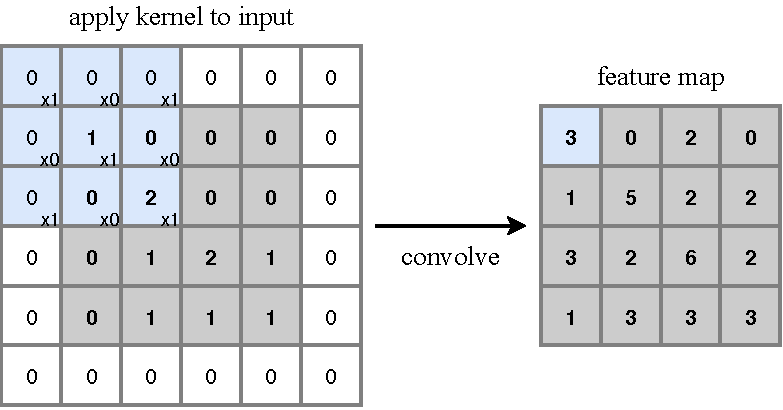
\includegraphics[width=\textwidth]{diagrams/7-cvn/conv_same.pdf}
        \caption{conv same long}
        \label{fig:conv_same}
    \end{subfigure}
    \caption{conv operations}
    \label{fig:conv_operations}
\end{figure}

\begin{figure} % POOLING DIAGRAM %
    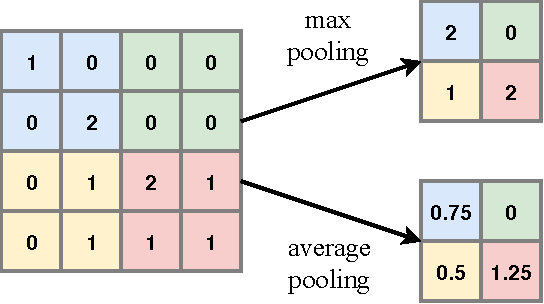
\includegraphics[width=0.6\textwidth]{diagrams/7-cvn/pooling.pdf}
    \caption[pooling short]
    {pooling long}
    \label{fig:pooling}
\end{figure}

\subsection{The evolution of convolutional networks} %%%%%%%%%%%%%%%%%%%%%%%%%%%%%%%%%%%%%%%%%%%%%
\label{sec:cvn_theory_architectures} %%%%%%%%%%%%%%%%%%%%%%%%%%%%%%%%%%%%%%%%%%%%%%%%%%%%%%%%%%%%%

Original 'dropout' paper in Ref.~\cite{hinton2012}
Original Batch normalisation paper in Ref.~\cite{ioffe2015}
Bag of tricks in Ref.~\cite{he2019}
VGG paper in Ref.~\cite{simonyan2014}
Original resnet paper in Ref.~\cite{he2016_original}
Improved resnet paper in Ref.~\cite{he2016_improved}
Inception-resnet paper in Ref.~\cite{szegedy2016}
Squeeze-and-excitation networks paper in Ref.~\cite{hu2018}
MobileNetV2 paper in Ref.~\cite{sandler2018}
EfficientNet paper in Ref.~\cite{tan2019}

EQUATION: Batch-normalisation equations

\begin{figure} % DROPOUT DIAGRAM %
    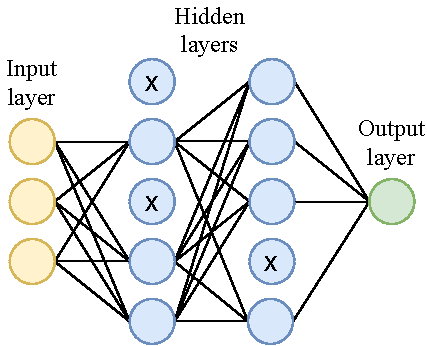
\includegraphics[width=0.6\textwidth]{diagrams/7-cvn/dropout.pdf}
    \caption[dropout short]
    {dropout long}
    \label{fig:dropout}
\end{figure}

\begin{figure} % EARLY STOPPING DIAGRAM %
    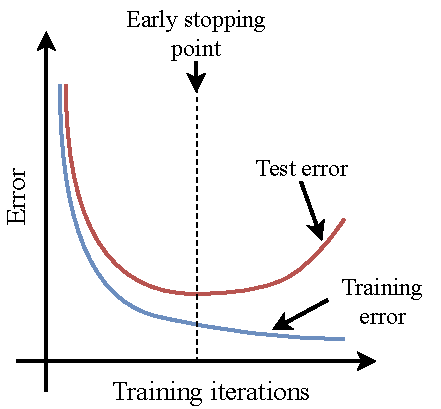
\includegraphics[width=0.5\textwidth]{diagrams/7-cvn/early_stopping.pdf}
    \caption[early stopping short]
    {early stopping long}
    \label{fig:early_stopping}
\end{figure}

\begin{figure} % SQUEEZE-EXITATION BLOCK DIAGRAM %
    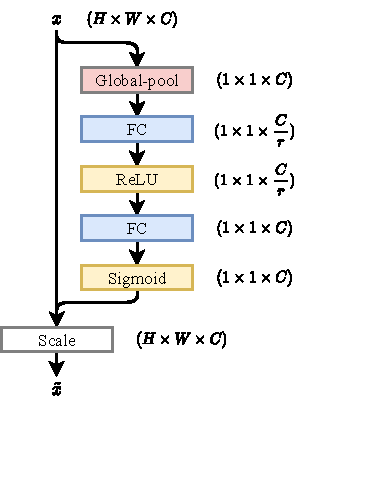
\includegraphics[width=0.5\textwidth]{diagrams/7-cvn/se.pdf}
    \caption[se short]
    {se long}
    \label{fig:se}
\end{figure}

\begin{figure} % RESNET BLOCK DIAGRAM %
    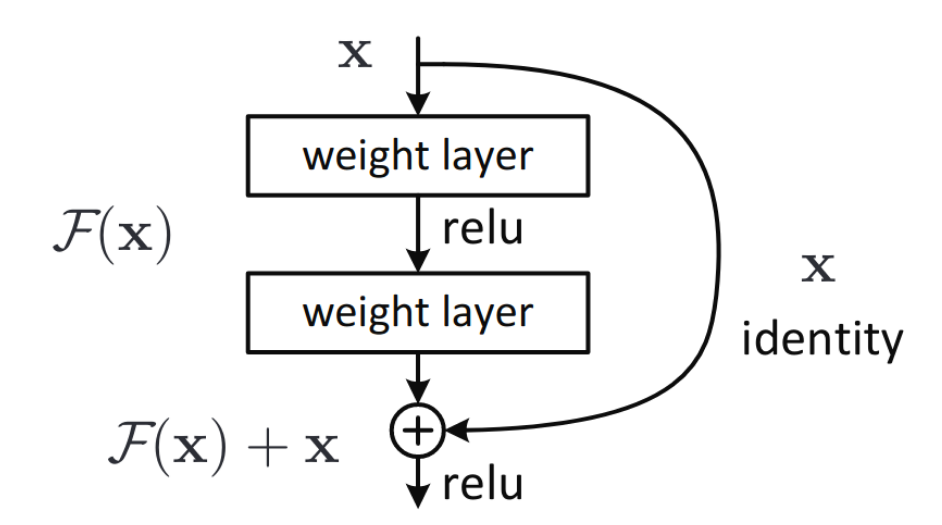
\includegraphics[width=0.6\textwidth]{diagrams/7-cvn/resnet_unit.png}
    \caption[resnet unit short]
    {resnet unit long}
    \label{fig:resnet_unit}
\end{figure}

\begin{figure} % INCEPTION BLOCK DIAGRAM %
    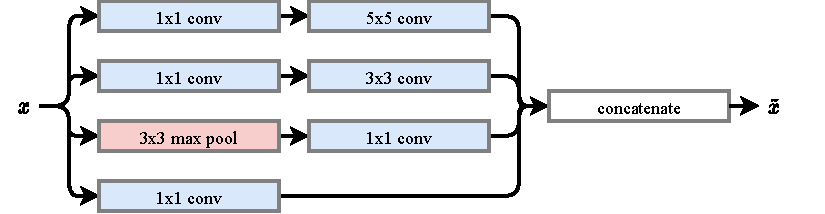
\includegraphics[width=0.8\textwidth]{diagrams/7-cvn/inception.pdf}
    \caption[inception short]
    {inception long}
    \label{fig:se}
\end{figure}

\section{A baseline implementation for CHIPS} %%%%%%%%%%%%%%%%%%%%%%%%%%%%%%%%%%%%%%%%%%%%%%%%%%%%
\label{sec:cvn_baseline} %%%%%%%%%%%%%%%%%%%%%%%%%%%%%%%%%%%%%%%%%%%%%%%%%%%%%%%%%%%%%%%%%%%%%%%%%

\begin{figure} % NU ENERGIES DIAGRAM %
    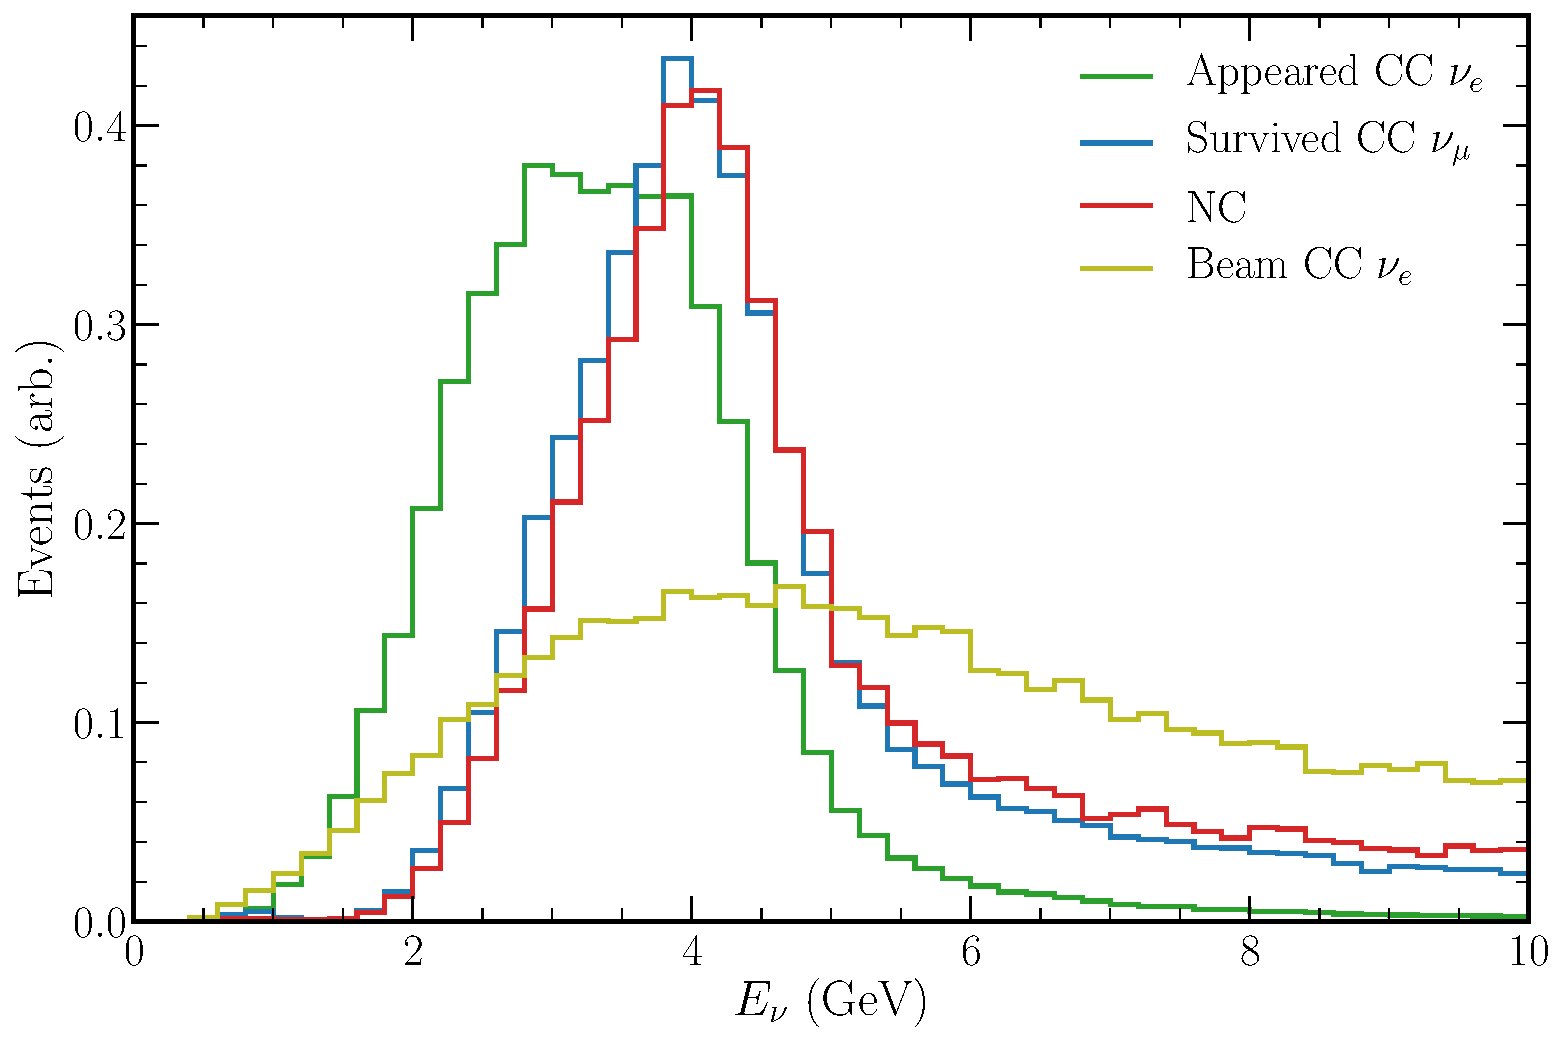
\includegraphics[width=0.6\textwidth]{diagrams/7-cvn/chipsnet/explore_nu_energies.pdf}
    \caption[explore nu energies short]
    {explore nu energies long}
    \label{fig:explore_nu_energies}
\end{figure}

\begin{figure} % OSC FLUXES DIAGRAM %
    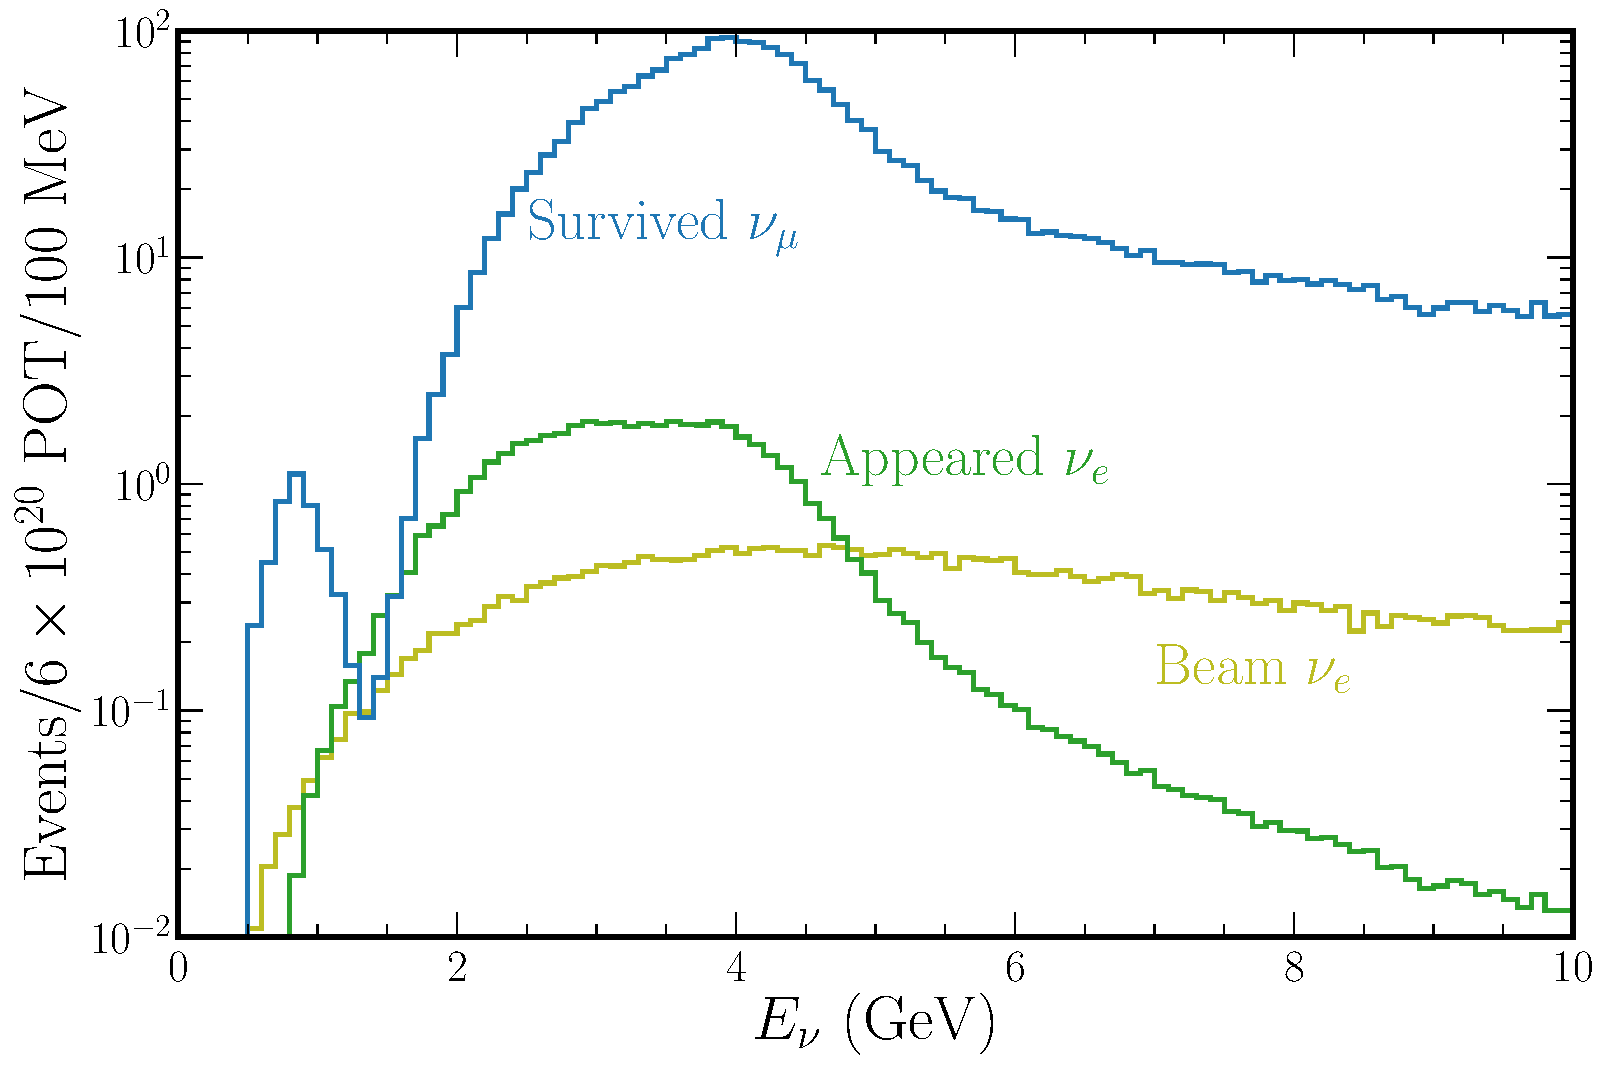
\includegraphics[width=0.6\textwidth]{diagrams/7-cvn/chipsnet/explore_osc_fluxes.pdf}
    \caption[explore osc fluxes short]
    {explore osc fluxes long}
    \label{fig:explore_osc_fluxes}
\end{figure}

\begin{figure} % SIMPLE CUTS DIAGRAM %
    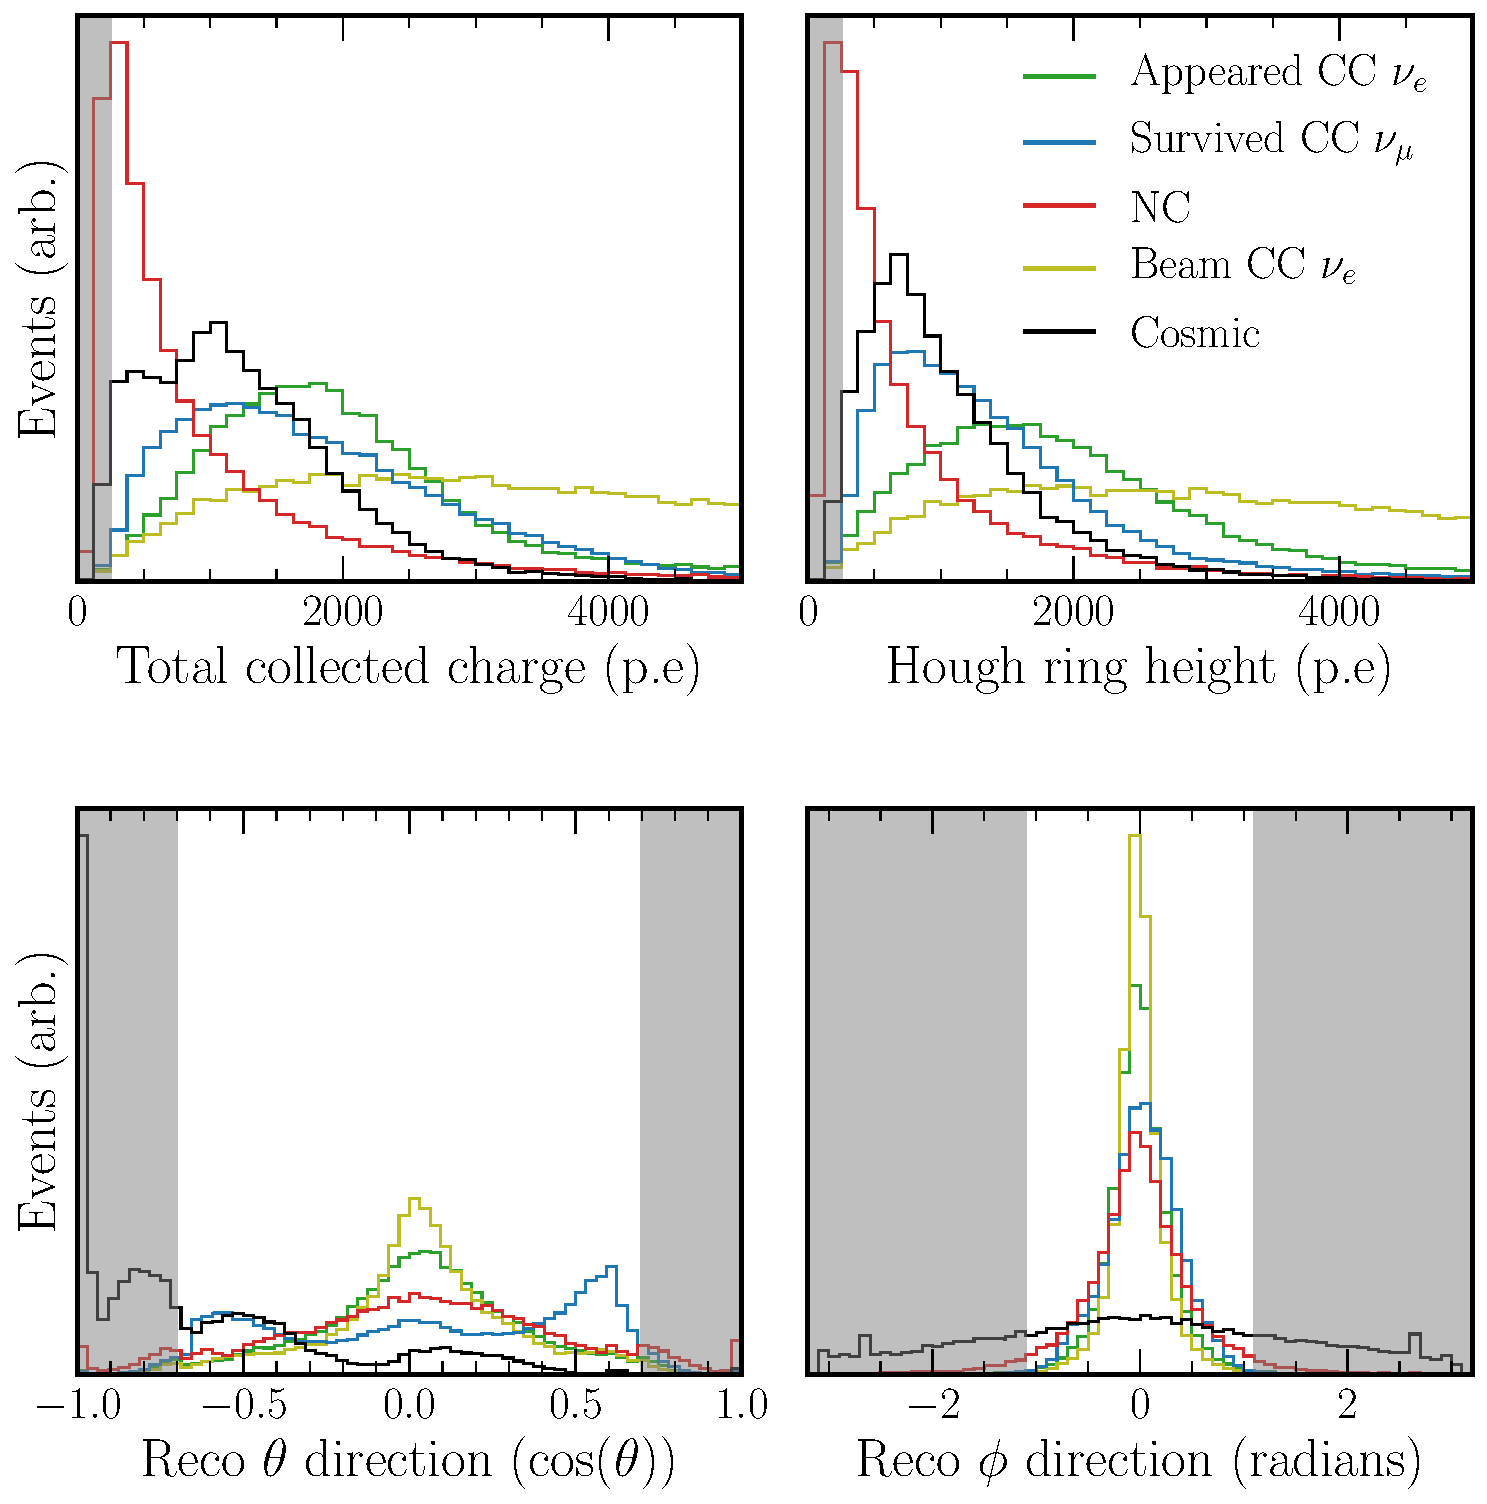
\includegraphics[width=0.8\textwidth]{diagrams/7-cvn/chipsnet/explore_simple_cuts.pdf}
    \caption[explore simple cuts short]
    {explore simple cuts long}
    \label{fig:explore_simple_cuts}
\end{figure}

\subsection{Software implementation} %%%%%%%%%%%%%%%%%%%%%%%%%%%%%%%%%%%%%%%%%%%%%%%%%%%%%%%%%%%%%
\label{sec:cvn_baseline_soft} %%%%%%%%%%%%%%%%%%%%%%%%%%%%%%%%%%%%%%%%%%%%%%%%%%%%%%%%%%%%%%%%%%%%

- Early stopping
- Model (dropout, batch norm, se, vgg etc...)

[0,25], outside range: 0.0010
    [0,120], outside range: 0.0015
    [0,3500], outside range: 0.0023

\begin{figure} % 8-BIT DIAGRAM %
    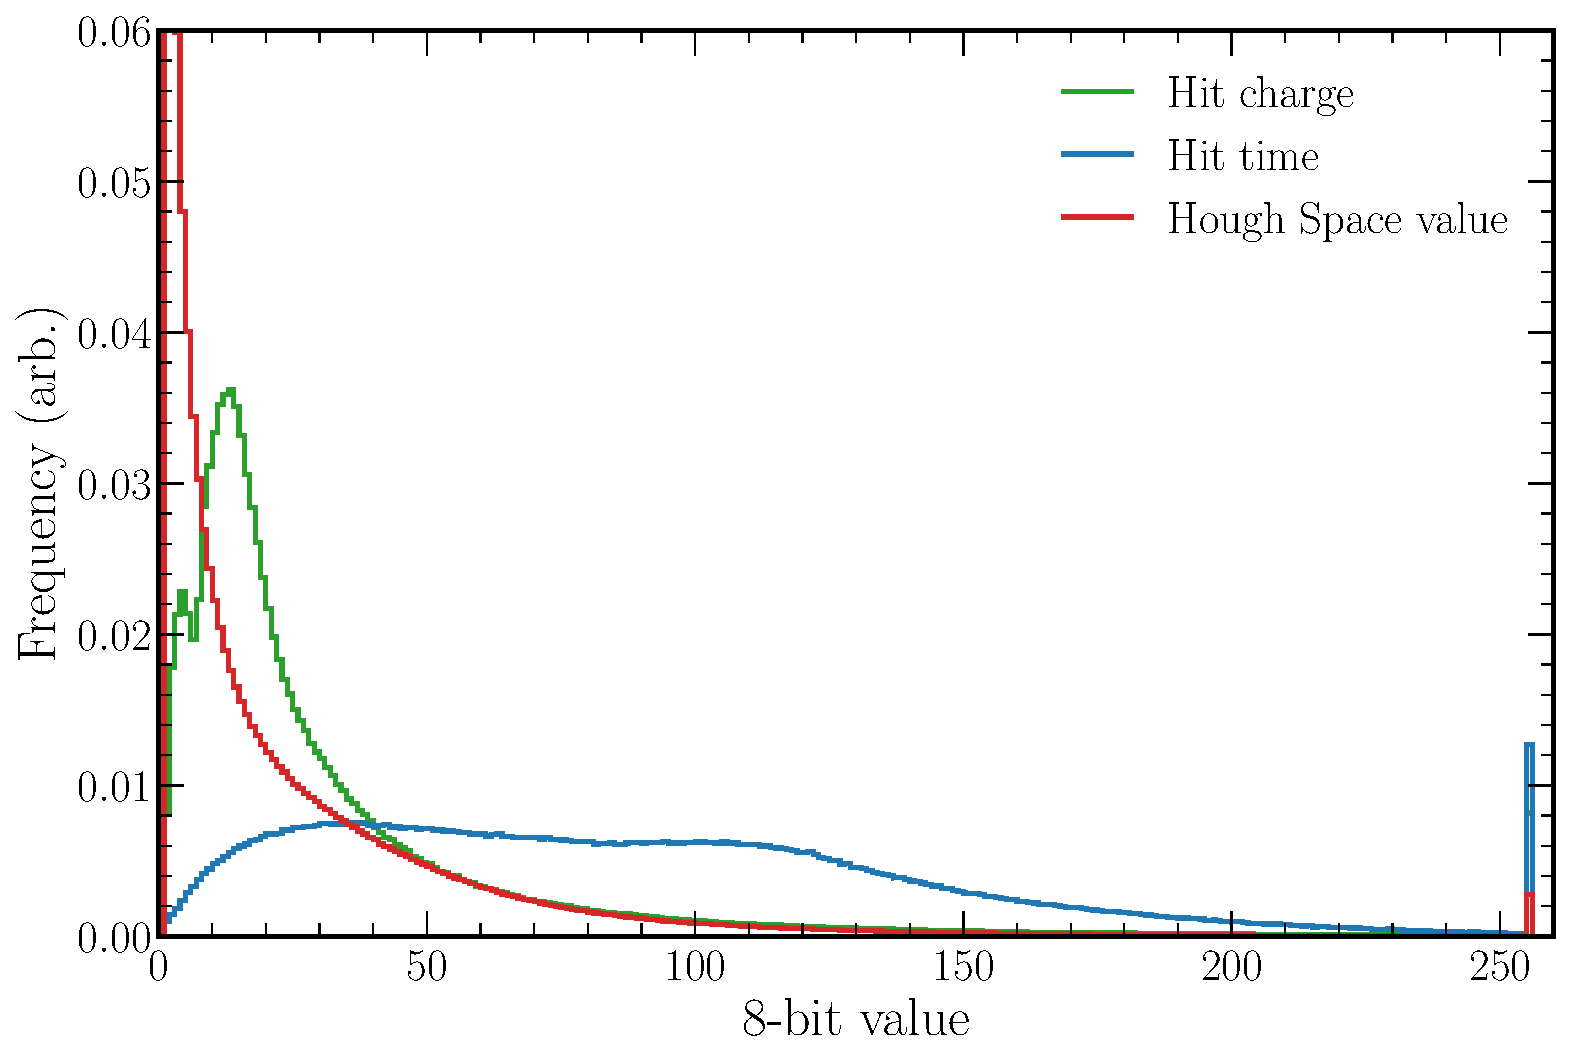
\includegraphics[width=0.6\textwidth]{diagrams/7-cvn/chipsnet/explore_8_bit_range.pdf}
    \caption[explore 8 bit range short]
    {explore 8 bit range long}
    \label{fig:explore_8_bit_range}
\end{figure}

\subsection{Network architecture} %%%%%%%%%%%%%%%%%%%%%%%%%%%%%%%%%%%%%%%%%%%%%%%%%%%%%%%%%%%%%%%%
\label{sec:cvn_baseline_architecture} %%%%%%%%%%%%%%%%%%%%%%%%%%%%%%%%%%%%%%%%%%%%%%%%%%%%%%%%%%%%

\begin{figure} % CHIPSNET DIAGRAM %
    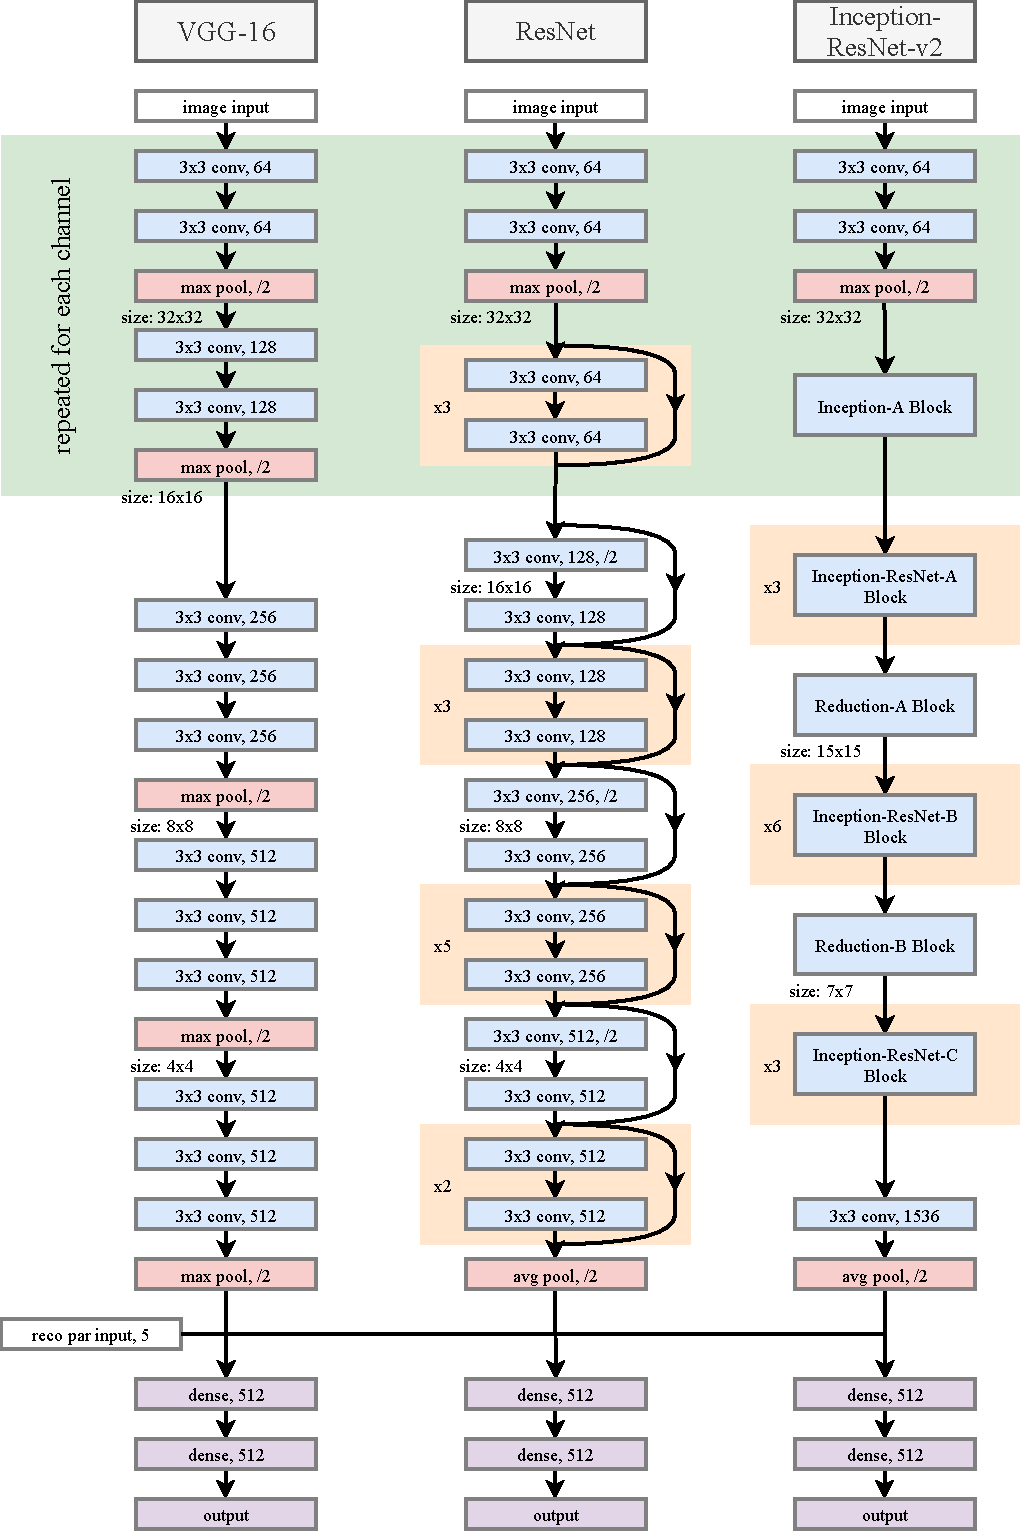
\includegraphics[width=\textwidth]{diagrams/7-cvn/chipsnet.pdf}
    \caption[chipsnet short]
    {chipsnet long}
    \label{fig:chipsnet}
\end{figure}

vgg: 17,225,296 (88ms)
inception: 16,893,216 (192ms)
resnet: 16,526,288 (112ms)
inception-resnet: 17,145,238 (209ms)

\begin{figure} % ARCHITECTURE NUEL EFF CURVES DIAGRAM %
    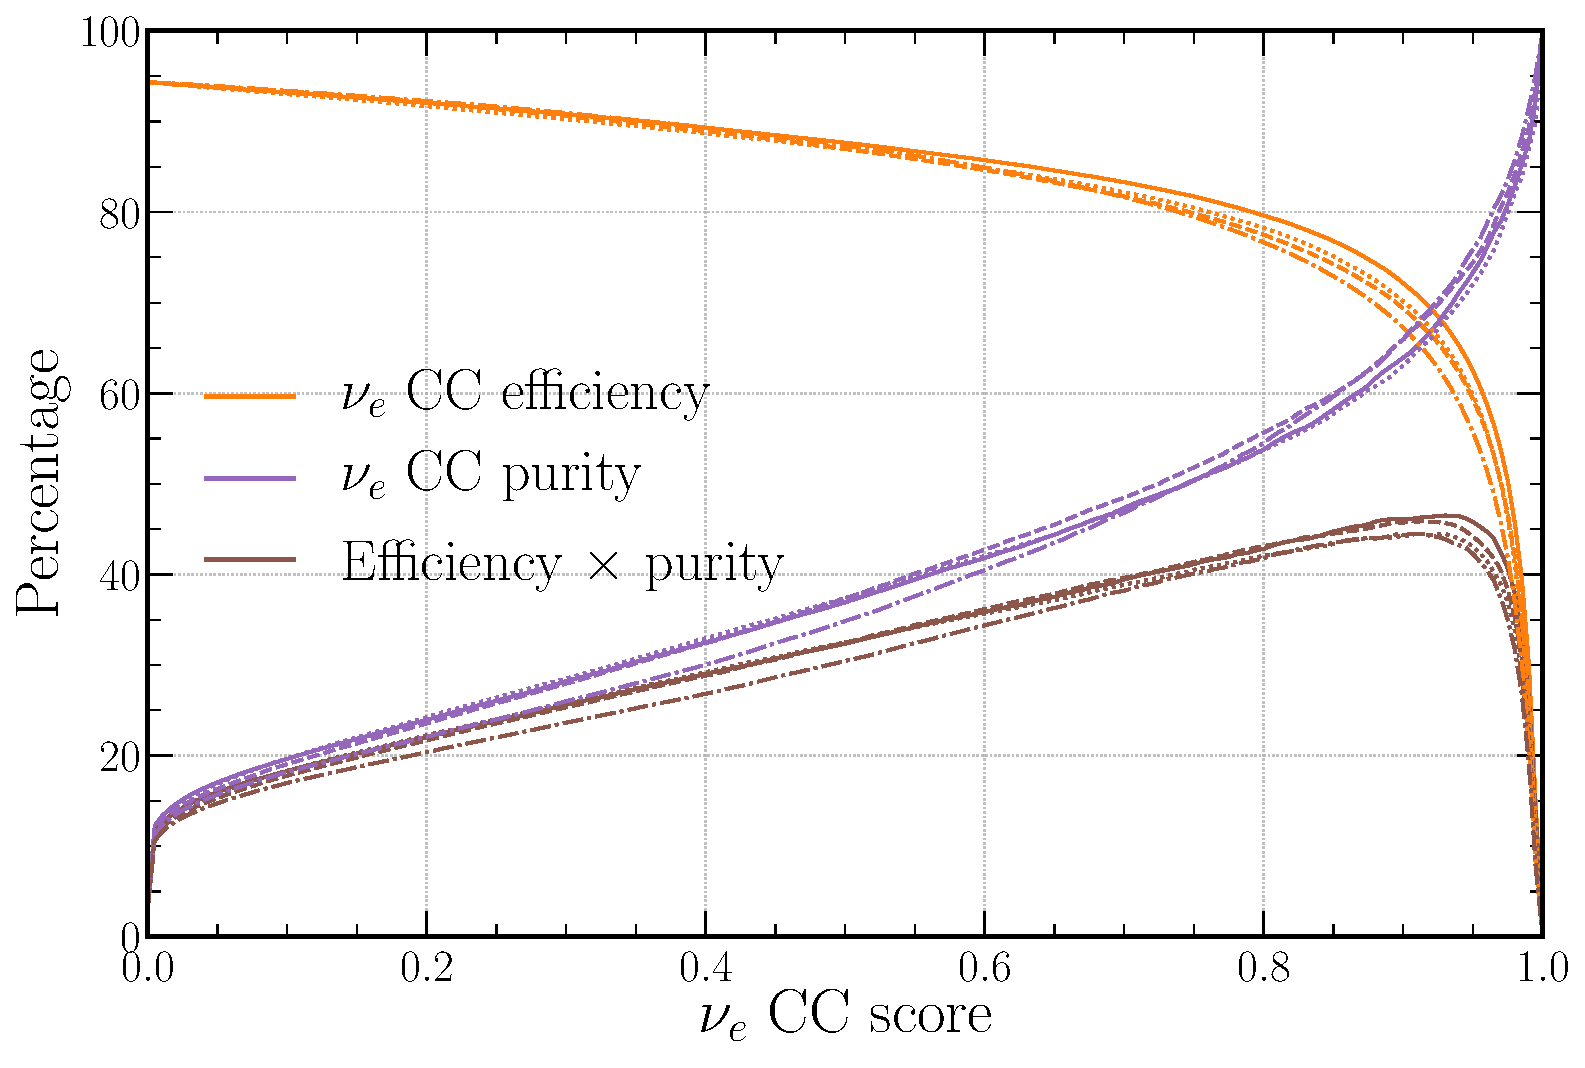
\includegraphics[width=0.6\textwidth]{diagrams/7-cvn/chipsnet/arch_nuel_eff_curves.pdf}
    \caption[arch nuel eff curves short]
    {vgg=solid, inception=dashed, resnet=dotted, inception-resnet=dot-dash}
    \label{fig:arch_nuel_eff_curves}
\end{figure}

\begin{figure} % ARCHITECTURE NUEL COMP CURVES DIAGRAM %
    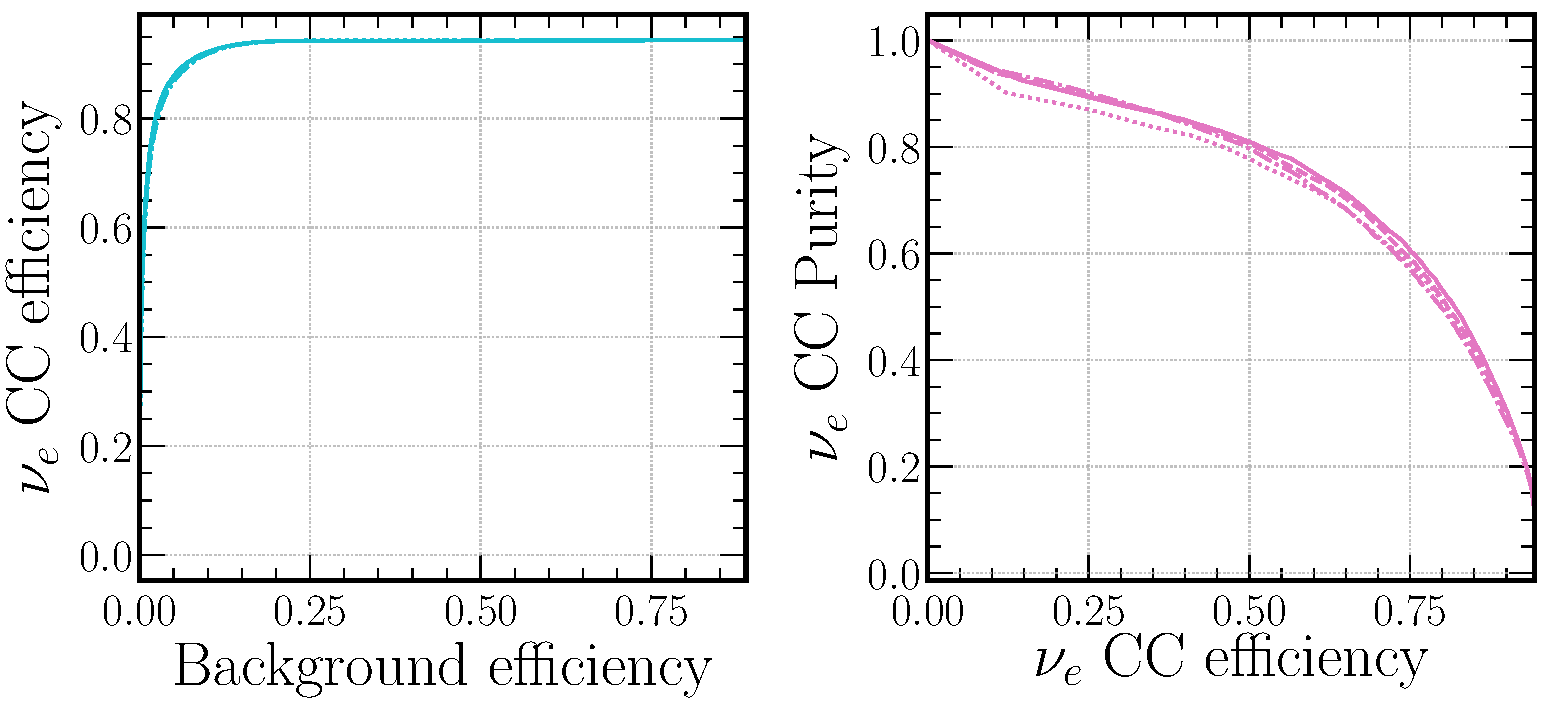
\includegraphics[width=0.8\textwidth]{diagrams/7-cvn/chipsnet/arch_nuel_comp_curves.pdf}
    \caption[arch nuel comp curves short]
    {vgg=solid, inception=dashed, resnet=dotted, inception-resnet=dot-dash}
    \label{fig:arch_nuel_comp_curves}
\end{figure}

- Nuel-> ROC-AUC: 0.82559, PRC-AUC: 0.71155, S-Eff: 0.87661, S-Pur: 0.36928
- FOM1-> 0.46510, 0.93000, 53.44422, 8.34671, 15.75487, 0.67485, 0.68920
- FOM2-> 13.44645, 0.98500, 31.21664, 1.57028, 3.81933, 0.39418, 0.85277

- Nuel-> ROC-AUC: 0.82519, PRC-AUC: 0.70632, S-Eff: 0.86992, S-Pur: 0.37332
- FOM1-> 0.45910, 0.91500, 53.20954, 9.73154, 14.92970, 0.67188, 0.68331
- FOM2-> 13.47965, 0.98500, 28.04995, 1.43802, 2.89217, 0.35419, 0.86627

- Nuel-> ROC-AUC: 0.82444, PRC-AUC: 0.68789, S-Eff: 0.86926, S-Pur: 0.37417
- FOM1-> 0.44511, 0.91000, 54.46409, 11.50537, 18.18029, 0.68772, 0.64723
- FOM2-> 12.22026, 0.98000, 32.56108, 2.77151, 4.32813, 0.41115, 0.82099

- Nuel-> ROC-AUC: 0.82444, PRC-AUC: 0.69946, S-Eff: 0.87369, S-Pur: 0.34882
- FOM1-> 0.44448, 0.90500, 52.61119, 10.90981, 15.11323, 0.66433, 0.66906
- FOM2-> 13.48962, 0.98500, 23.98040, 0.96809, 2.19211, 0.30280, 0.88356

\begin{figure} % ARCHITECTURE NUMU EFF CURVES DIAGRAM %
    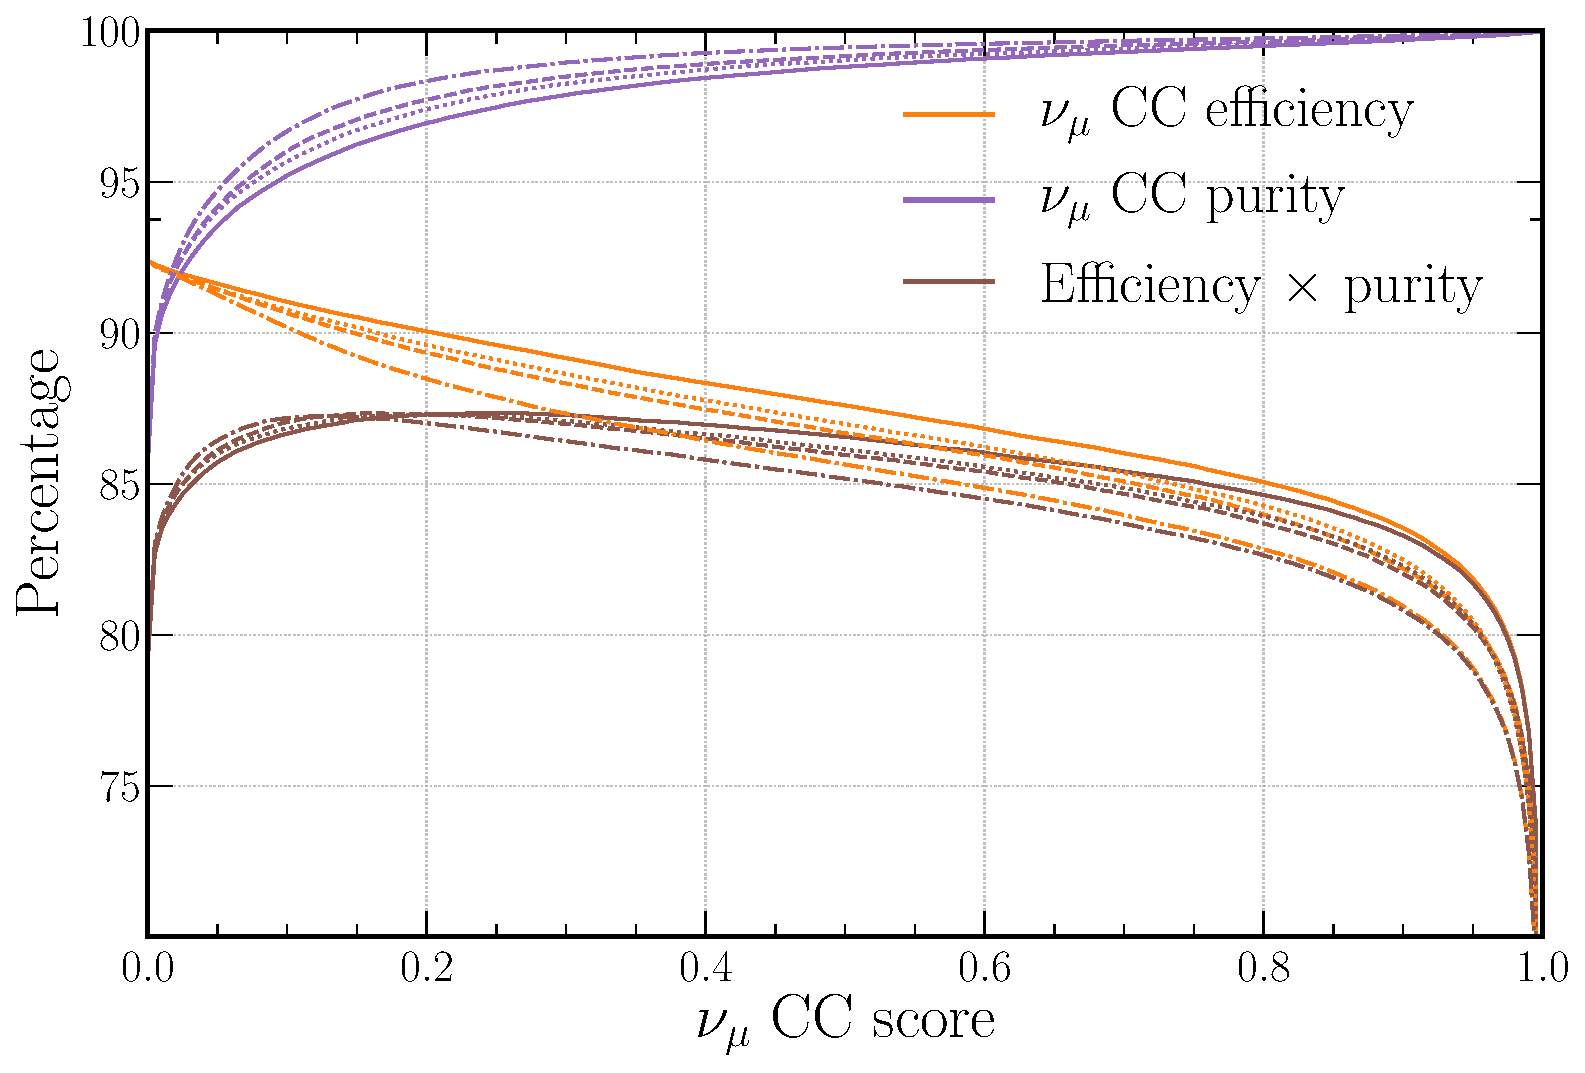
\includegraphics[width=0.6\textwidth]{diagrams/7-cvn/chipsnet/arch_numu_eff_curves.pdf}
    \caption[arch numu eff curves short]
    {vgg=solid, inception=dashed, resnet=dotted, inception-resnet=dot-dash}
    \label{fig:arch_numu_eff_curves}
\end{figure}

\begin{figure} % ARCHITECTURE NUMU COMP CURVES DIAGRAM %
    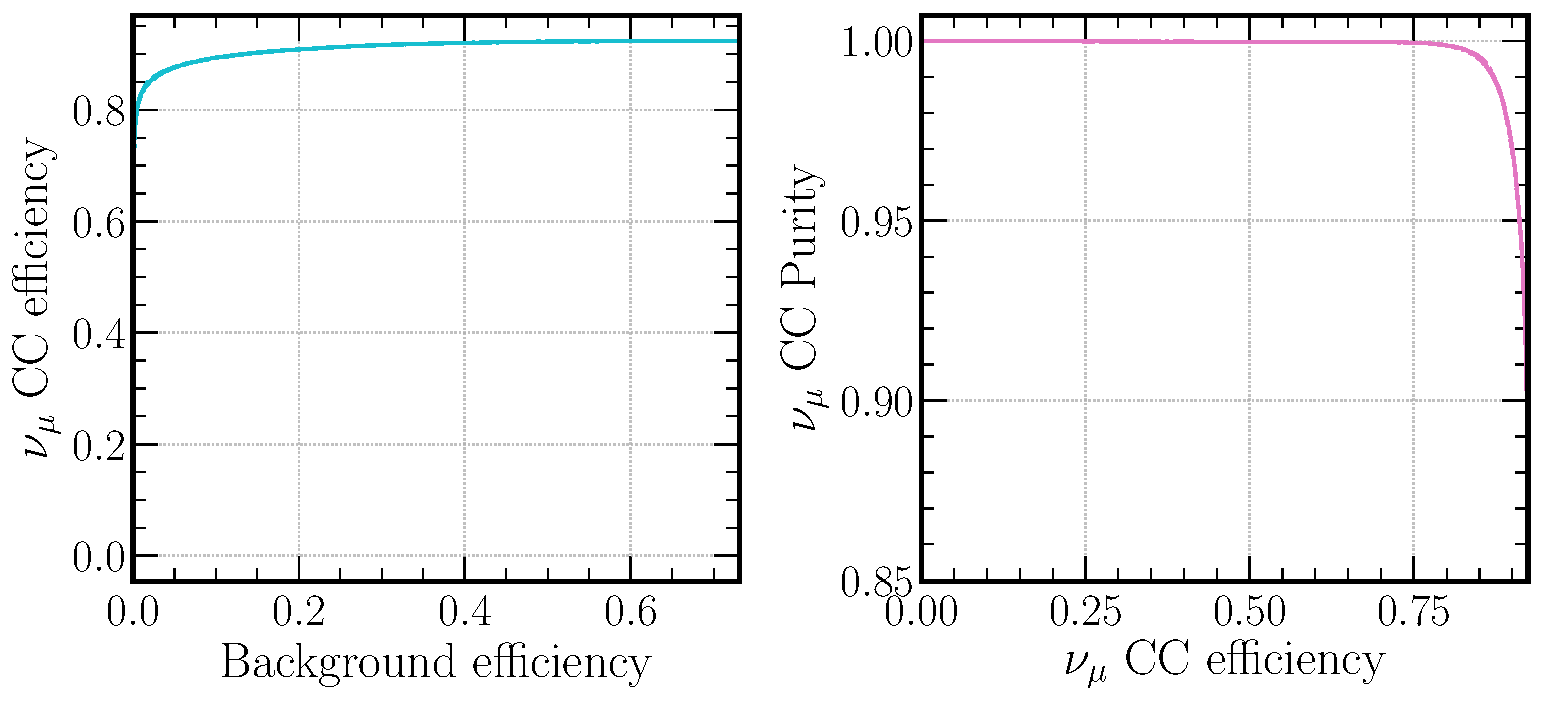
\includegraphics[width=0.8\textwidth]{diagrams/7-cvn/chipsnet/arch_numu_comp_curves.pdf}
    \caption[arch numu comp curves short]
    {vgg=solid, inception=dashed, resnet=dotted, inception-resnet=dot-dash}
    \label{fig:arch_numu_comp_curves}
\end{figure}

\subsection{Which training sample to use} %%%%%%%%%%%%%%%%%%%%%%%%%%%%%%%%%%%%%%%%%%%%%%%%%%%%%%%%
\label{sec:cvn_baseline_sample} %%%%%%%%%%%%%%%%%%%%%%%%%%%%%%%%%%%%%%%%%%%%%%%%%%%%%%%%%%%%%%%%%%

\begin{figure} % FLUX TRAINING SAMPLE DIAGRAM %
    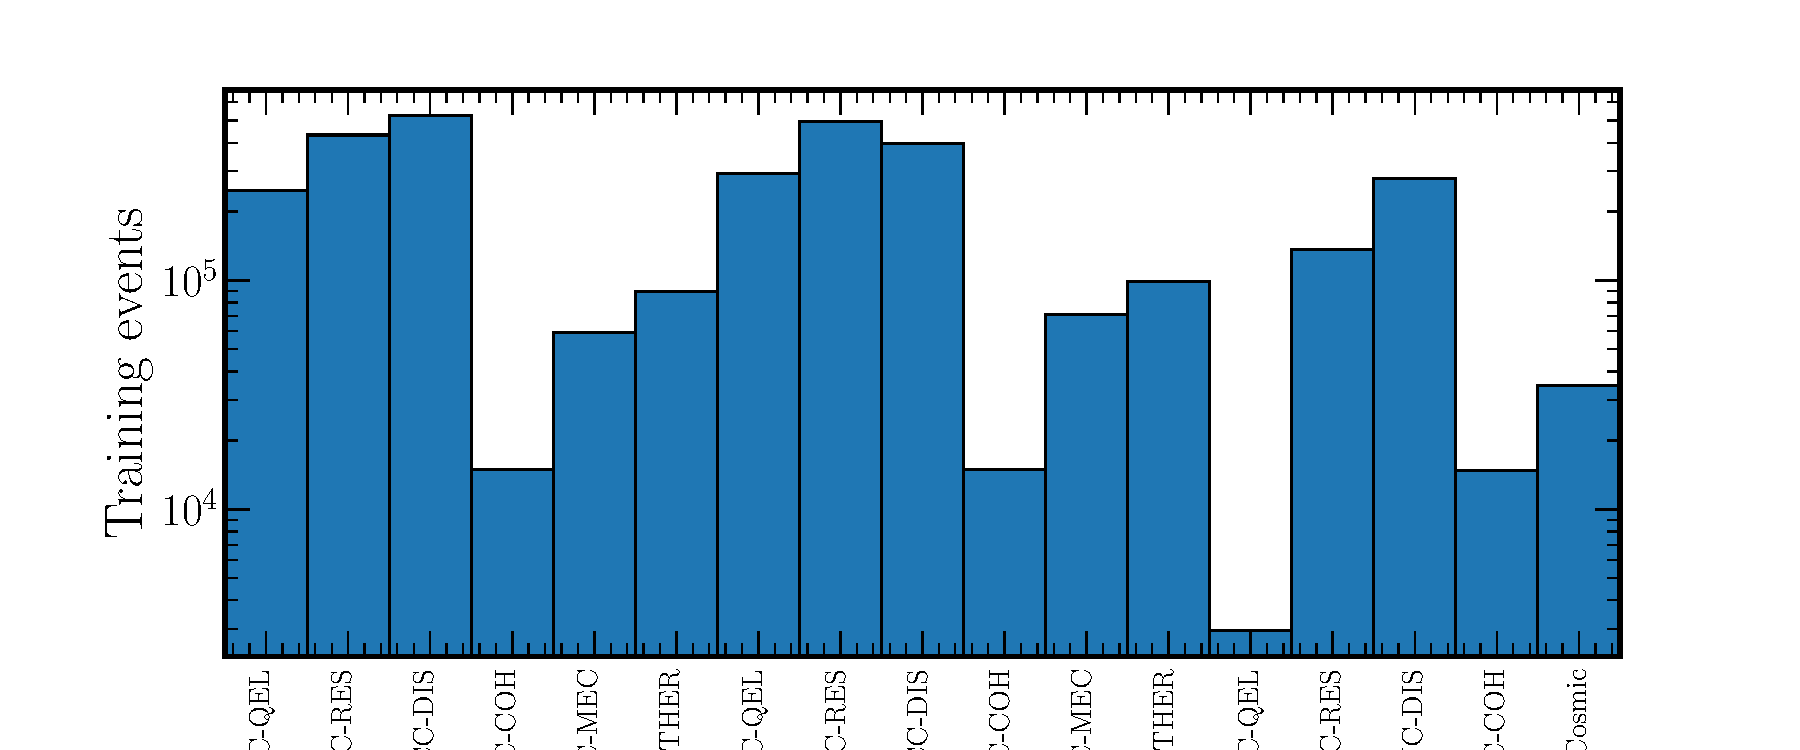
\includegraphics[width=0.6\textwidth]{diagrams/7-cvn/chipsnet/explore_flux_sample.pdf}
    \caption[explore flux sample short]
    {explore flux sample long}
    \label{fig:explore_flux_sample}
\end{figure}

\begin{figure} % UNIFORM TRAINING SAMPLE DIAGRAM %
    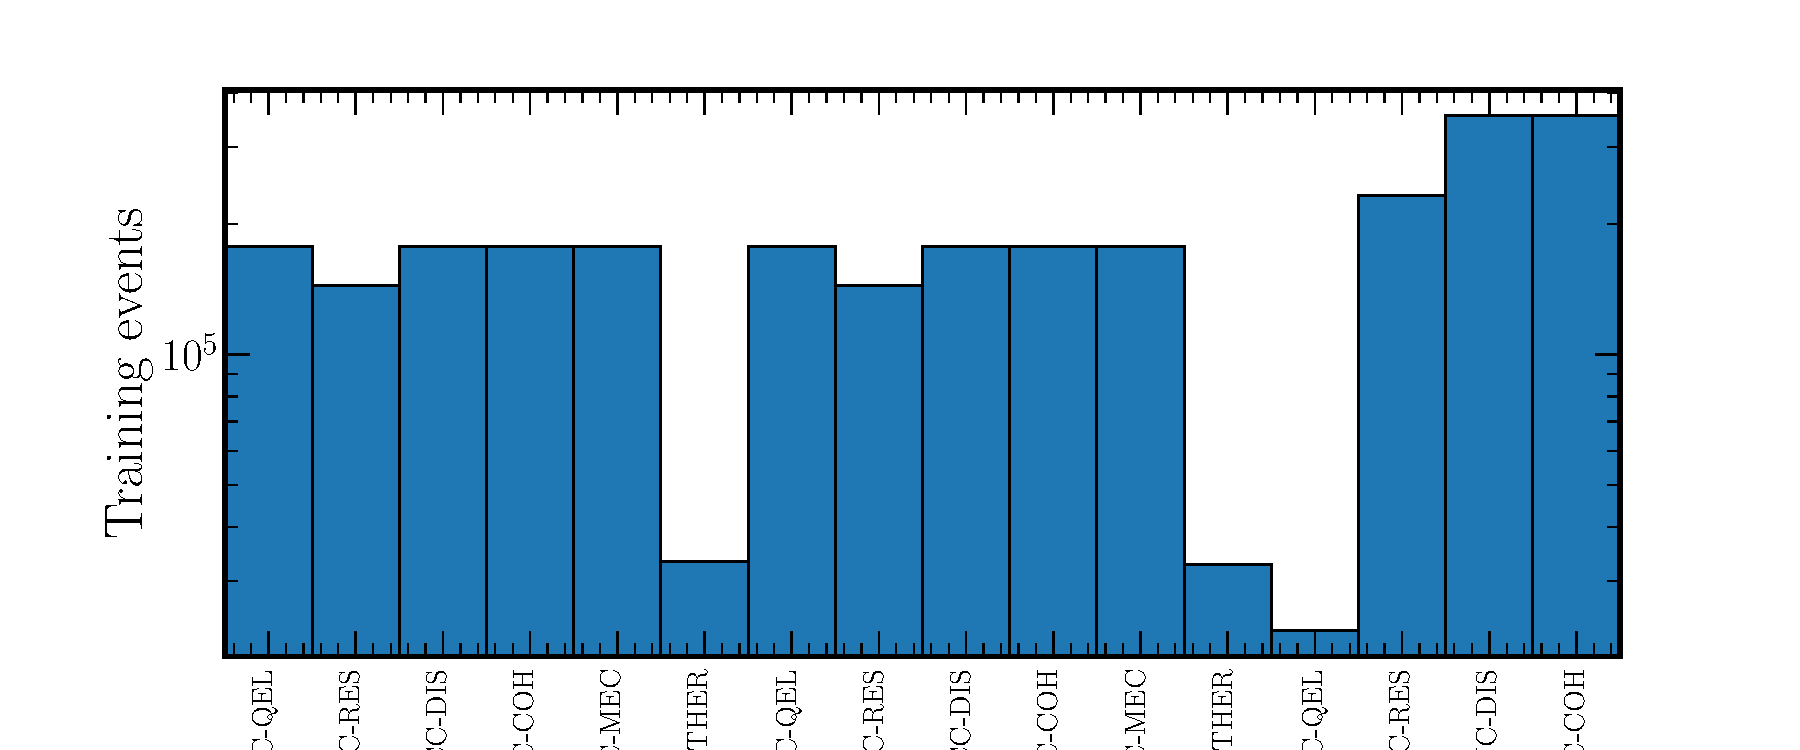
\includegraphics[width=0.6\textwidth]{diagrams/7-cvn/chipsnet/explore_uniform_sample.pdf}
    \caption[explore uniform sample short]
    {explore uniform sample long}
    \label{fig:explore_uniform_sample}
\end{figure}

\begin{figure} % BOTH TRAINING SAMPLE DIAGRAM %
    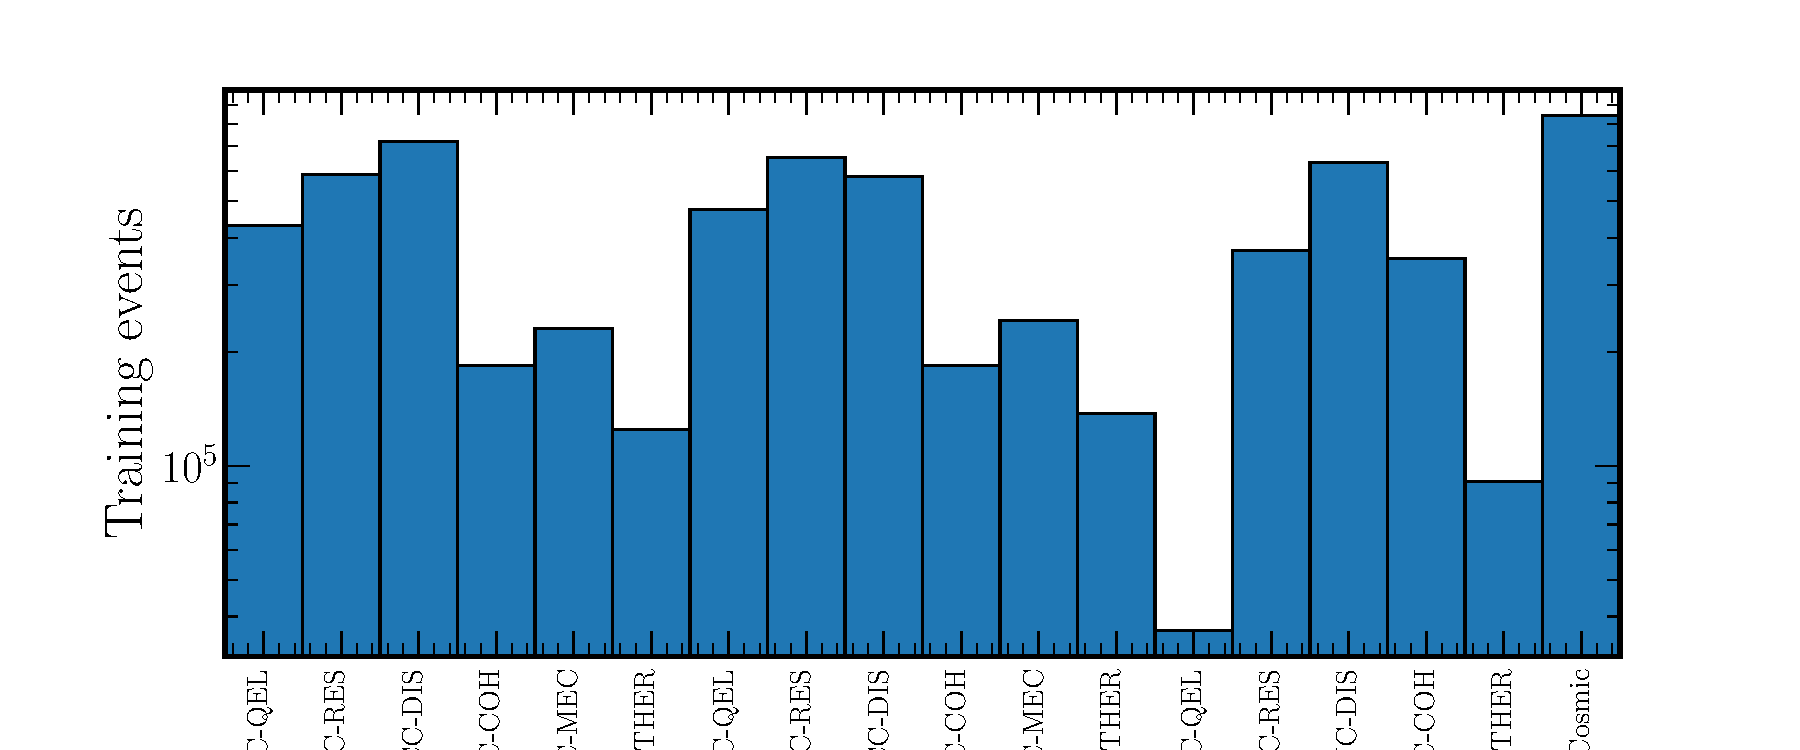
\includegraphics[width=0.6\textwidth]{diagrams/7-cvn/chipsnet/explore_both_sample.pdf}
    \caption[explore both sample short]
    {explore both sample long}
    \label{fig:explore_both_sample}
\end{figure}

\begin{figure} % SAMPLE FLUX OUTPUT DIAGRAM %
    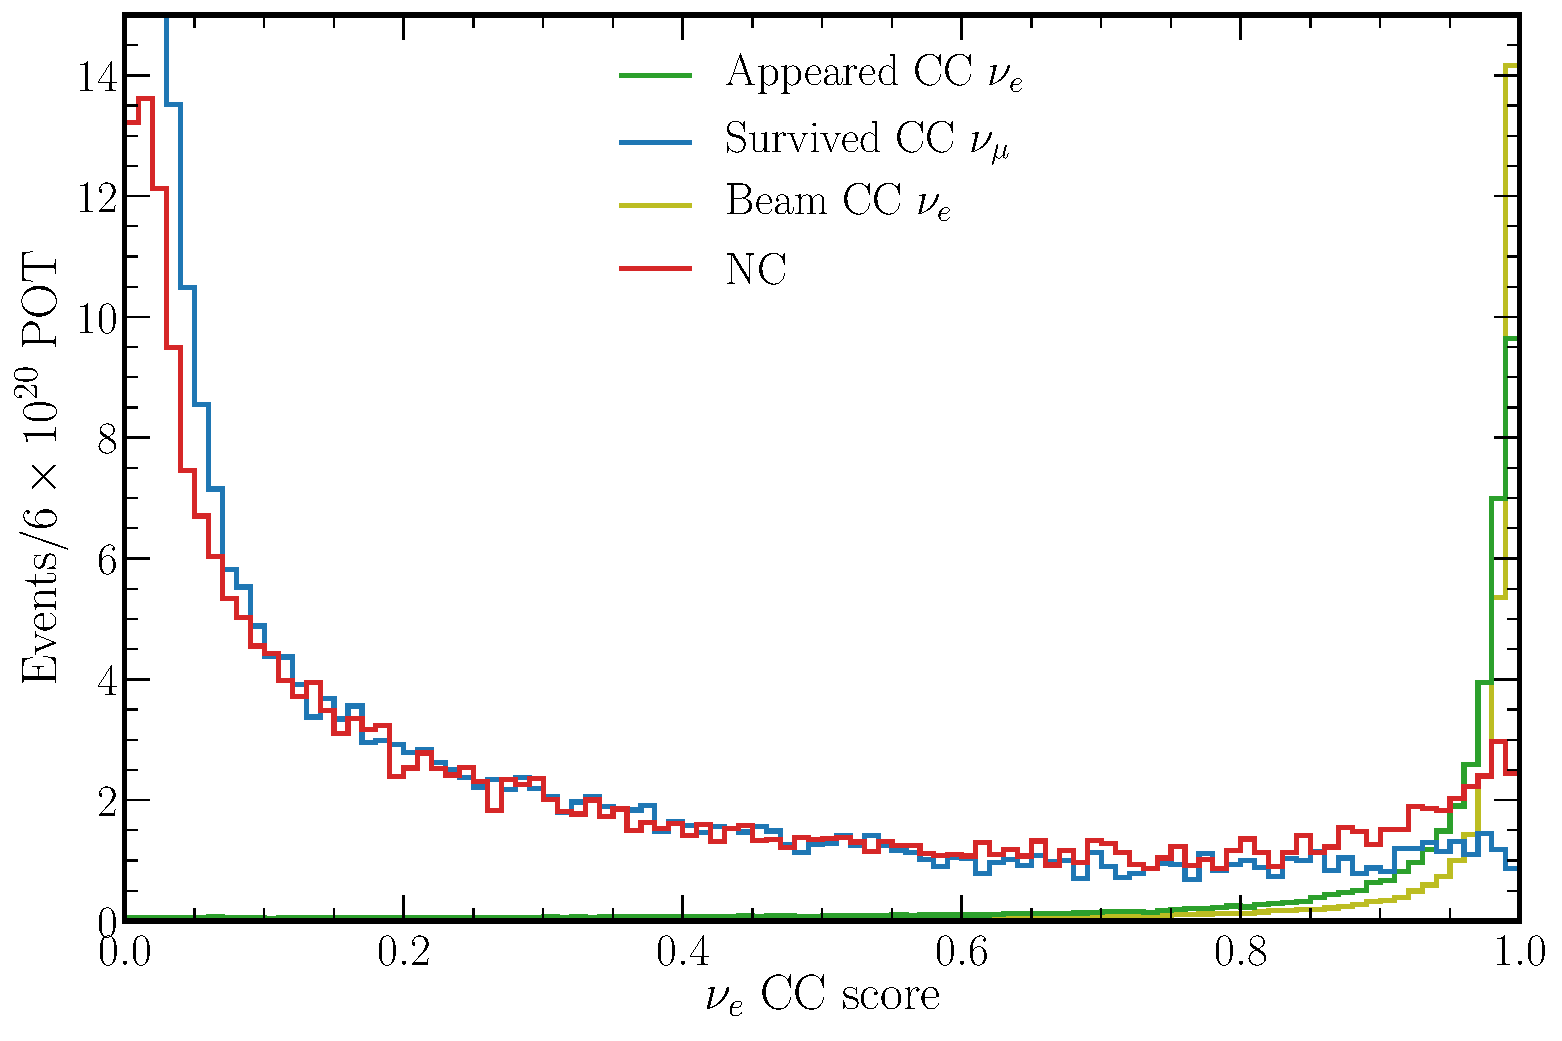
\includegraphics[width=0.6\textwidth]{diagrams/7-cvn/chipsnet/sample_flux_output_values.pdf}
    \caption[sample flux output values short]
    {sample flux output values long}
    \label{fig:sample_flux_output_values}
\end{figure}

\begin{figure} % SAMPLE UNIFORM OUTPUT DIAGRAM %
    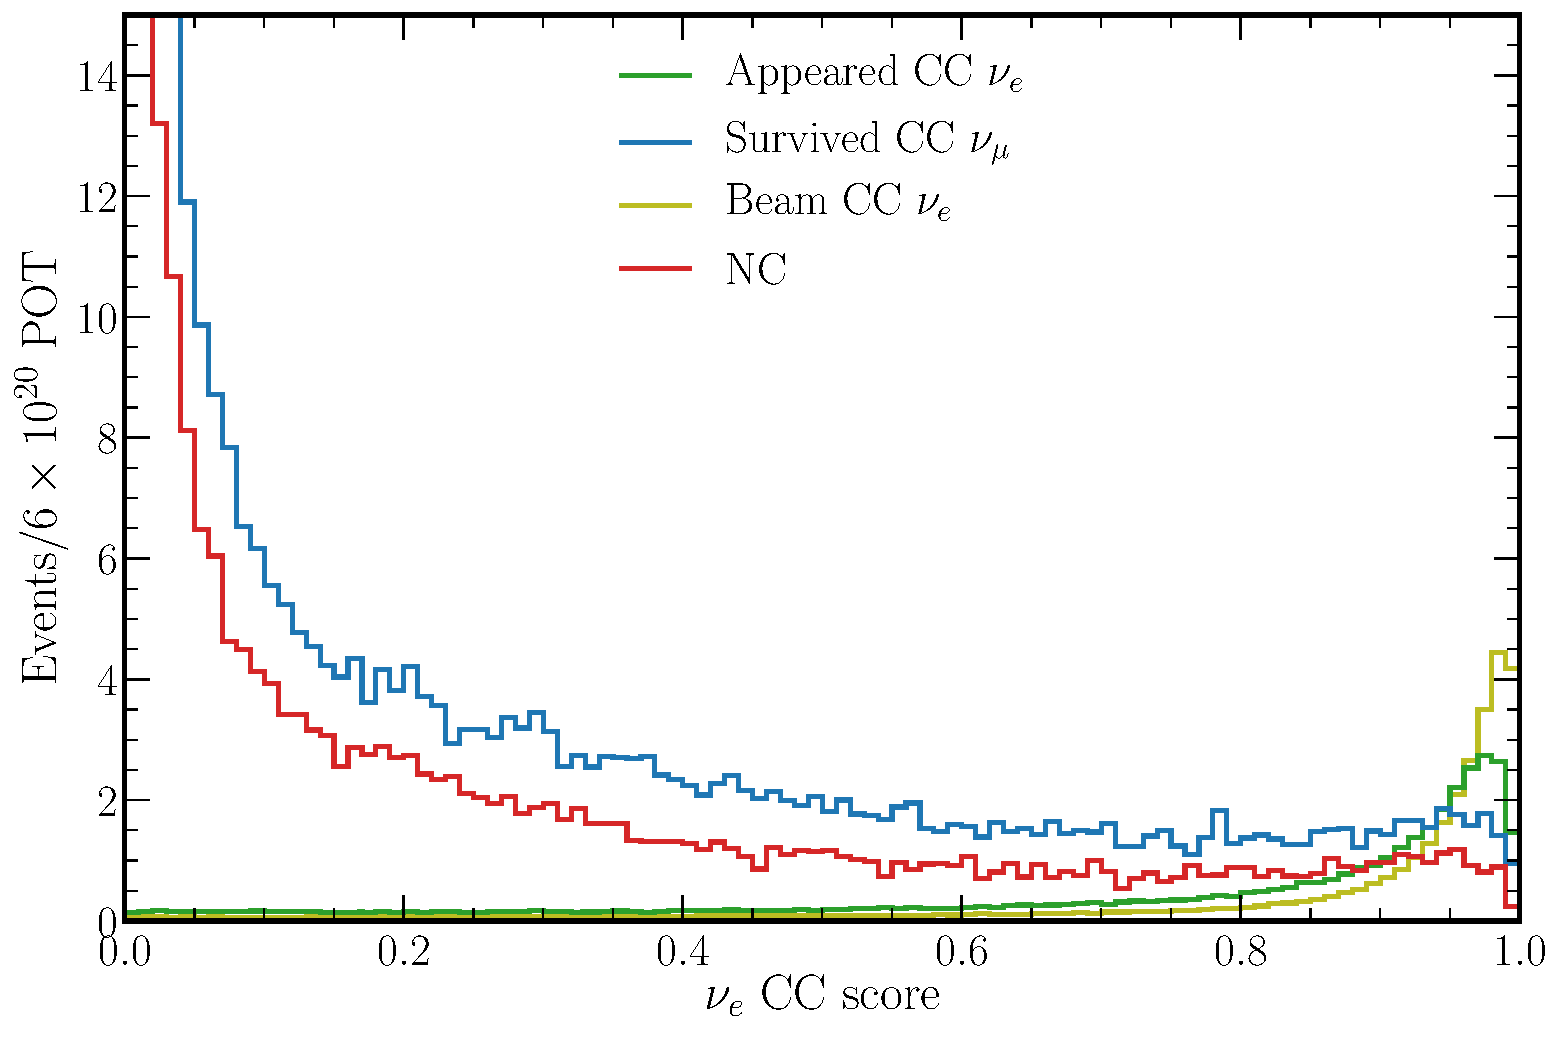
\includegraphics[width=0.6\textwidth]{diagrams/7-cvn/chipsnet/sample_uniform_output_values.pdf}
    \caption[sample uniform output values short]
    {sample uniform output values long}
    \label{fig:sample_uniform_output_values}
\end{figure}

\begin{figure} % SAMPLE BOTH OUTPUT DIAGRAM %
    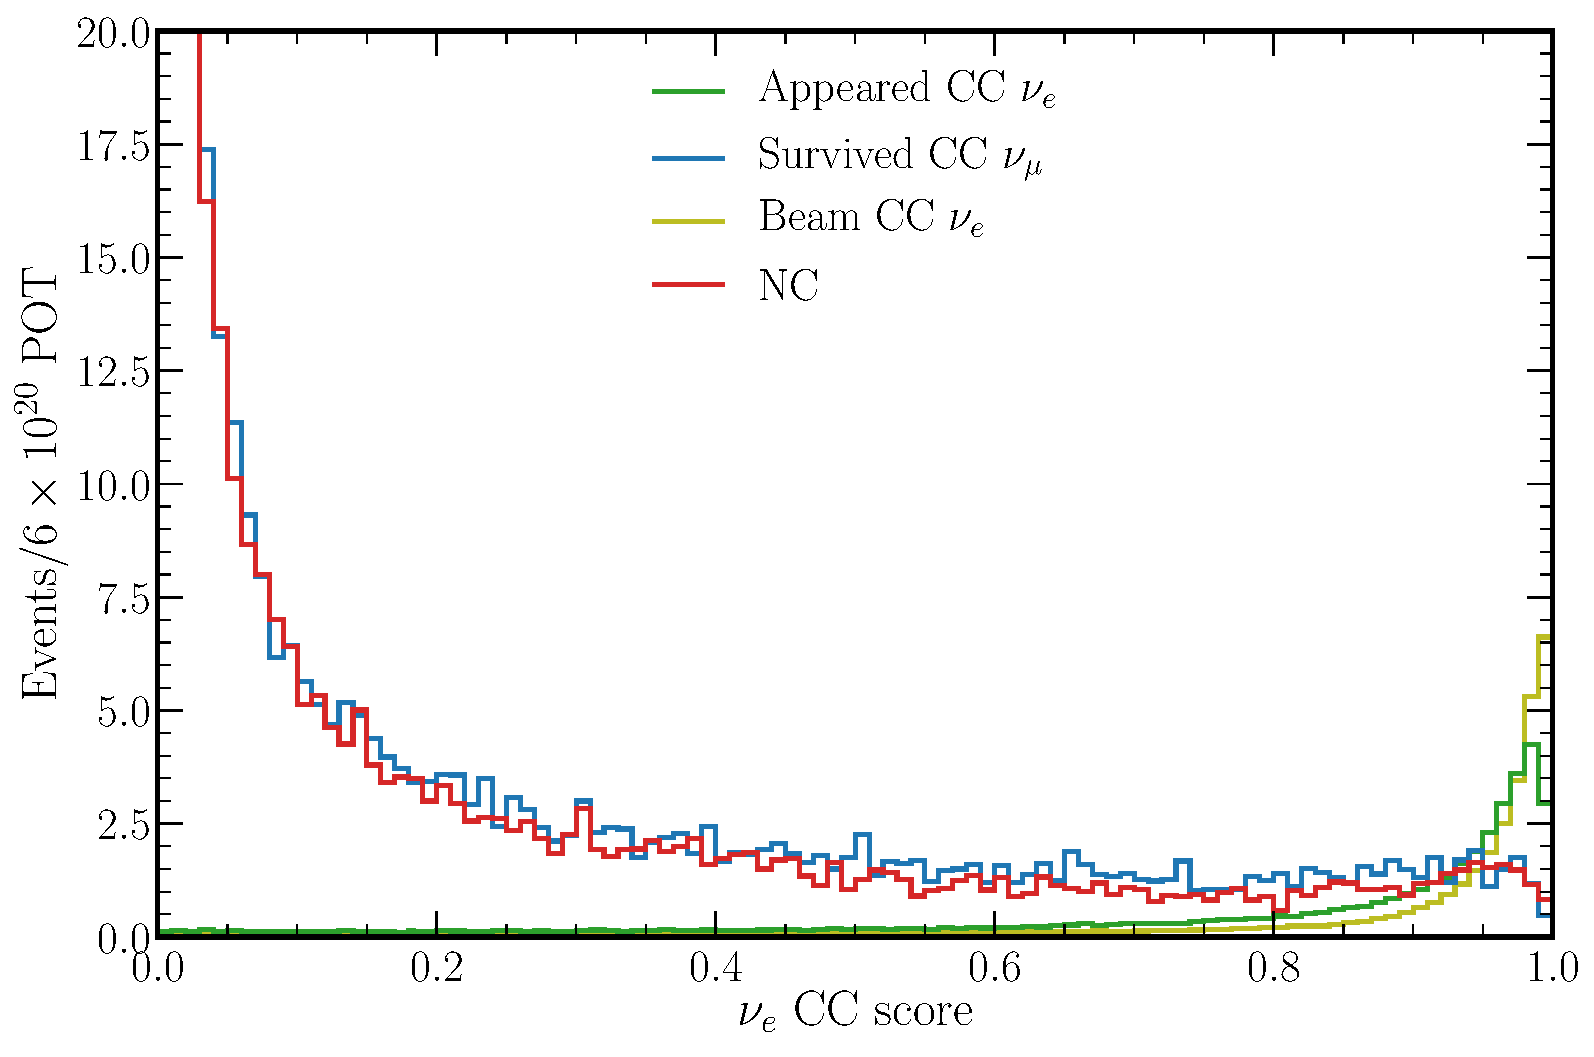
\includegraphics[width=0.6\textwidth]{diagrams/7-cvn/chipsnet/sample_both_output_values.pdf}
    \caption[sample both output values short]
    {sample both output values long}
    \label{fig:sample_both_output_values}
\end{figure}

\begin{figure} % SAMPLE NUEL EFF CURVES DIAGRAM %
    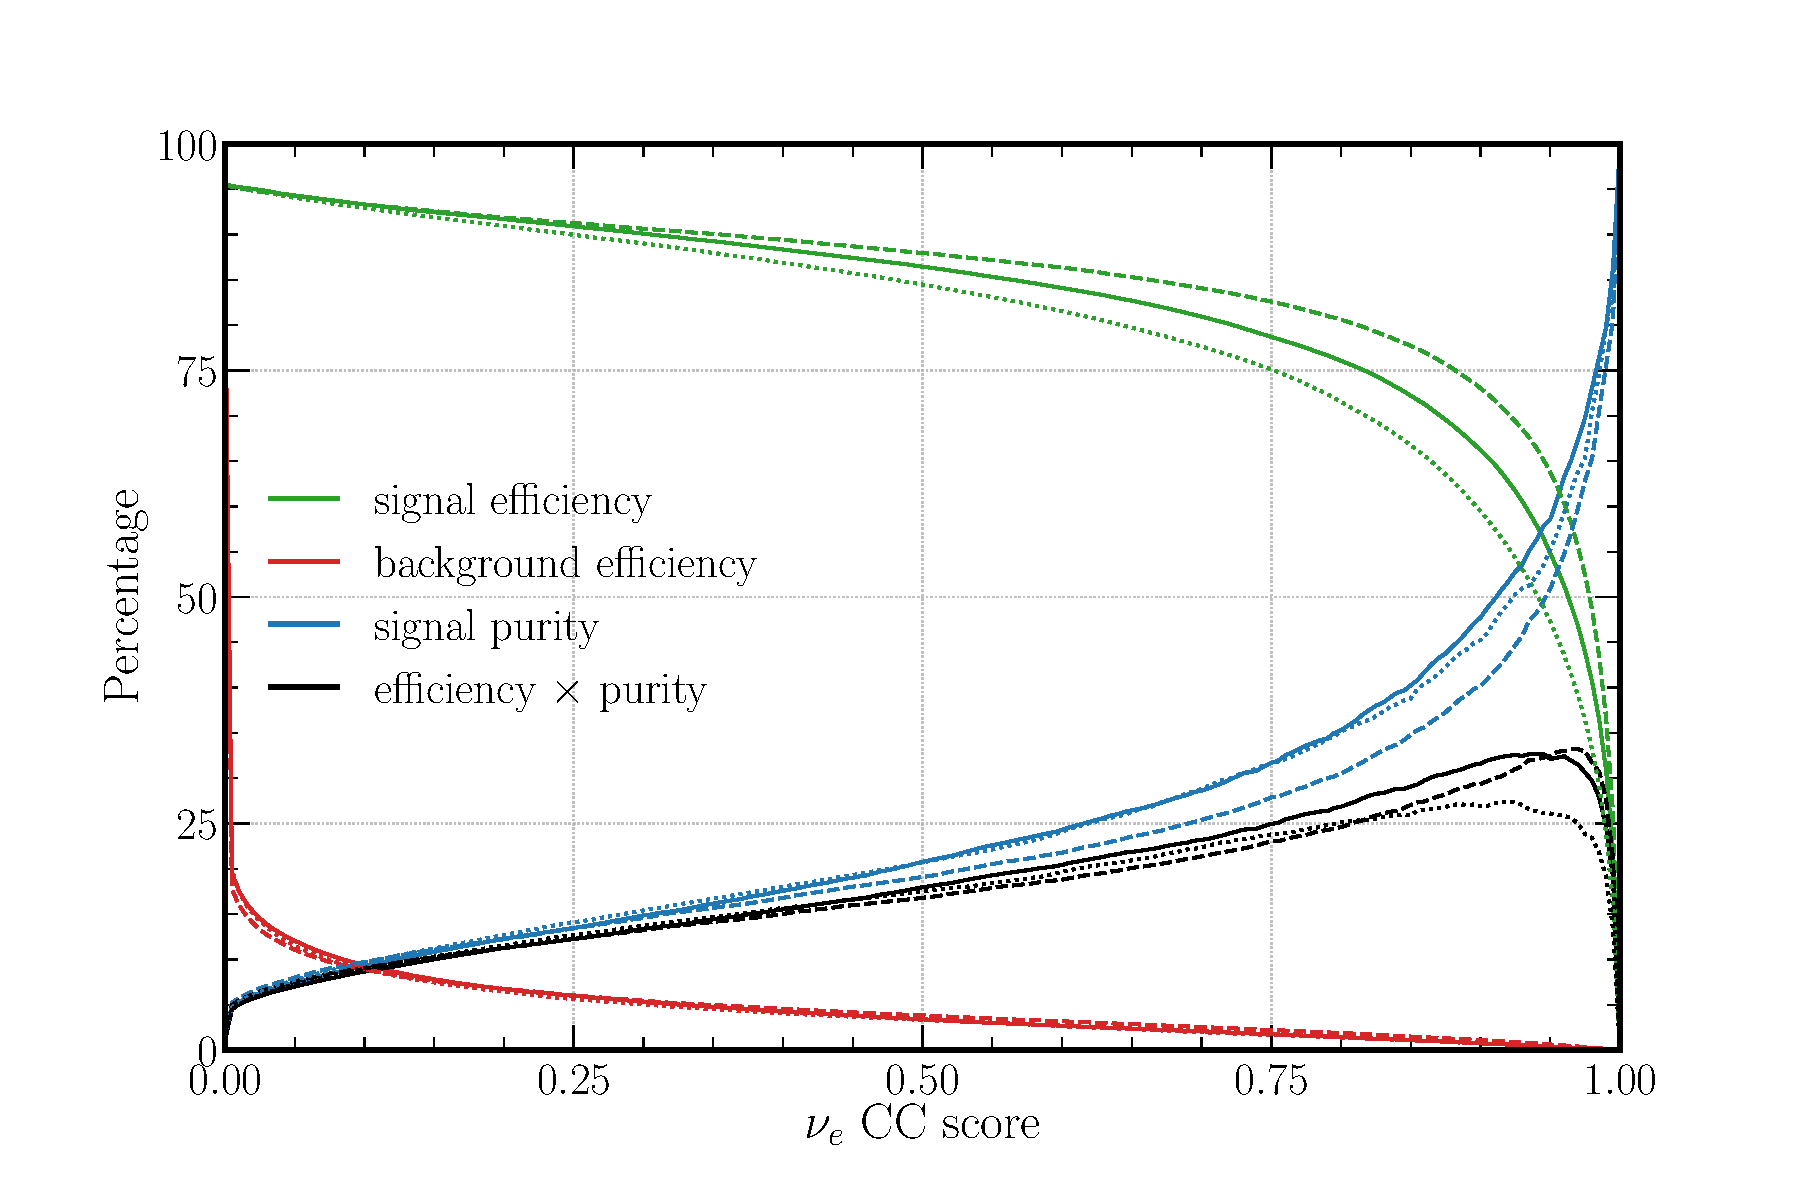
\includegraphics[width=0.6\textwidth]{diagrams/7-cvn/chipsnet/sample_nuel_eff_curves.pdf}
    \caption[sample nuel eff curves short]
    {both=solid, flux=dashed, uniform=dotted}
    \label{fig:sample_nuel_eff_curves}
\end{figure}

\begin{figure} % SAMPLE NUEL COMP CURVES DIAGRAM %
    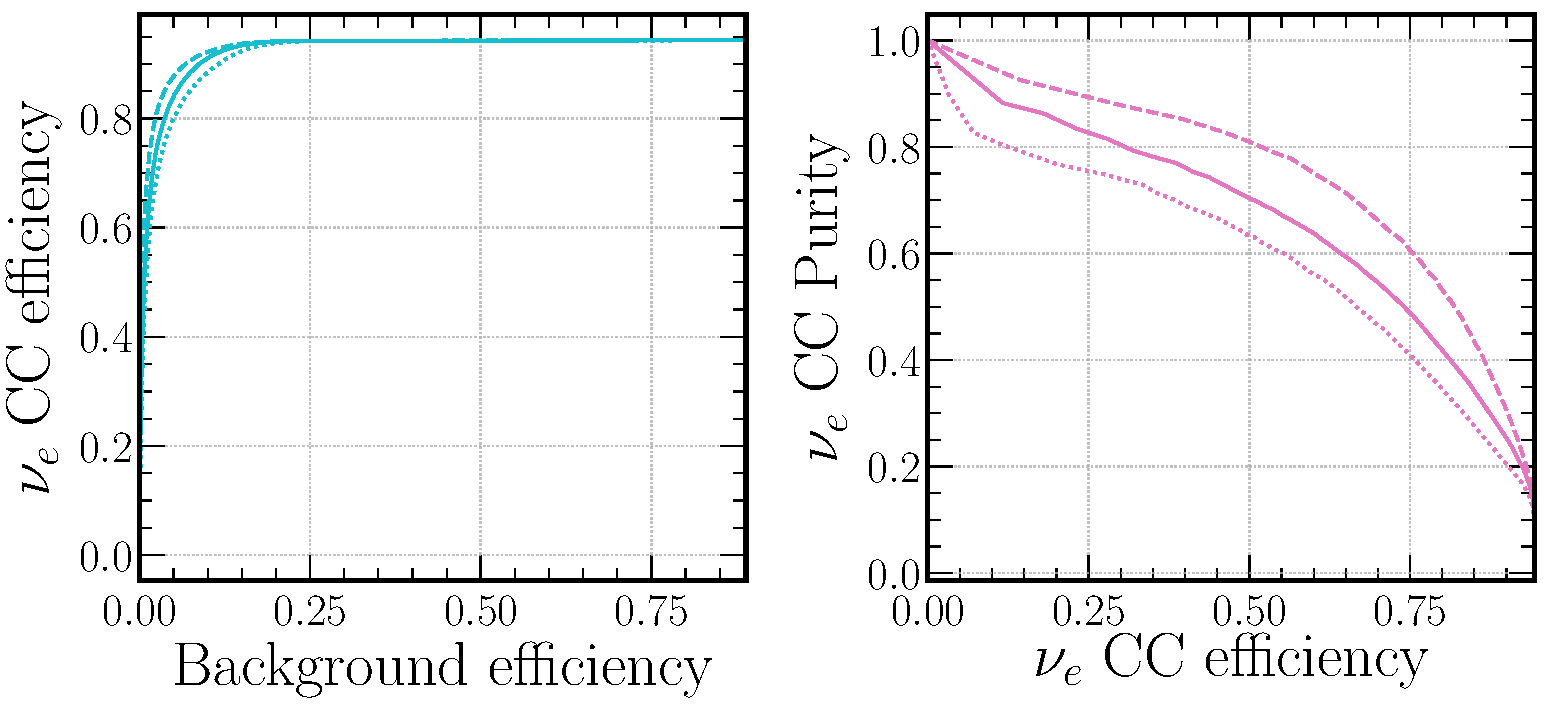
\includegraphics[width=0.8\textwidth]{diagrams/7-cvn/chipsnet/sample_nuel_comp_curves.pdf}
    \caption[sample nuel comp curves short]
    {both=solid, flux=dashed, uniform=dotted}
    \label{fig:sample_nuel_comp_curves}
\end{figure}

- Nuel-> ROC-AUC: 0.82559, PRC-AUC: 0.71155, S-Eff: 0.87661, S-Pur: 0.36928
- FOM1-> 0.46510, 0.93000, 53.44422, 8.34671, 15.75487, 0.67485, 0.68920
- FOM2-> 13.44645, 0.98500, 31.21664, 1.57028, 3.81933, 0.39418, 0.85277

- Nuel-> ROC-AUC: 0.81488, PRC-AUC: 0.56769, S-Eff: 0.79933, S-Pur: 0.34677
- FOM1-> 0.33905, 0.82500, 49.50120, 26.12079, 15.63656, 0.62506, 0.54243
- FOM2-> 8.44226, 0.92500, 36.01710, 11.59853, 6.60268, 0.45479, 0.66430

- Nuel-> ROC-AUC: 0.82063, PRC-AUC: 0.63426, S-Eff: 0.83421, S-Pur: 0.36814
- FOM1-> 0.38628, 0.84000, 52.60971, 19.59654, 18.26900, 0.66431, 0.58148
- FOM2-> 10.10769, 0.96000, 30.52599, 4.49055, 4.63030, 0.38545, 0.76995

\subsection{Which event representation to use} %%%%%%%%%%%%%%%%%%%%%%%%%%%%%%%%%%%%%%%%%%%%%%%%%%%
\label{sec:cvn_baseline_repr} %%%%%%%%%%%%%%%%%%%%%%%%%%%%%%%%%%%%%%%%%%%%%%%%%%%%%%%%%%%%%%%%%%%%

- Cern summer report in Ref.~\cite{theodore2016}
- New ideas with x+ x- mapping in Ref.~\cite{berns2020}
- Fraction of deposited charge in endcaps = 0.4769380479133997

\begin{figure} % NUEL EVENT DIAGRAM %
    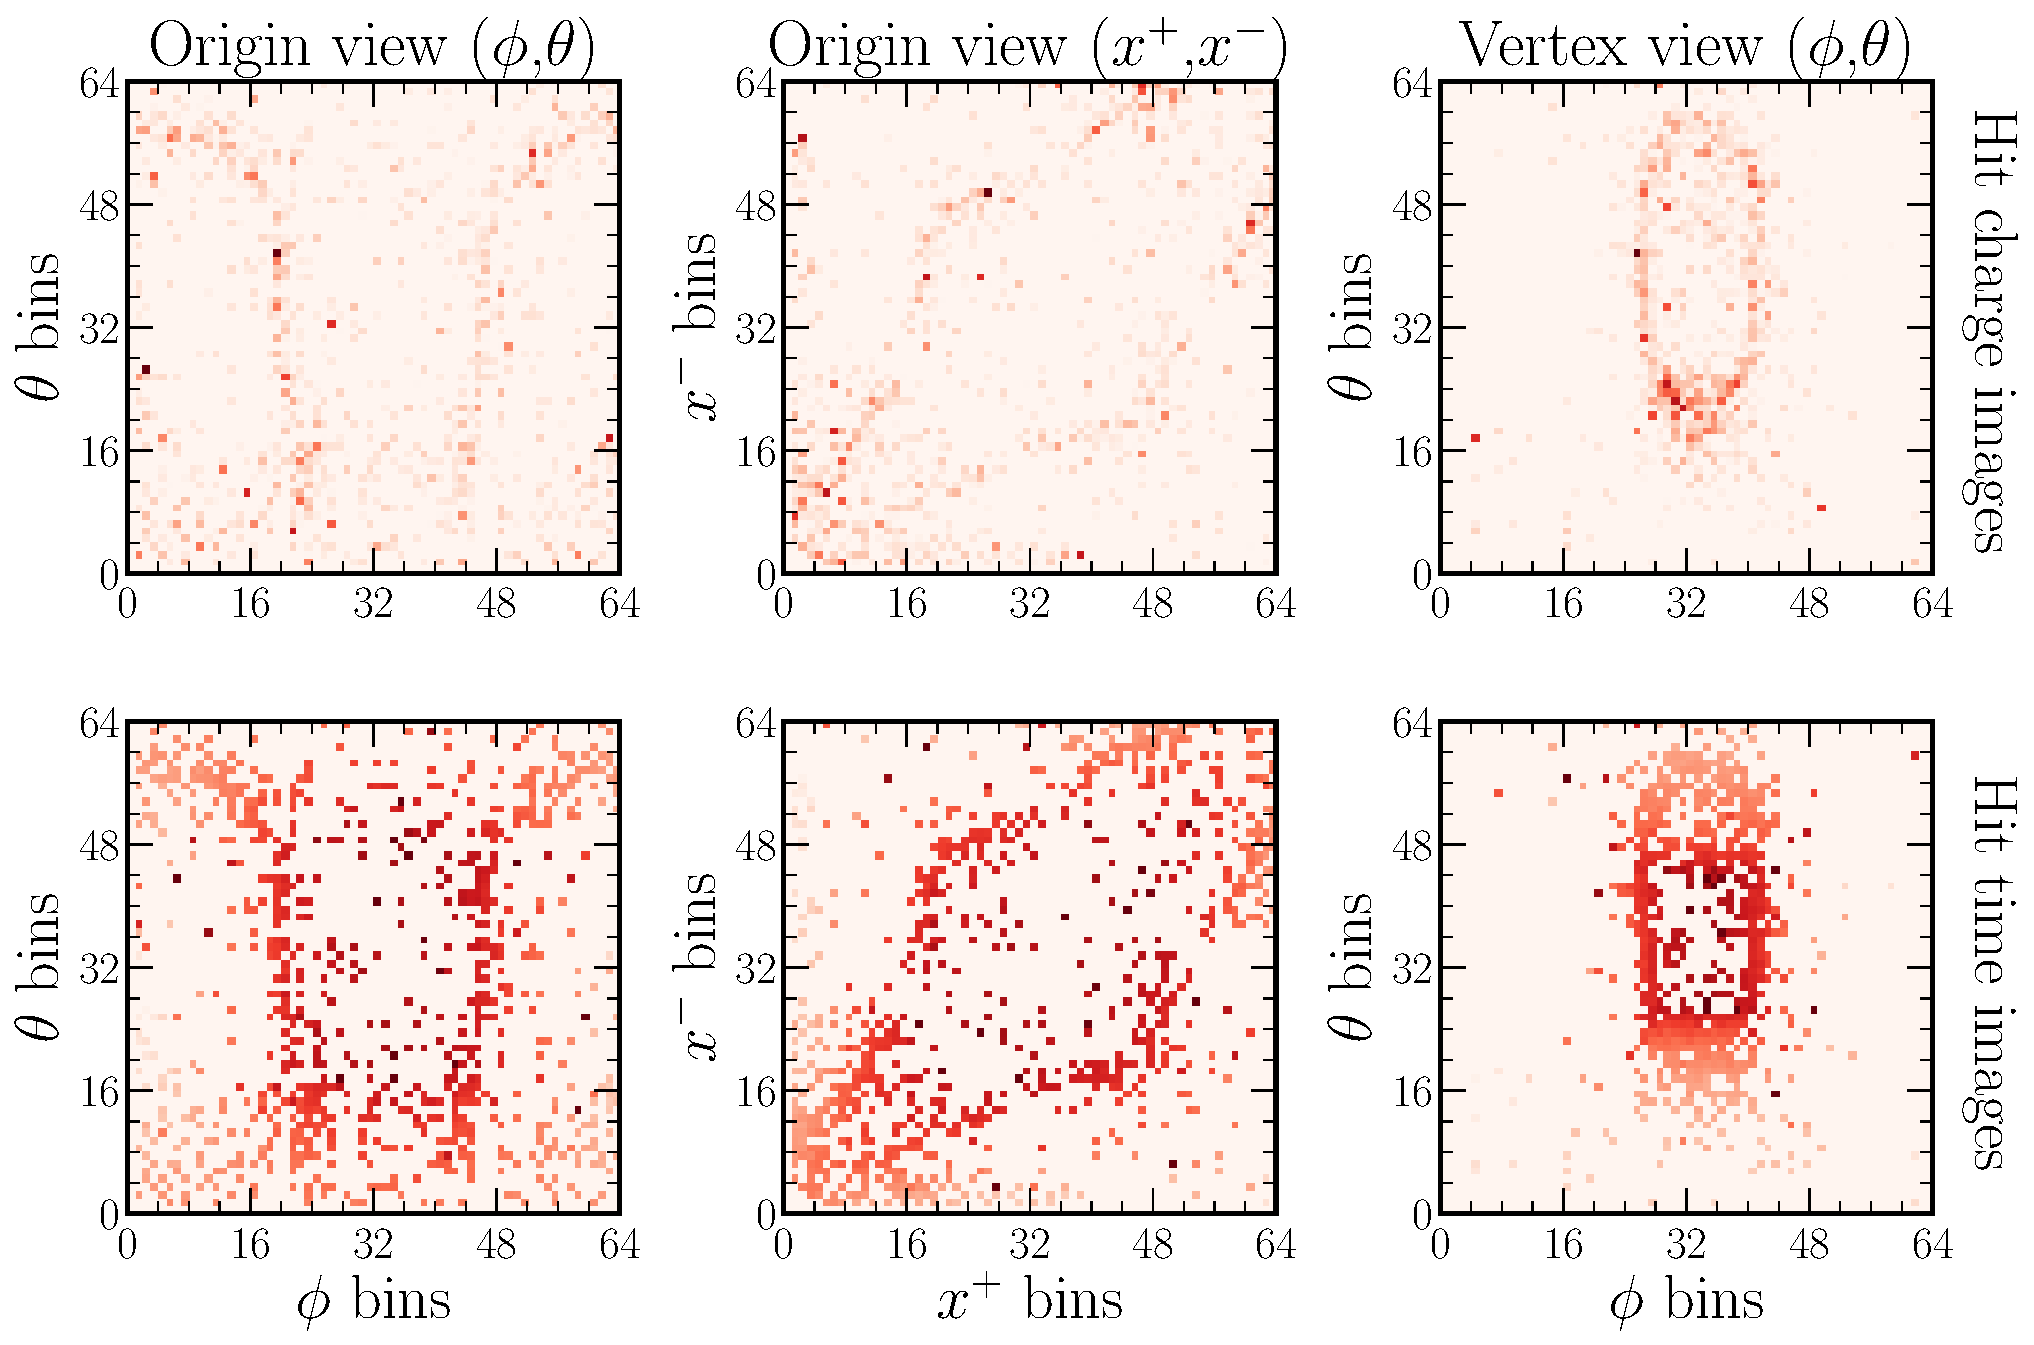
\includegraphics[width=0.8\textwidth]{diagrams/7-cvn/chipsnet/explore_nuel_ccres_event.pdf}
    \caption[explore nuel ccres event short]
    {3
        3307.41
        2777.48
            [  11 2212 2212  111 -999 -999 -999 -999 -999 -999 -999 -999 -999 -999
                -999 -999 -999 -999 -999 -999]
            [2777.48  1085.32   991.703  318.527 -999.    -999.    -999.    -999.
                -999.    -999.    -999.    -999.    -999.    -999.    -999.    -999.
                -999.    -999.    -999.    -999.   ]
        0}
    \label{fig:explore_nuel_ccres_event}
\end{figure}

\begin{figure} % NUMU EVENT DIAGRAM %
    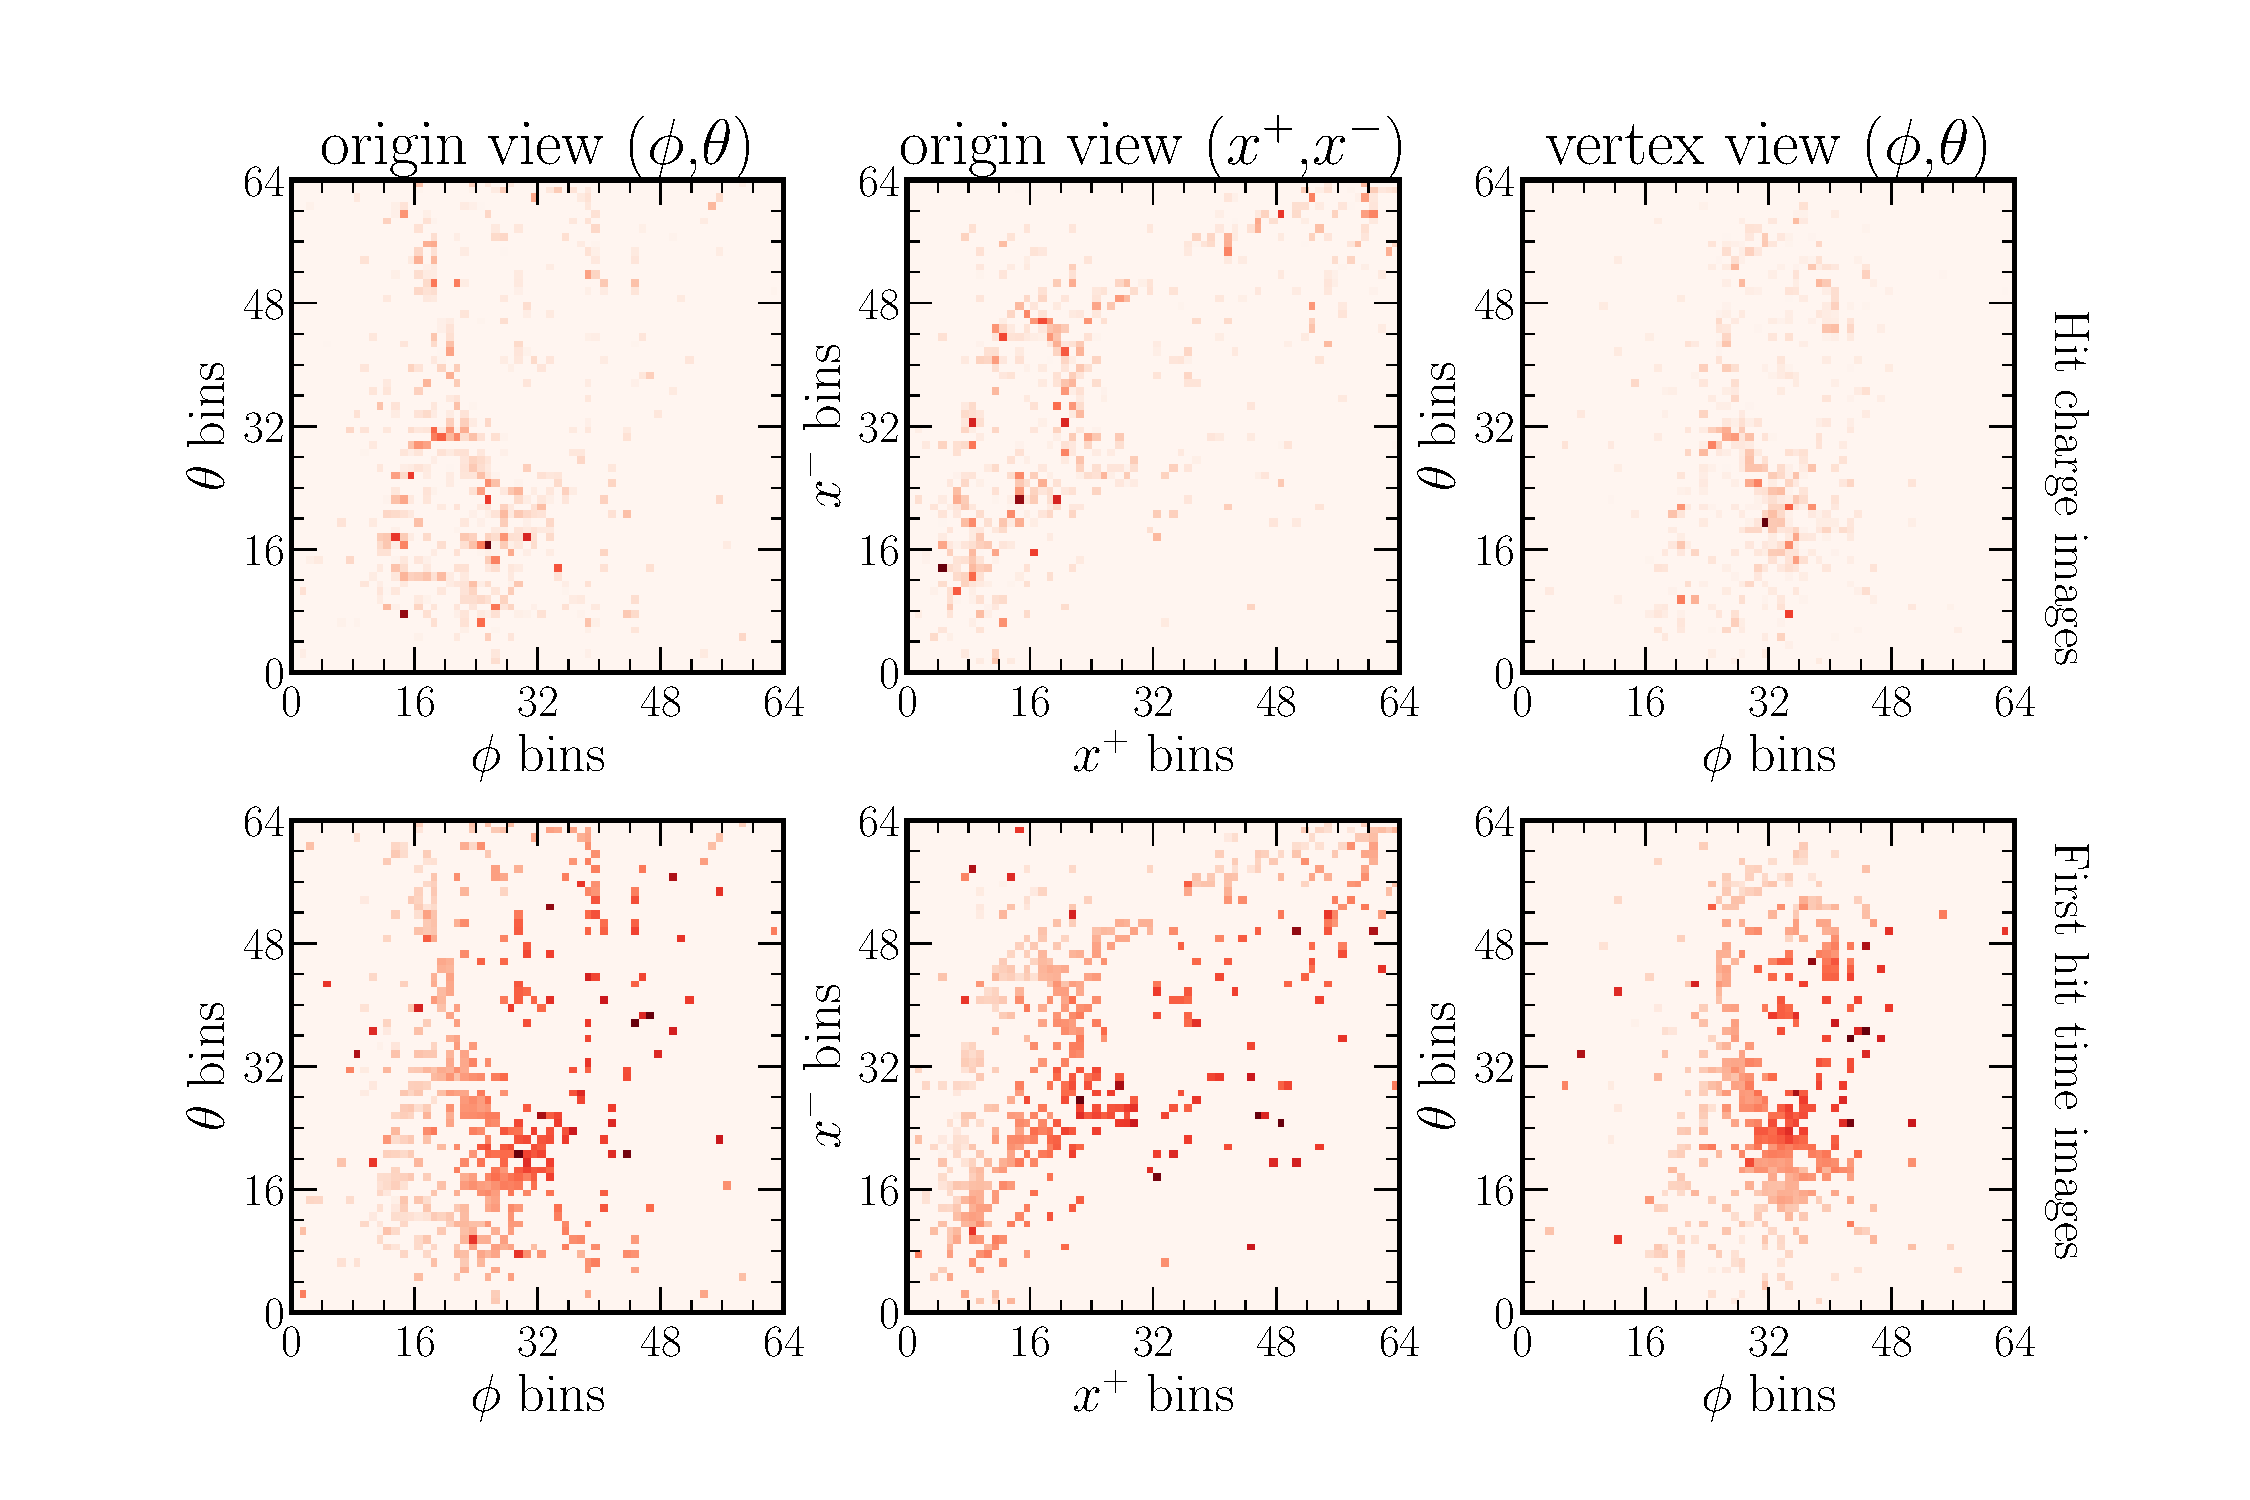
\includegraphics[width=0.8\textwidth]{diagrams/7-cvn/chipsnet/explore_numu_ccdis_event.pdf}
    \caption[explore numu ccdis event short]
    {91
        3520.17
        1862.55
            [2212   13 2112  211  211   22 -999 -999 -999 -999 -999 -999 -999 -999
                -999 -999 -999 -999 -999 -999]
            [2022.37  1862.55  1038.34   226.973  223.71     6.32  -999.    -999.
                -999.    -999.    -999.    -999.    -999.    -999.    -999.    -999.
                -999.    -999.    -999.    -999.   ]
        0}
    \label{fig:explore_numu_ccdis_event}
\end{figure}

\begin{figure} % NC EVENT DIAGRAM %
    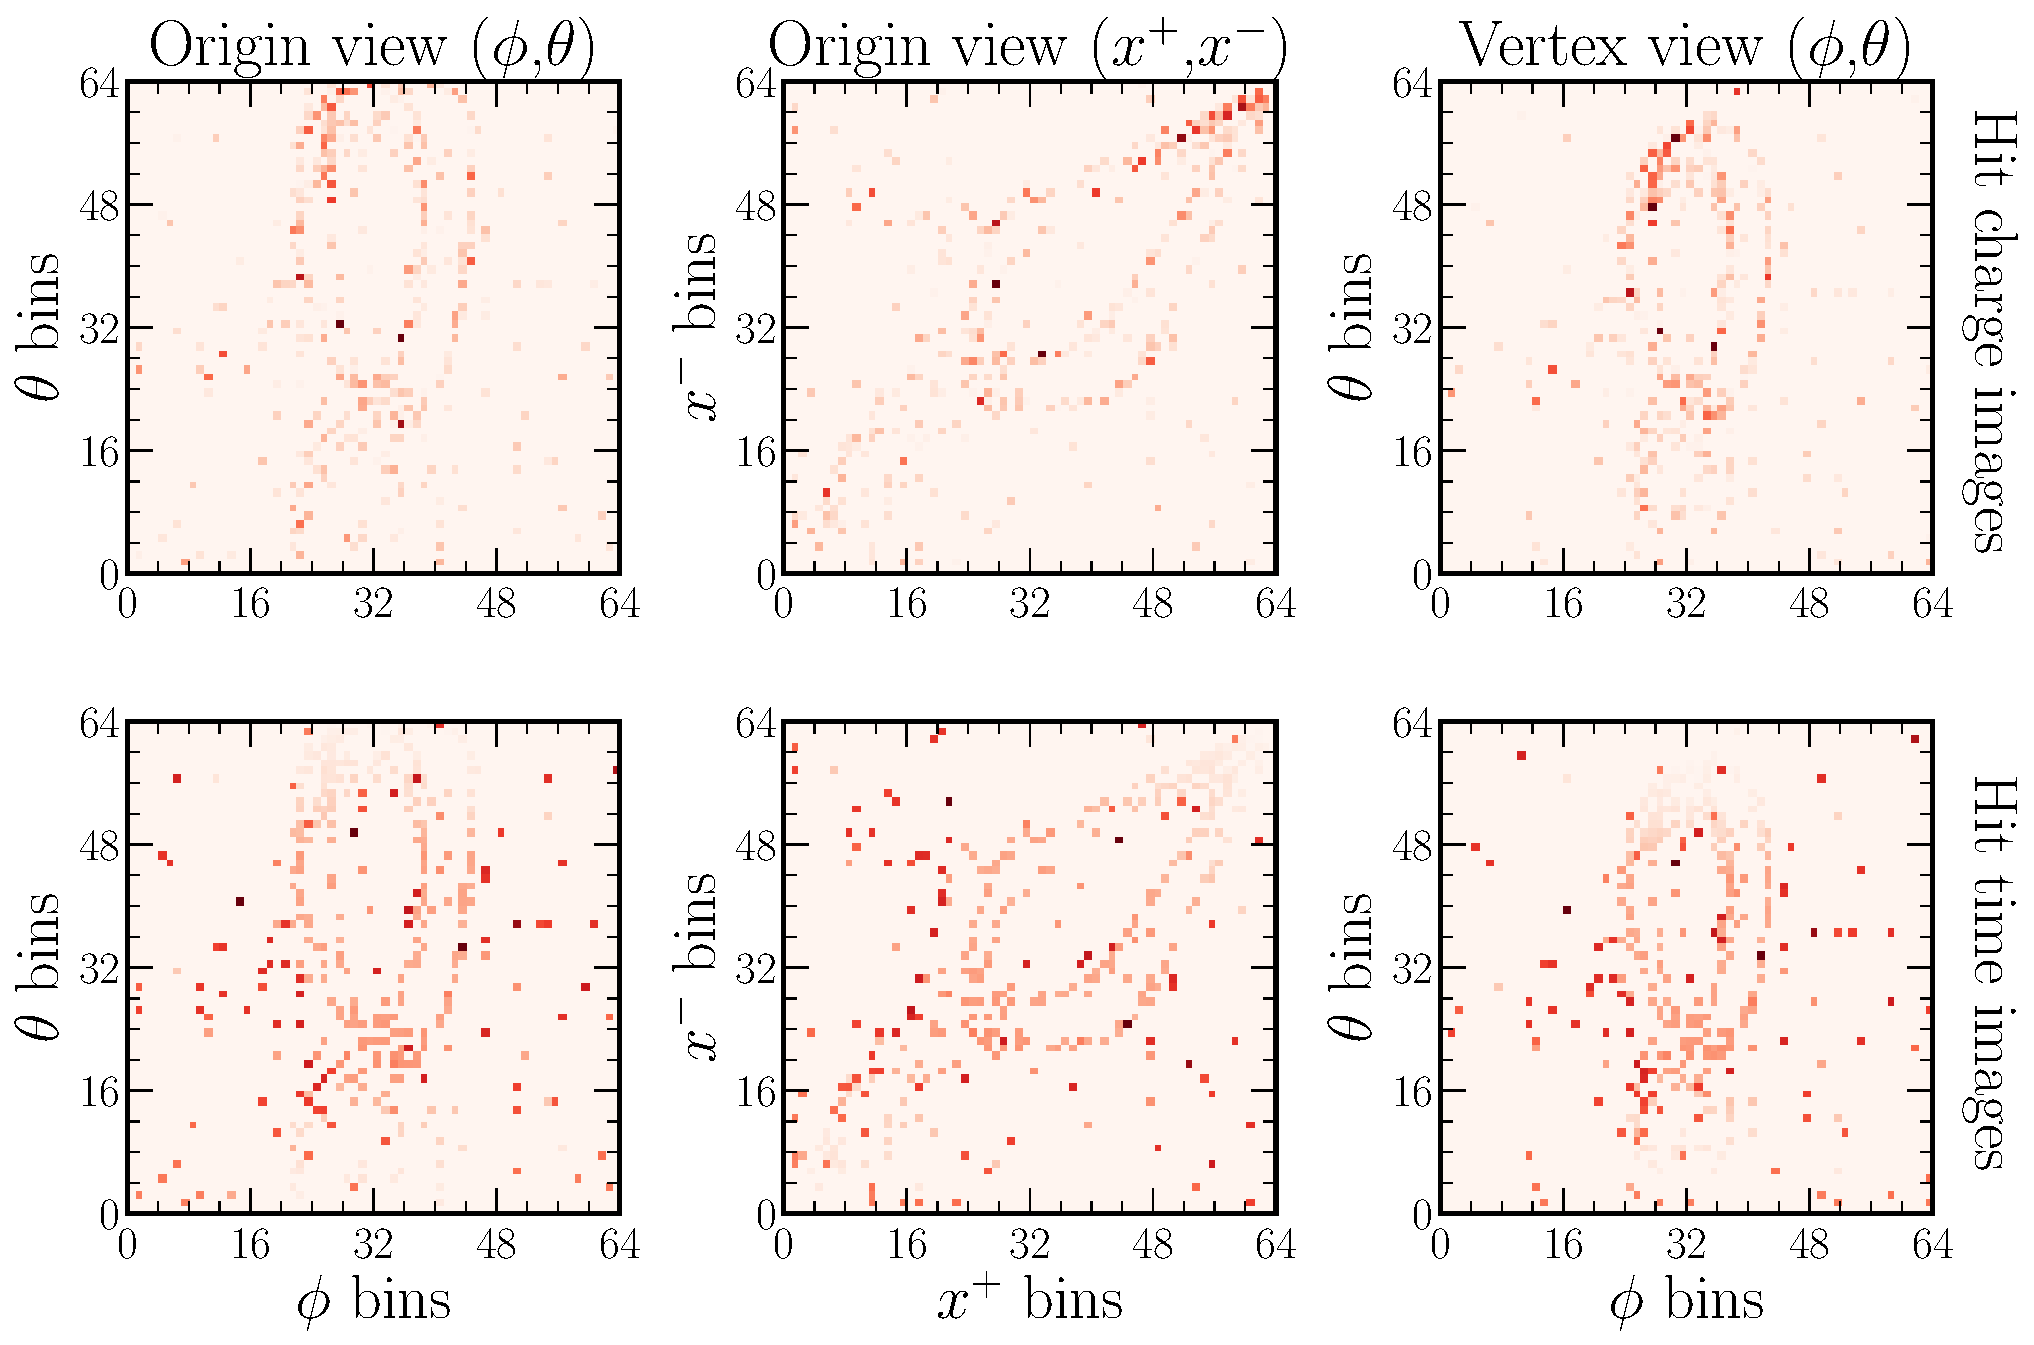
\includegraphics[width=0.8\textwidth]{diagrams/7-cvn/chipsnet/explore_nuel_ncdis_event.pdf}
    \caption[explore nuel ncdis event short]
    {92
    9301.59
    -1.0
    [  12 2212  211 2212 2212 2112 -999 -999 -999 -999 -999 -999 -999 -999
    -999 -999 -999 -999 -999 -999]
    [4731.25  2635.15  2511.54  1046.97   998.676  993.868 -999.    -999.
    -999.    -999.    -999.    -999.    -999.    -999.    -999.    -999.
    -999.    -999.    -999.    -999.   ]
    -1
    }
    \label{fig:explore_nuel_ncdis_event}
\end{figure}

\begin{figure} % COSMIC MUON EVENT DIAGRAM %
    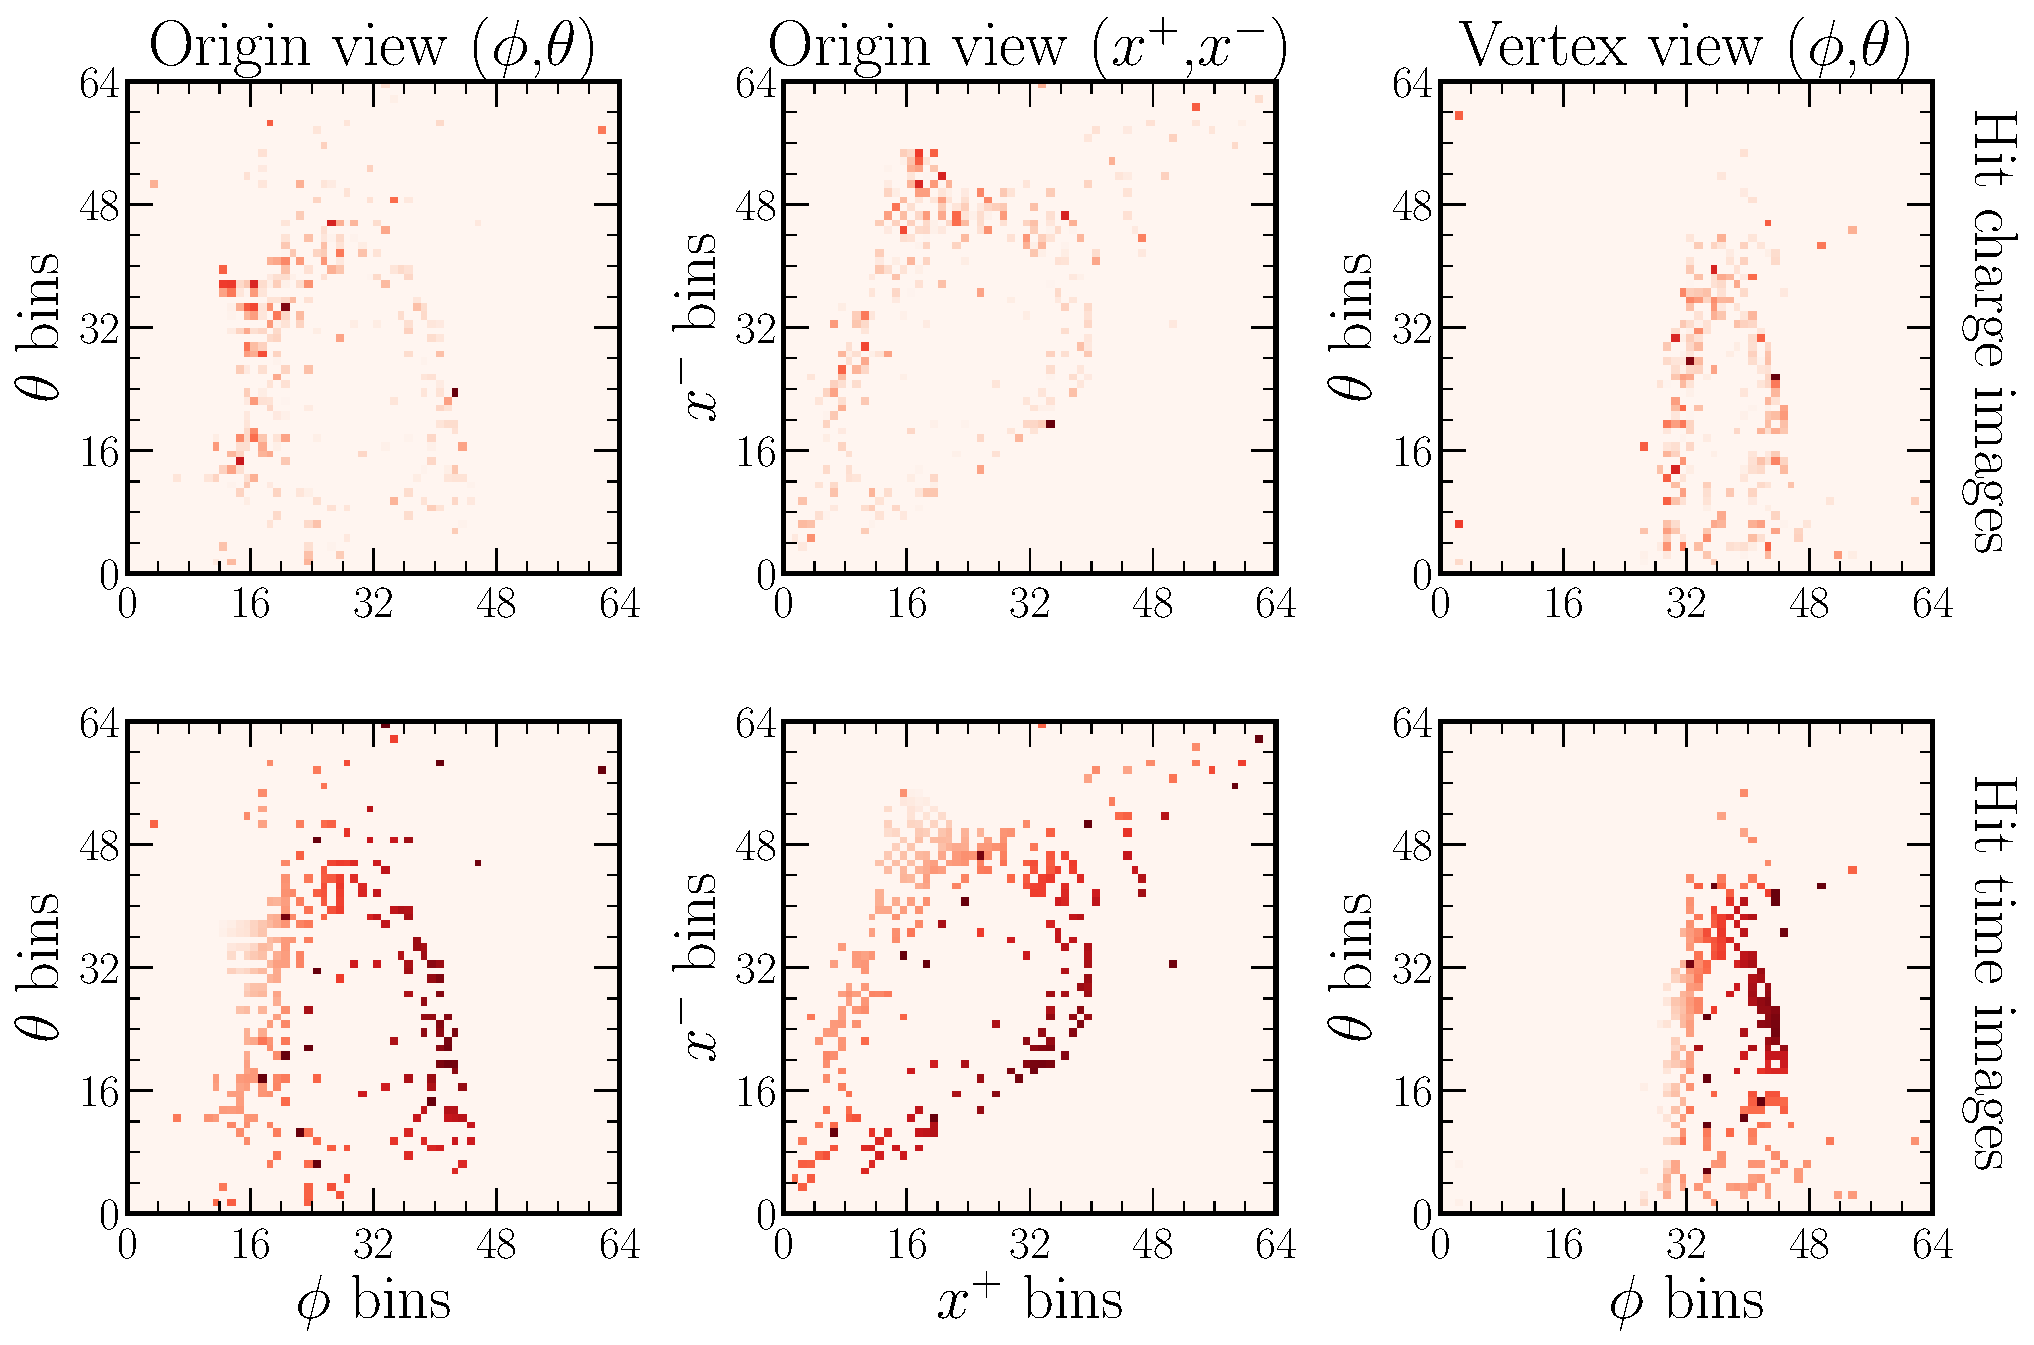
\includegraphics[width=0.8\textwidth]{diagrams/7-cvn/chipsnet/explore_cosmic_event.pdf}
    \caption[explore cosmic event short]
    {100
        2928.5
        2928.5
            [  13 -999 -999 -999 -999 -999 -999 -999 -999 -999 -999 -999 -999 -999
                -999 -999 -999 -999 -999 -999]
            [2928.5 -999.  -999.  -999.  -999.  -999.  -999.  -999.  -999.  -999.
                -999.  -999.  -999.  -999.  -999.  -999.  -999.  -999.  -999.  -999. ]
        0}
    \label{fig:explore_cosmic_event}
\end{figure}

\begin{figure} % HOUGH REPRESENTATIONS DIAGRAM %
    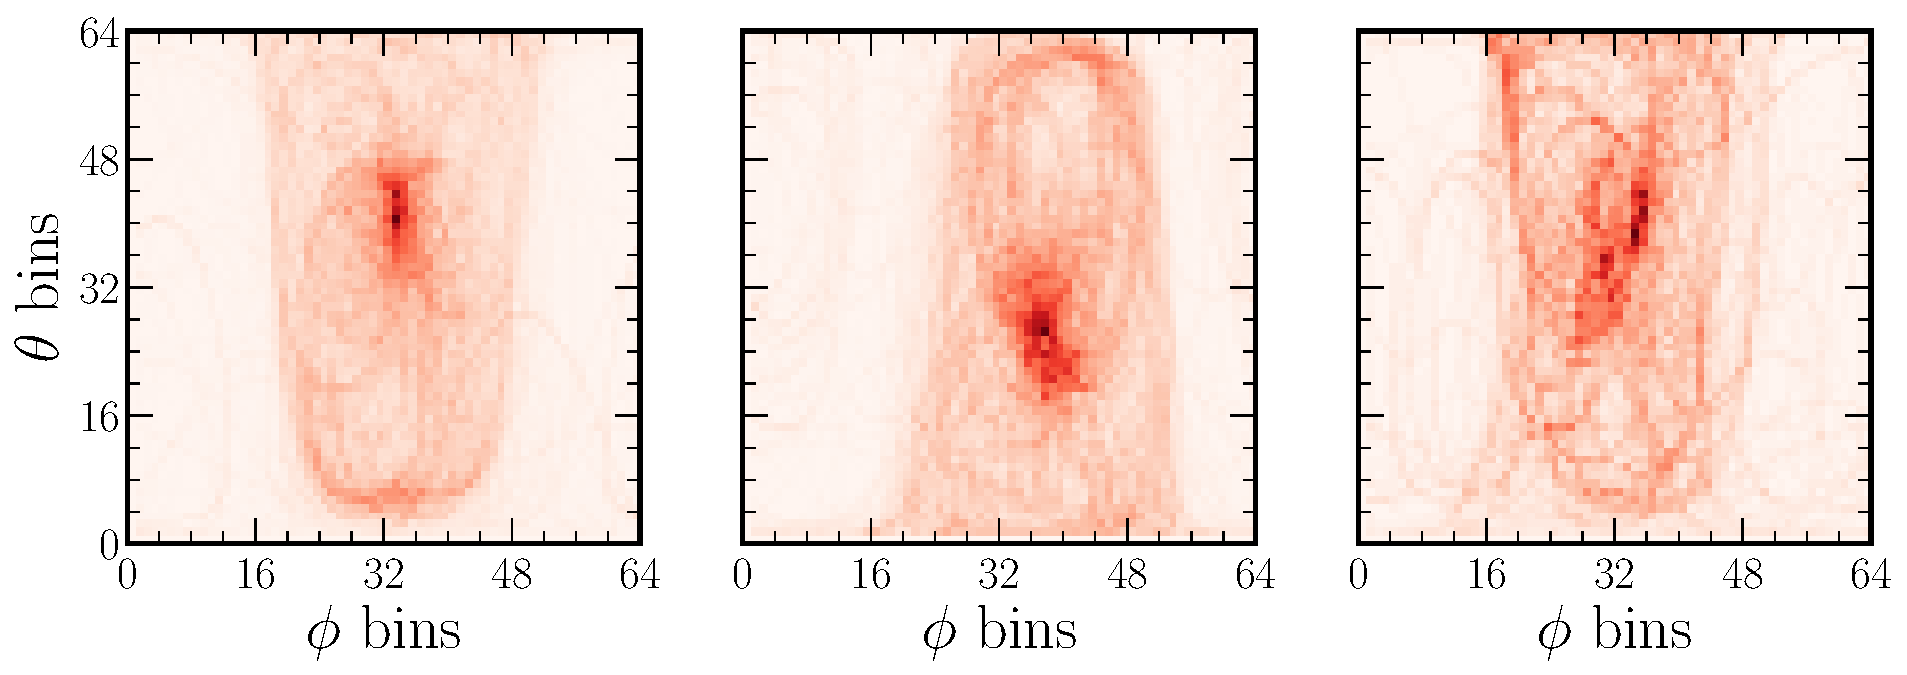
\includegraphics[width=\textwidth]{diagrams/7-cvn/chipsnet/explore_hough_events.pdf}
    \caption[example hough events short]
    {example hough events long}
    \label{fig:example_hough_events}
\end{figure}

\begin{figure} % VTX POSITIONS DIAGRAM %
    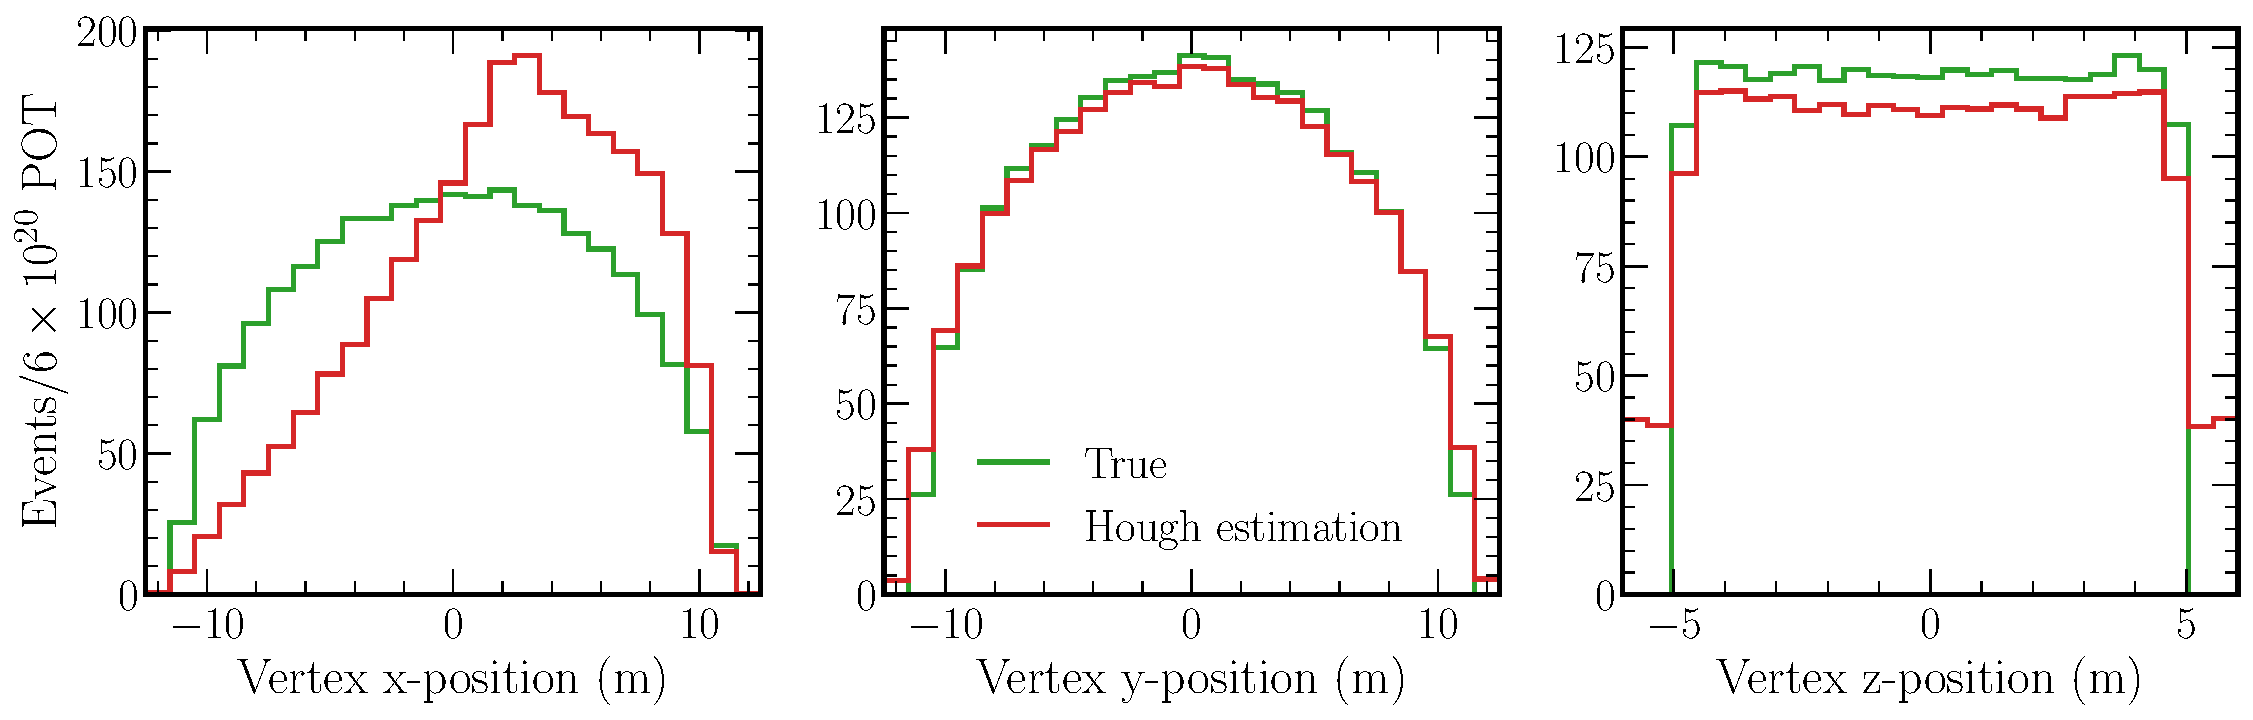
\includegraphics[width=\textwidth]{diagrams/7-cvn/chipsnet/explore_vtx_positions.pdf}
    \caption[explore vtx positions short]
    {explore vtx positions long}
    \label{fig:explore_vtx_positions}
\end{figure}

\begin{figure} % HOUGH VTX RES DIAGRAM %
    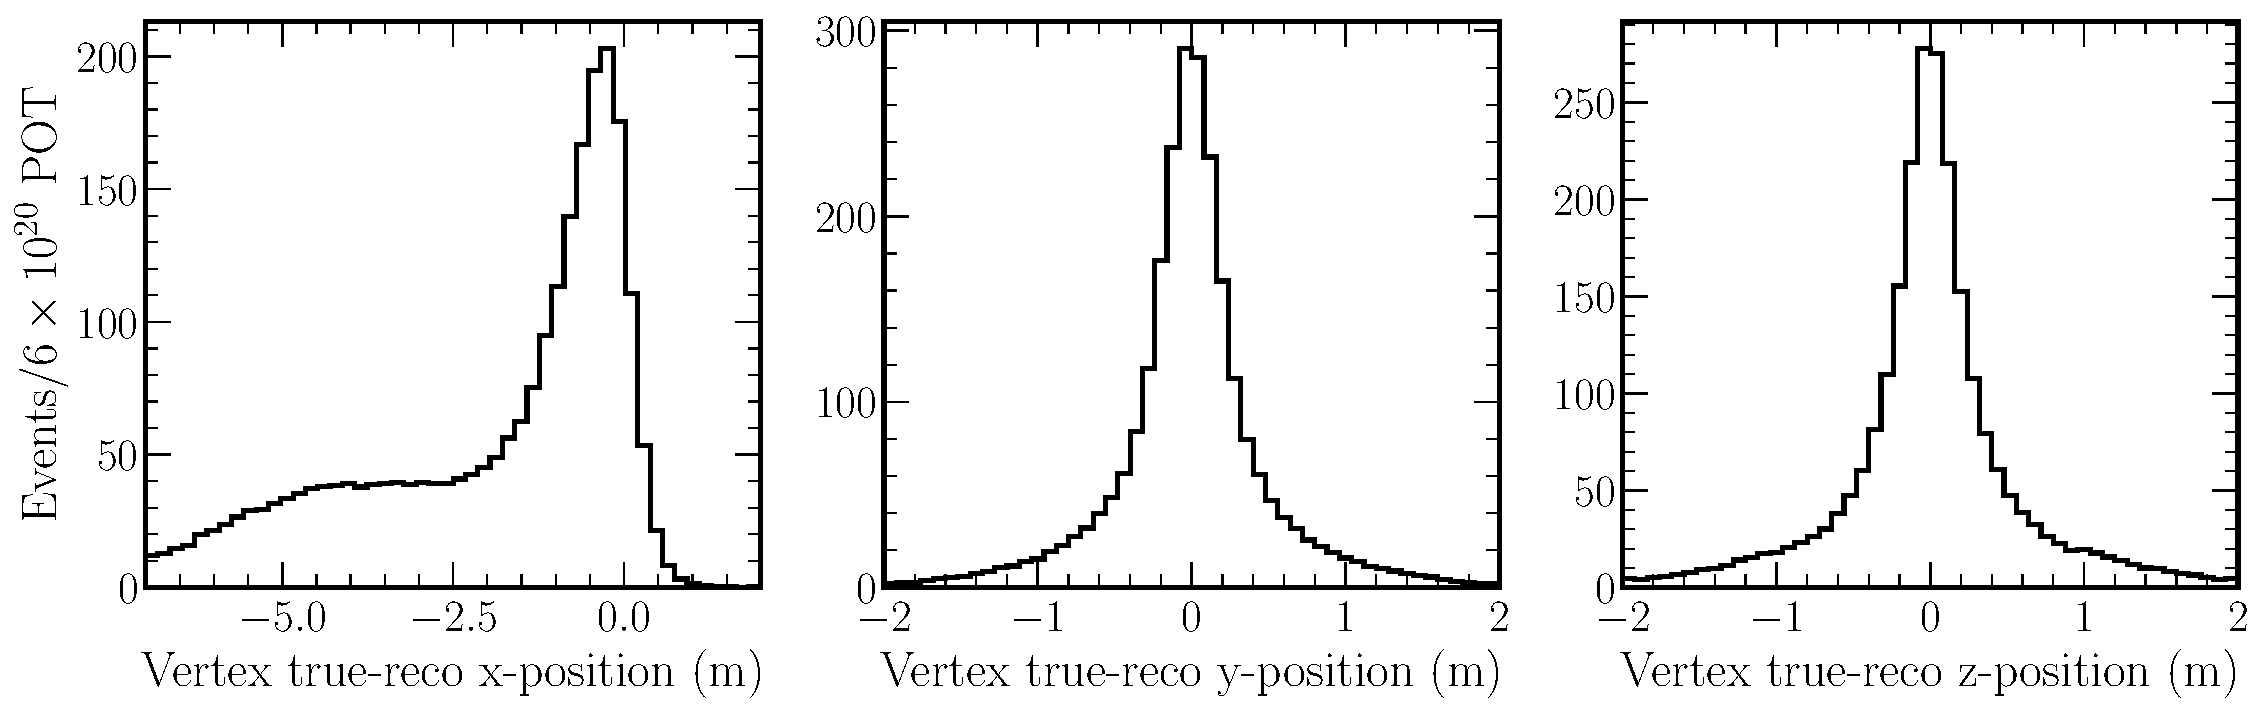
\includegraphics[width=\textwidth]{diagrams/7-cvn/chipsnet/explore_true_reco_vtx.pdf}
    \caption[explore true reco vtx short]
    {explore true reco vtx long}
    \label{fig:explore_true_reco_vtx}
\end{figure}

- Nuel-> ROC-AUC: 0.82509, PRC-AUC: 0.70686, S-Eff: 0.87786, S-Pur: 0.35433
- FOM1-> 0.46118, 0.93000, 52.98765, 8.61419, 15.27335, 0.66908, 0.68927
- FOM2-> 13.26595, 0.98500, 29.74203, 1.43964, 3.58684, 0.37556, 0.85543

- Nuel-> ROC-AUC: 0.82178, PRC-AUC: 0.67486, S-Eff: 0.87439, S-Pur: 0.29114
- FOM1-> 0.42202, 0.95500, 50.65626, 10.27209, 15.82963, 0.63948, 0.65995
- FOM2-> 12.53864, 0.99000, 29.40728, 1.75353, 3.74706, 0.37123, 0.84243

- Nuel-> ROC-AUC: 0.82116, PRC-AUC: 0.66987, S-Eff: 0.86660, S-Pur: 0.29764
- FOM1-> 0.41895, 0.94500, 50.97483, 10.86474, 16.45768, 0.64350, 0.65104
- FOM2-> 12.22739, 0.99000, 28.43808, 1.74364, 3.66555, 0.35900, 0.84019

\begin{figure} % REPR NUEL EFF CURVES DIAGRAM %
    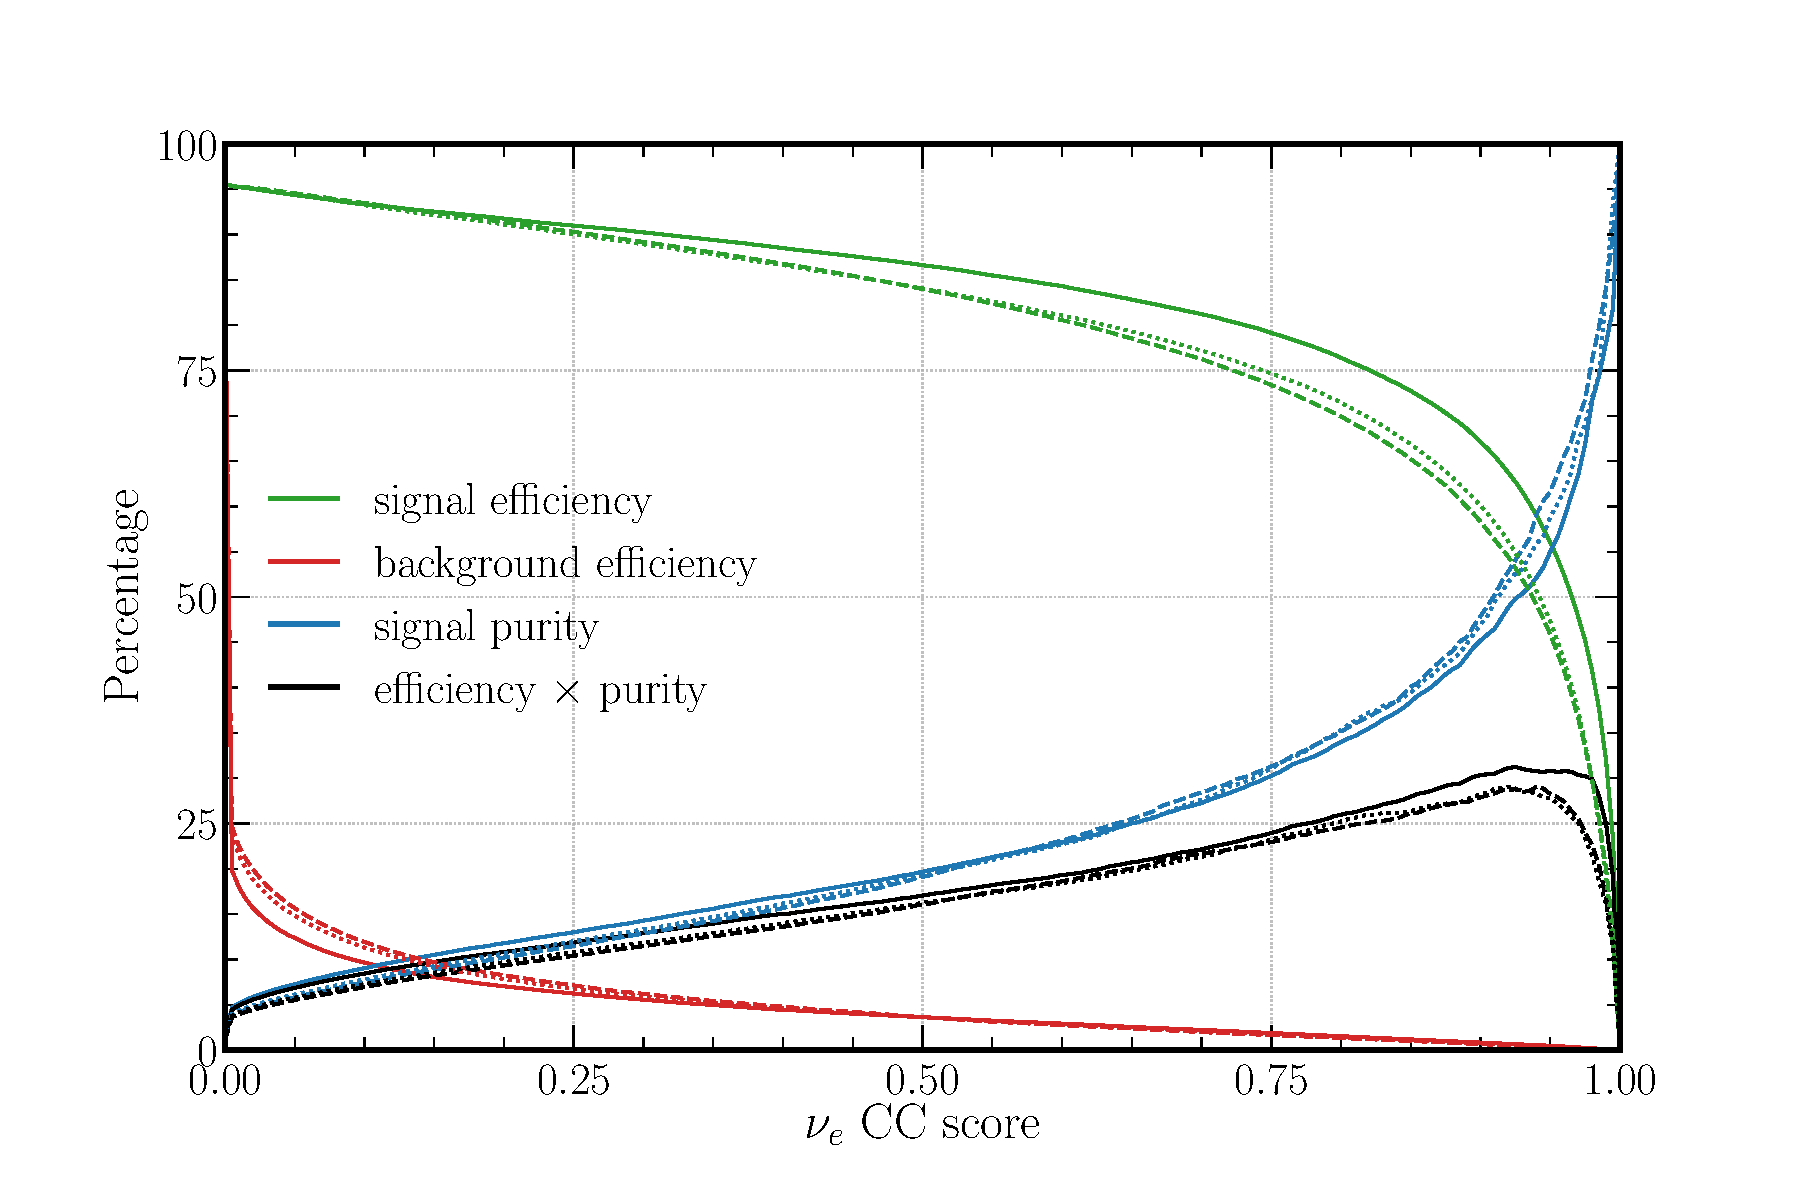
\includegraphics[width=0.6\textwidth]{diagrams/7-cvn/chipsnet/repr_nuel_eff_curves.pdf}
    \caption[repr nuel eff curves short]
    {v=solid, o=dashed, i=dotted}
    \label{fig:repr_nuel_eff_curves}
\end{figure}

\begin{figure} % REPR NUEL COMP CURVES DIAGRAM %
    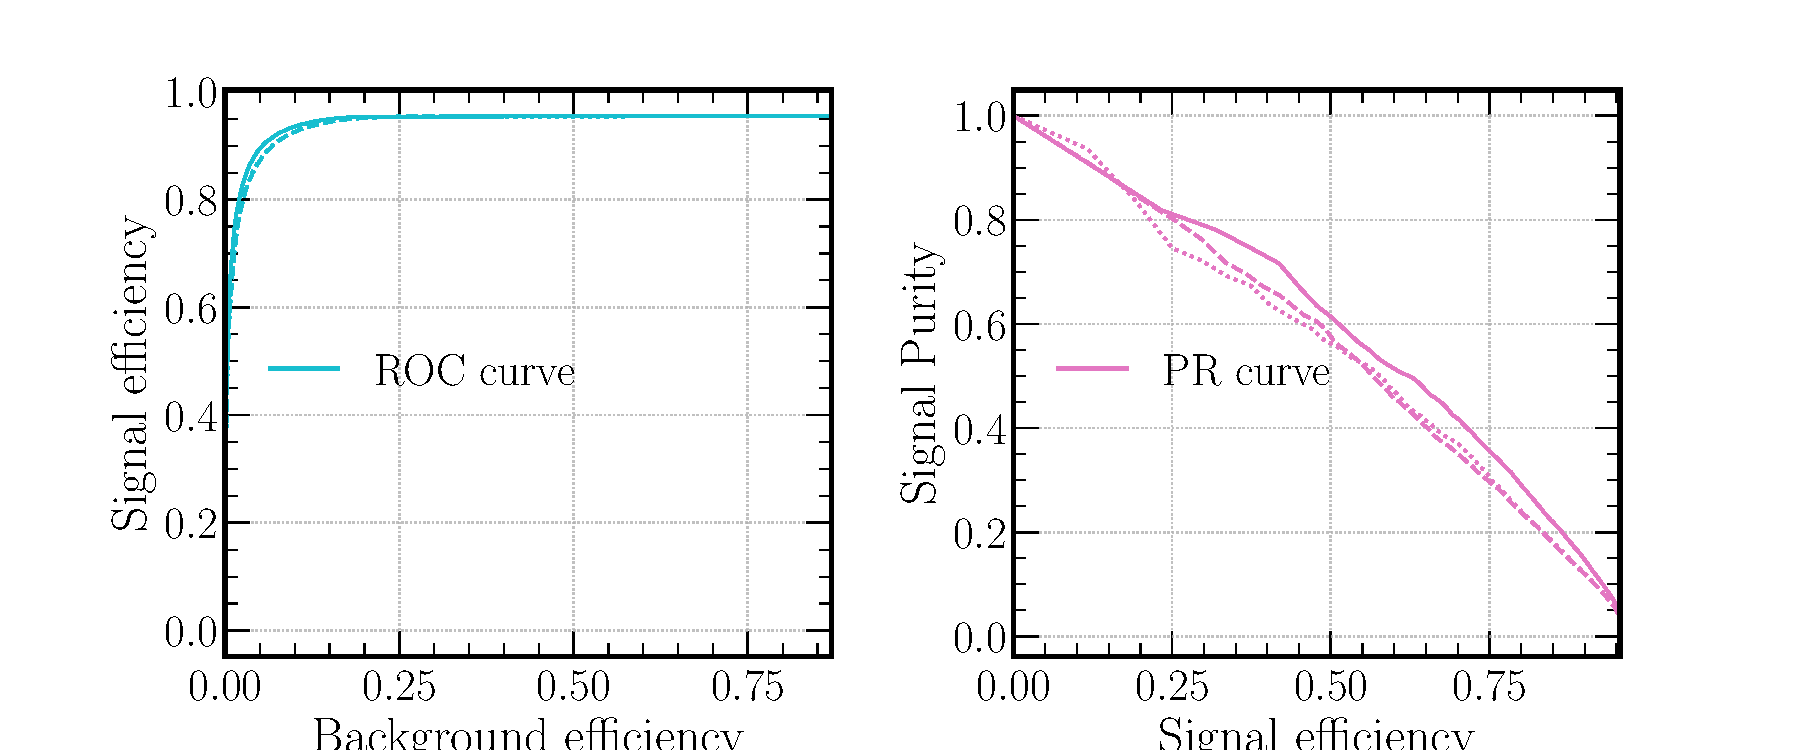
\includegraphics[width=0.8\textwidth]{diagrams/7-cvn/chipsnet/repr_nuel_comp_curves.pdf}
    \caption[repr nuel comp curves short]
    {v=solid, o=dashed, i=dotted}
    \label{fig:repr_nuel_comp_curves}
\end{figure}

\begin{figure} % REPR NUMU EFF CURVES DIAGRAM %
    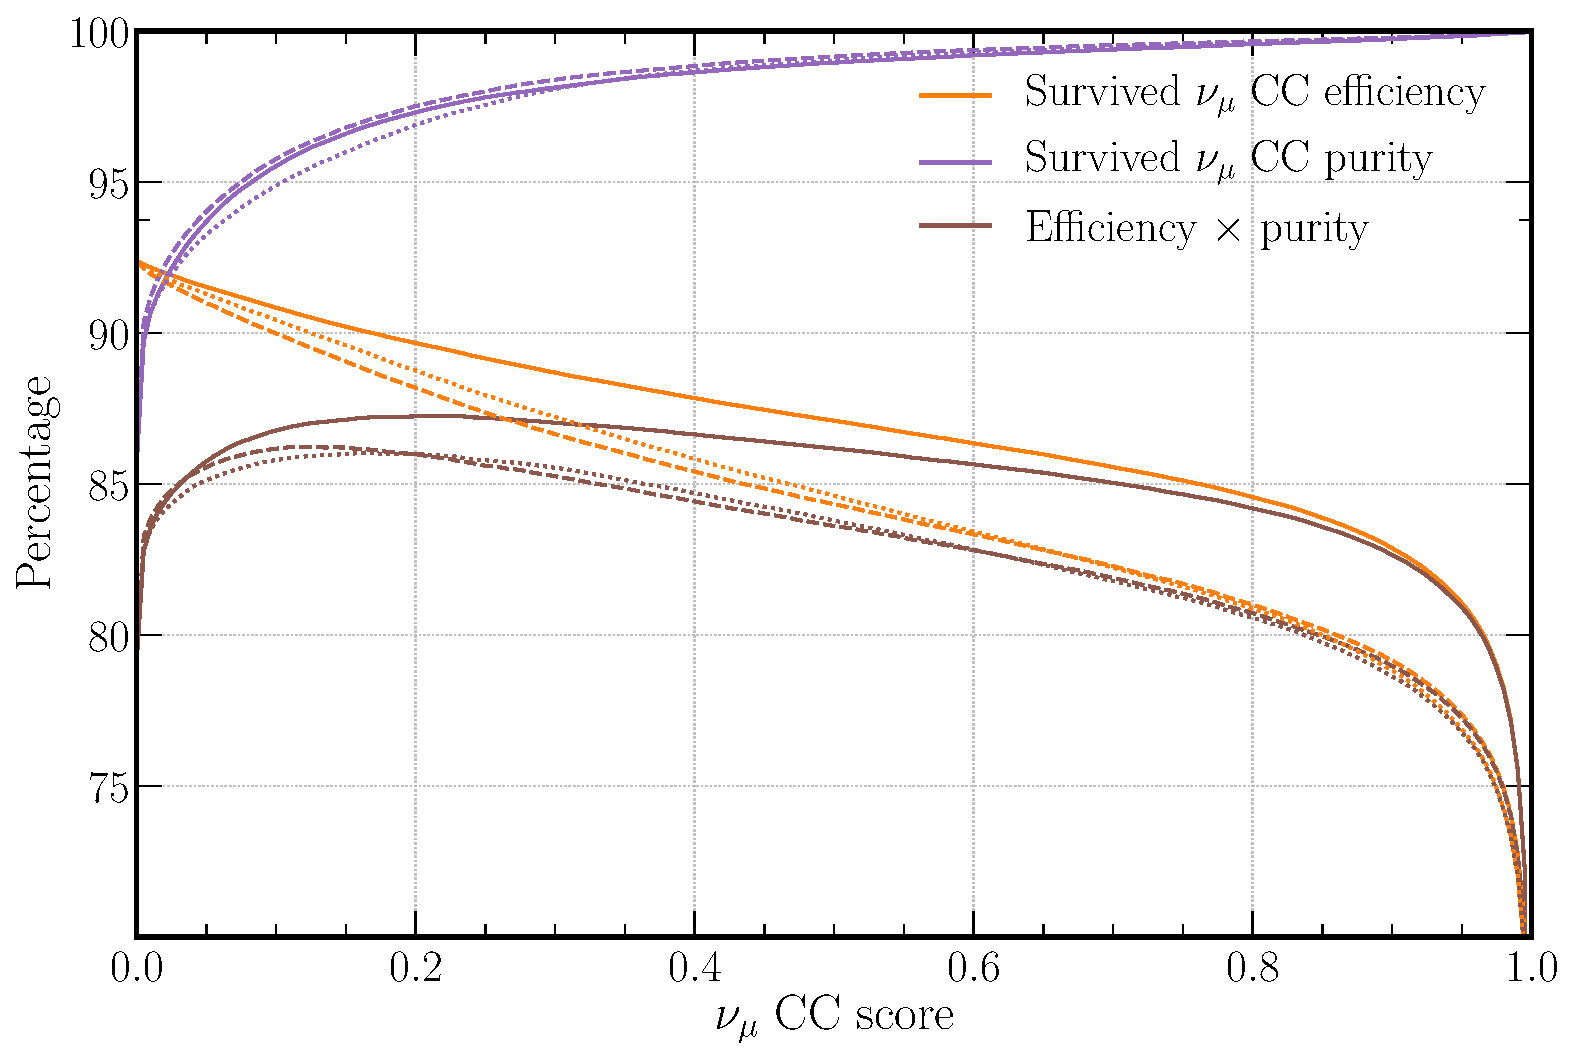
\includegraphics[width=0.6\textwidth]{diagrams/7-cvn/chipsnet/repr_numu_eff_curves.pdf}
    \caption[repr numu eff curves short]
    {v=solid, o=dashed, i=dotted}
    \label{fig:repr_numu_eff_curves}
\end{figure}

\begin{figure} % REPR NUMU COMP CURVES DIAGRAM %
    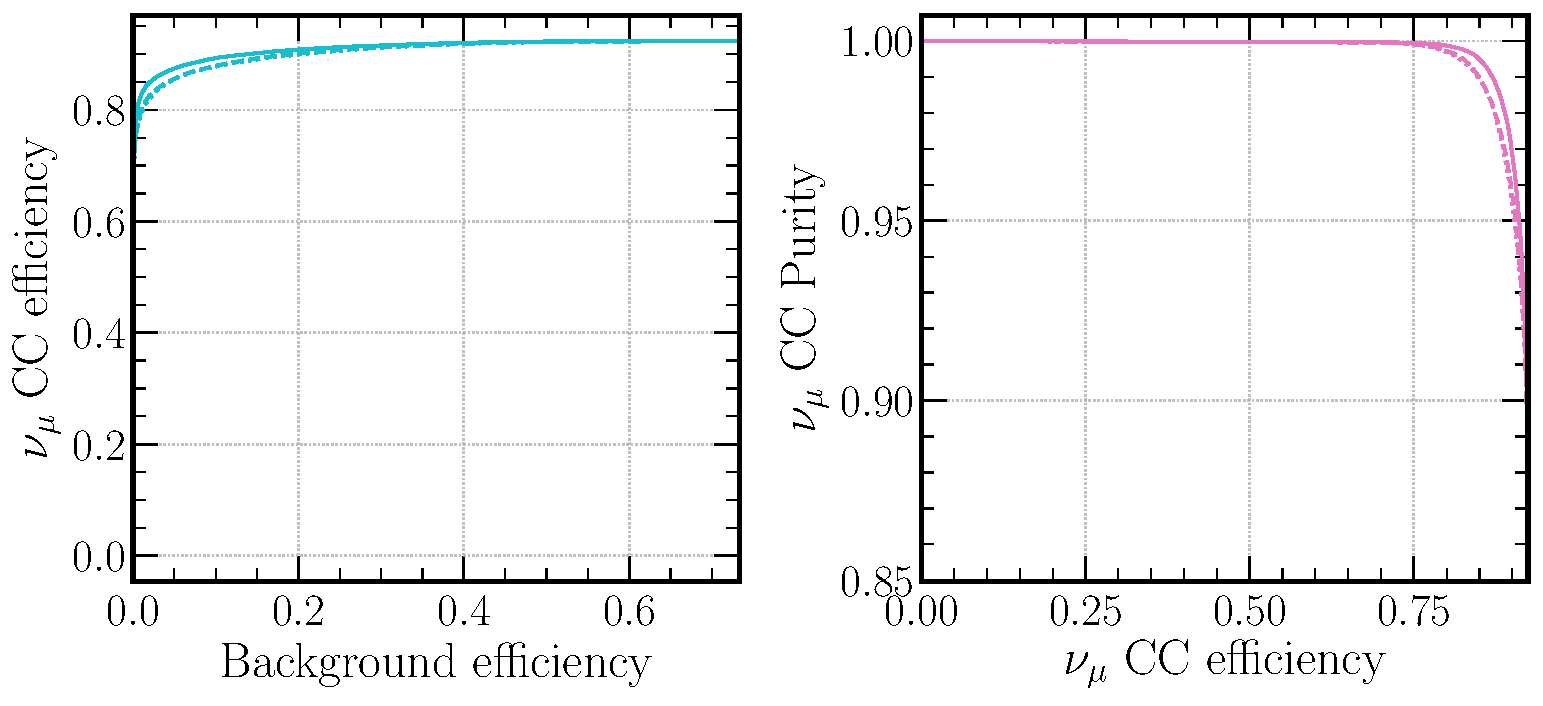
\includegraphics[width=0.8\textwidth]{diagrams/7-cvn/chipsnet/repr_numu_comp_curves.pdf}
    \caption[repr numu comp curves short]
    {v=solid, o=dashed, i=dotted}
    \label{fig:repr_numu_comp_curves}
\end{figure}

\subsection{Which channels to use} %%%%%%%%%%%%%%%%%%%%%%%%%%%%%%%%%%%%%%%%%%%%%%%%%%%%%%%%%%%%%%%
\label{sec:cvn_baseline_channel} %%%%%%%%%%%%%%%%%%%%%%%%%%%%%%%%%%%%%%%%%%%%%%%%%%%%%%%%%%%%%%%%%

\begin{figure} % CHANNEL NUEL EFF CURVES DIAGRAM %
    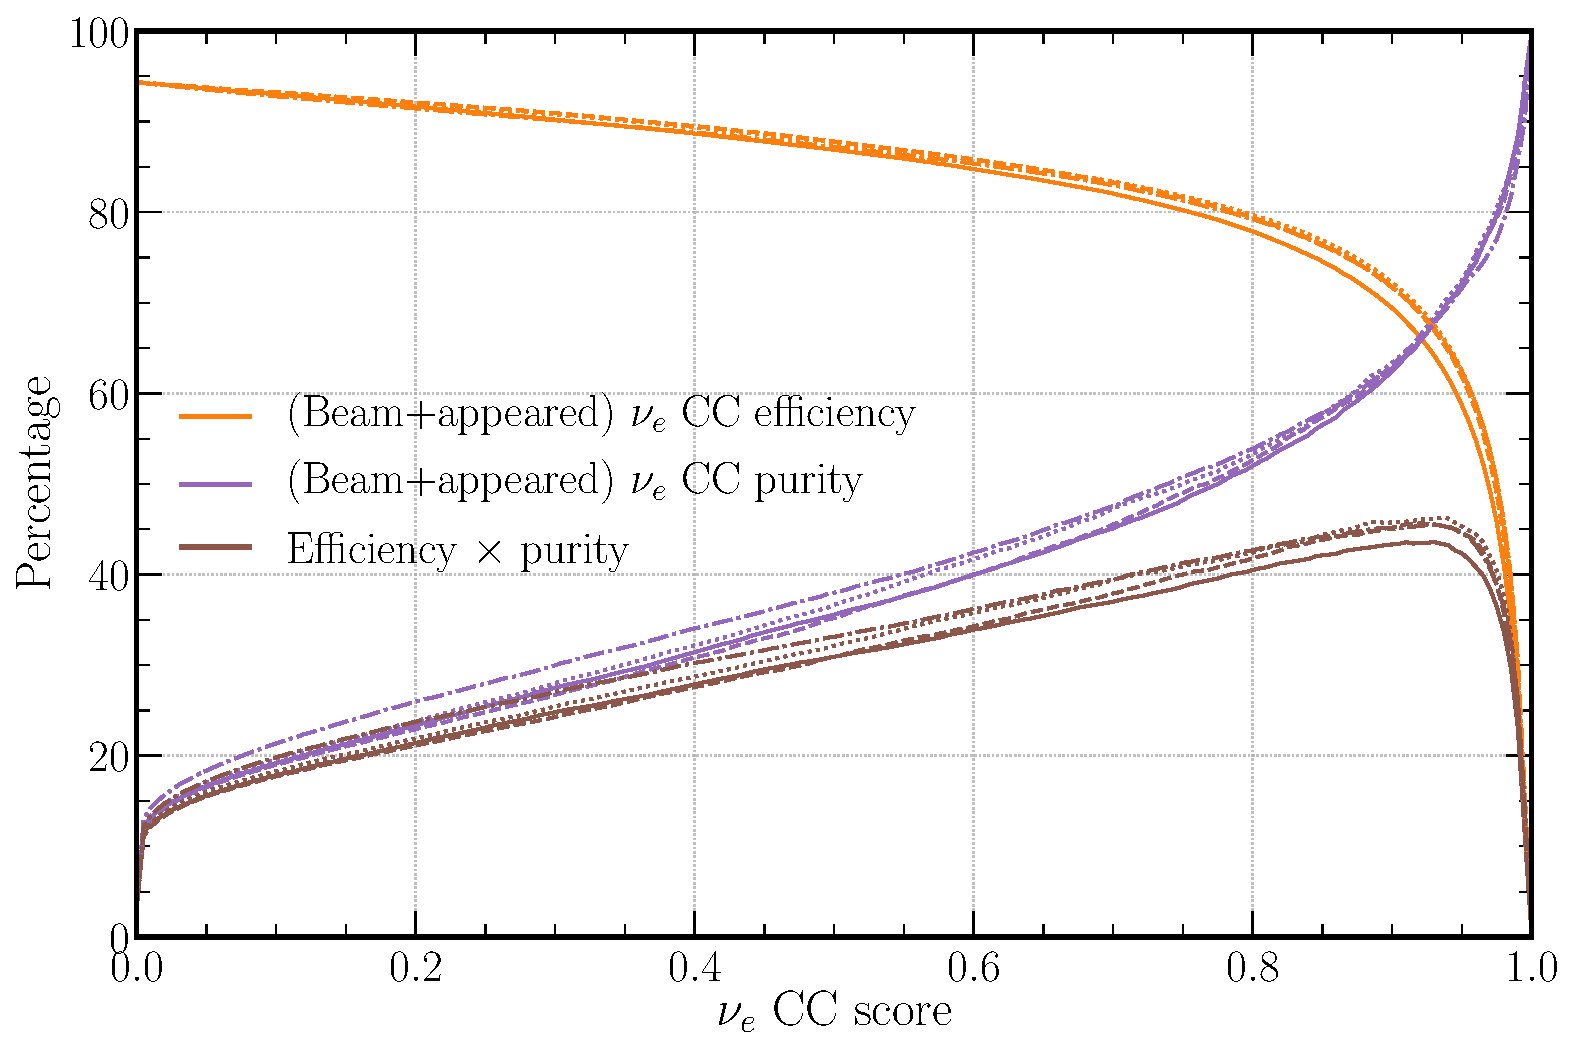
\includegraphics[width=0.6\textwidth]{diagrams/7-cvn/chipsnet/channel_nuel_eff_curves.pdf}
    \caption[channel nuel eff curves short]
    {c=solid, ct=dashed, cth=dotted, cth-stacked=dot-dash}
    \label{fig:channel_nuel_eff_curves}
\end{figure}

\begin{figure} % CHANNEL NUEL COMP CURVES DIAGRAM %
    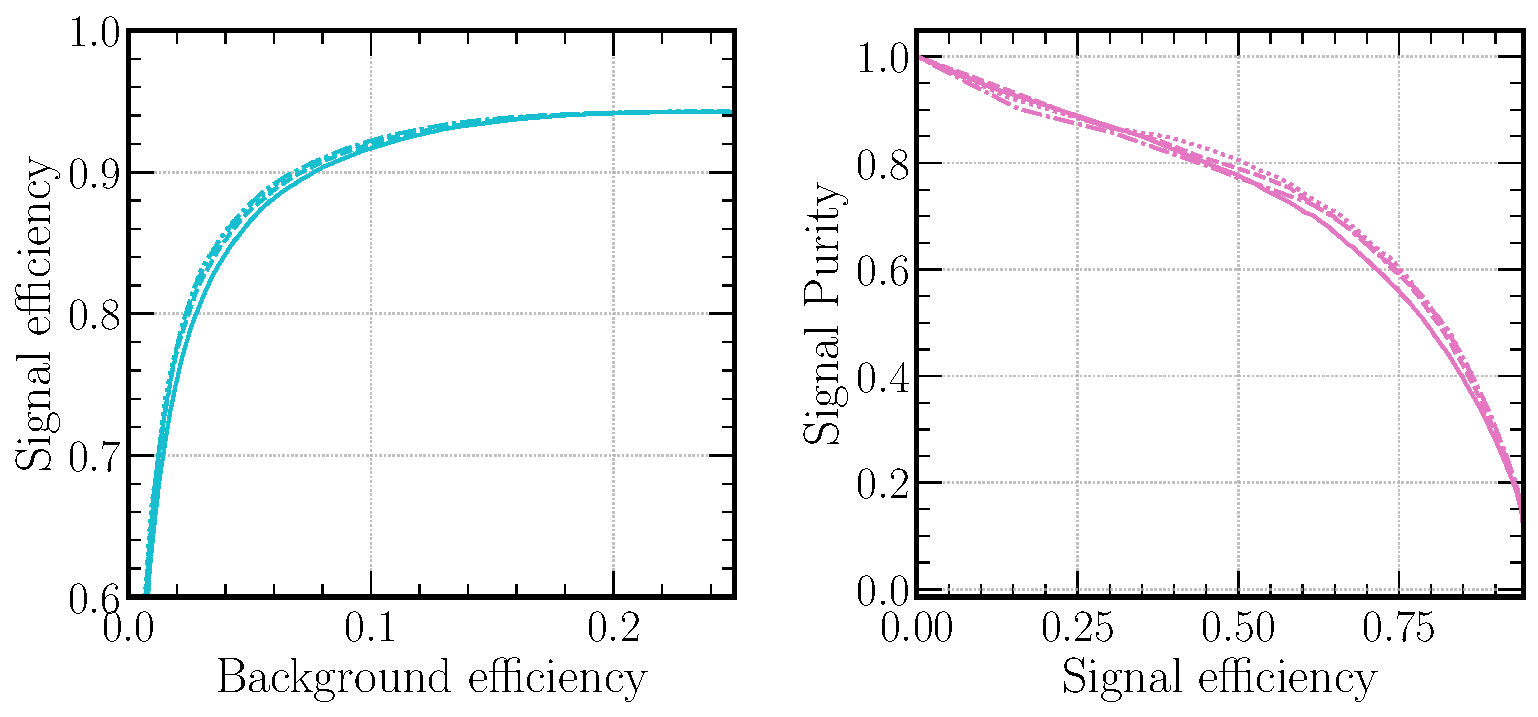
\includegraphics[width=0.8\textwidth]{diagrams/7-cvn/chipsnet/channel_nuel_comp_curves.pdf}
    \caption[channel nuel comp curves short]
    {c=solid, ct=dashed, cth=dotted, cth-stacked=dot-dash}
    \label{fig:channel_nuel_comp_curves}
\end{figure}

- Nuel-> ROC-AUC: 0.82377, PRC-AUC: 0.68935, S-Eff: 0.86860, S-Pur: 0.35681
- FOM1-> 0.43601, 0.91000, 53.71070, 12.22704, 17.60798, 0.67821, 0.64289
- FOM2-> 12.70378, 0.99000, 20.73912, 0.76294, 1.90217, 0.26187, 0.88613

- Nuel-> ROC-AUC: 0.82509, PRC-AUC: 0.70686, S-Eff: 0.87786, S-Pur: 0.35433
- FOM1-> 0.46118, 0.93000, 52.98765, 8.61419, 15.27335, 0.66908, 0.68927
- FOM2-> 13.26595, 0.98500, 29.74203, 1.43964, 3.58684, 0.37556, 0.85543

- Nuel-> ROC-AUC: 0.82559, PRC-AUC: 0.71155, S-Eff: 0.87661, S-Pur: 0.36928
- FOM1-> 0.46510, 0.93000, 53.44422, 8.34671, 15.75487, 0.67485, 0.68920
- FOM2-> 13.44645, 0.98500, 31.21664, 1.57028, 3.81933, 0.39418, 0.85277

- Nuel-> ROC-AUC: 0.82521, PRC-AUC: 0.70198, S-Eff: 0.87180, S-Pur: 0.38254
- FOM1-> 0.45819, 0.91500, 55.18628, 11.56662, 17.17741, 0.69684, 0.65753
- FOM2-> 12.66558, 0.99000, 24.37959, 1.35104, 2.35408, 0.30784, 0.86807

\begin{figure} % CHANNEL NUMU EFF CURVES DIAGRAM %
    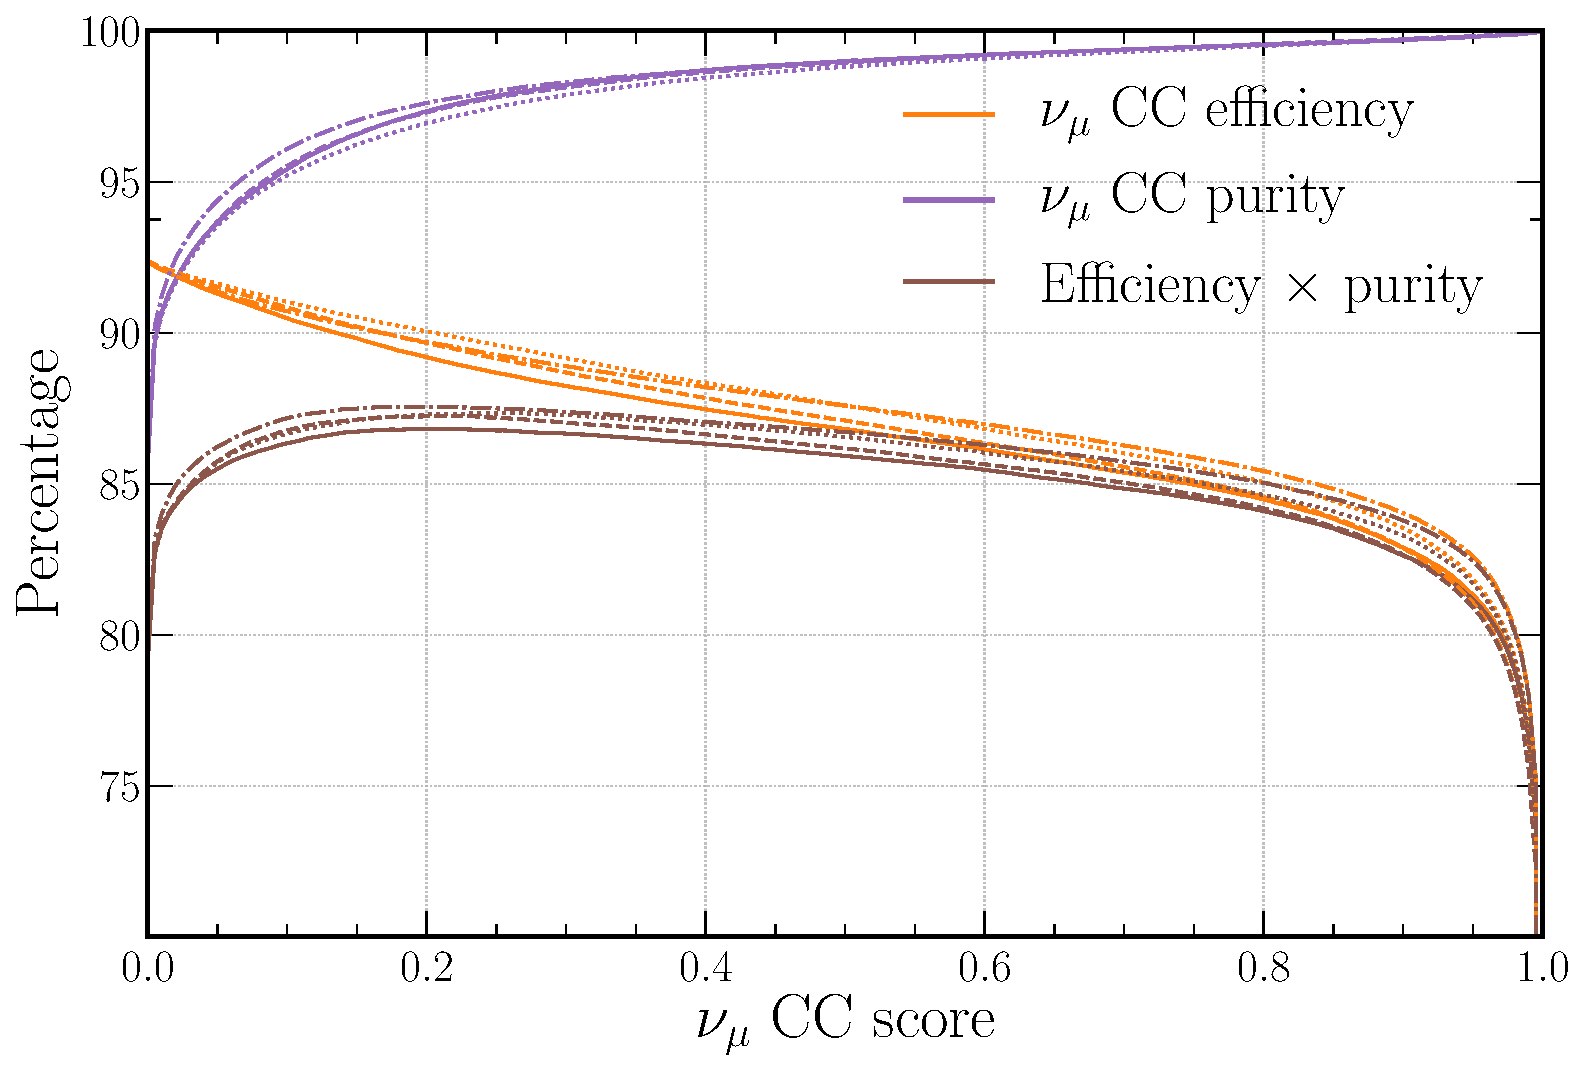
\includegraphics[width=0.6\textwidth]{diagrams/7-cvn/chipsnet/channel_numu_eff_curves.pdf}
    \caption[channel numu eff curves short]
    {c=solid, ct=dashed, cth=dotted, cth-stacked=dot-dash}
    \label{fig:channel_numu_eff_curves}
\end{figure}

\begin{figure} % CHANNEL NUMU COMP CURVES DIAGRAM %
    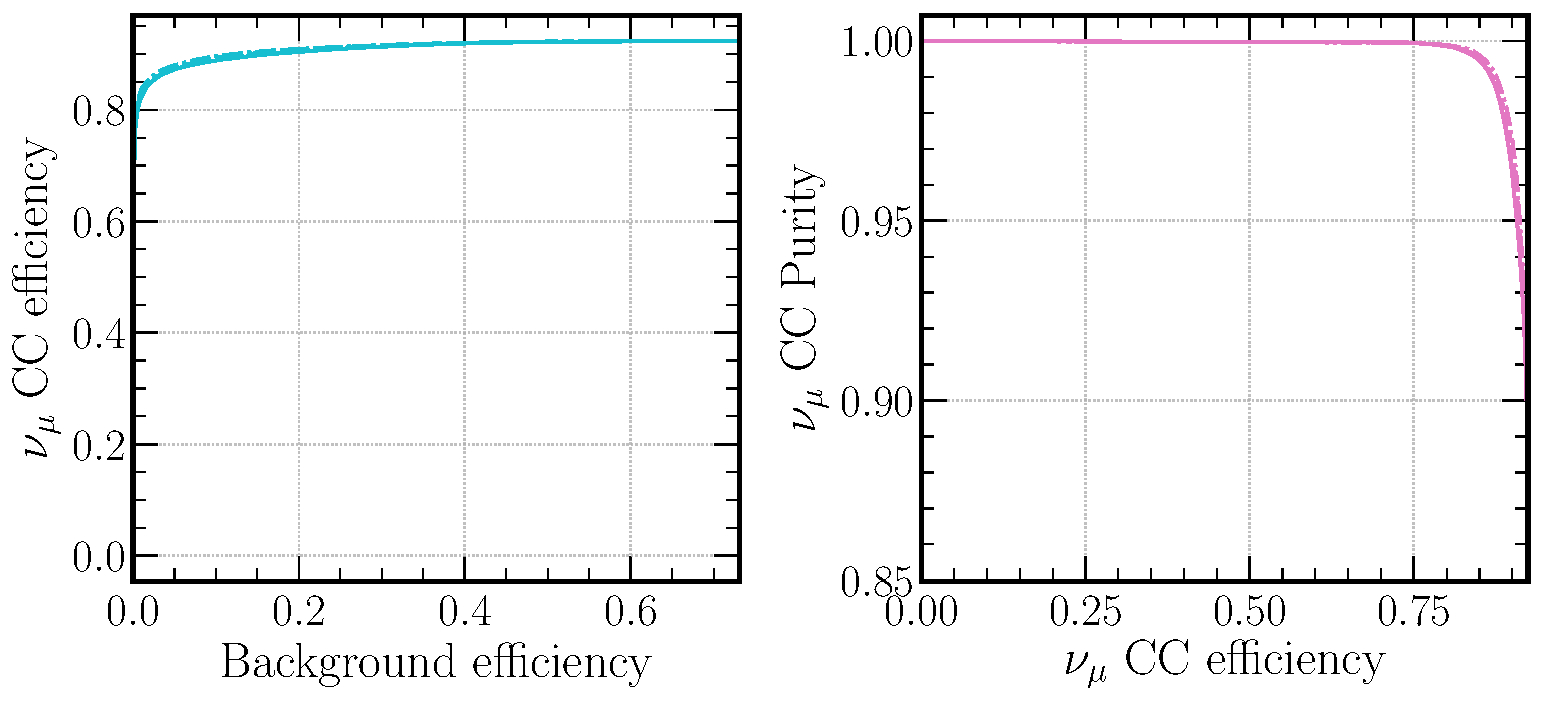
\includegraphics[width=0.8\textwidth]{diagrams/7-cvn/chipsnet/channel_numu_comp_curves.pdf}
    \caption[channel numu comp curves short]
    {c=solid, ct=dashed, cth=dotted, cth-stacked=dot-dash}
    \label{fig:channel_numu_comp_curves}
\end{figure}

\subsection{Multitask methodology} %%%%%%%%%%%%%%%%%%%%%%%%%%%%%%%%%%%%%%%%%%%%%%%%%%%%%%%%%%%%%%%
\label{sec:cvn_baseline_multi} %%%%%%%%%%%%%%%%%%%%%%%%%%%%%%%%%%%%%%%%%%%%%%%%%%%%%%%%%%%%%%%%%%%

Multi-task learning how to weight paper in Ref.~\cite{kendall2018}

\section{Cosmic muon rejection} %%%%%%%%%%%%%%%%%%%%%%%%%%%%%%%%%%%%%%%%%%%%%%%%%%%%%%%%%%%%%%%%%%
\label{sec:cvn_cosmic} %%%%%%%%%%%%%%%%%%%%%%%%%%%%%%%%%%%%%%%%%%%%%%%%%%%%%%%%%%%%%%%%%%%%%%%%%%%

\section{Beam classification} %%%%%%%%%%%%%%%%%%%%%%%%%%%%%%%%%%%%%%%%%%%%%%%%%%%%%%%%%%%%%%%%%%%%
\label{sec:cvn_beam} %%%%%%%%%%%%%%%%%%%%%%%%%%%%%%%%%%%%%%%%%%%%%%%%%%%%%%%%%%%%%%%%%%%%%%%%%%%%%

\subsection{Which categorisation to use} %%%%%%%%%%%%%%%%%%%%%%%%%%%%%%%%%%%%%%%%%%%%%%%%%%%%%%%%%
\label{sec:cvn_beam_cat} %%%%%%%%%%%%%%%%%%%%%%%%%%%%%%%%%%%%%%%%%%%%%%%%%%%%%%%%%%%%%%%%%%%%%%%%%

\begin{figure} % T_ALL_CAT SAMPLE DIAGRAM %
    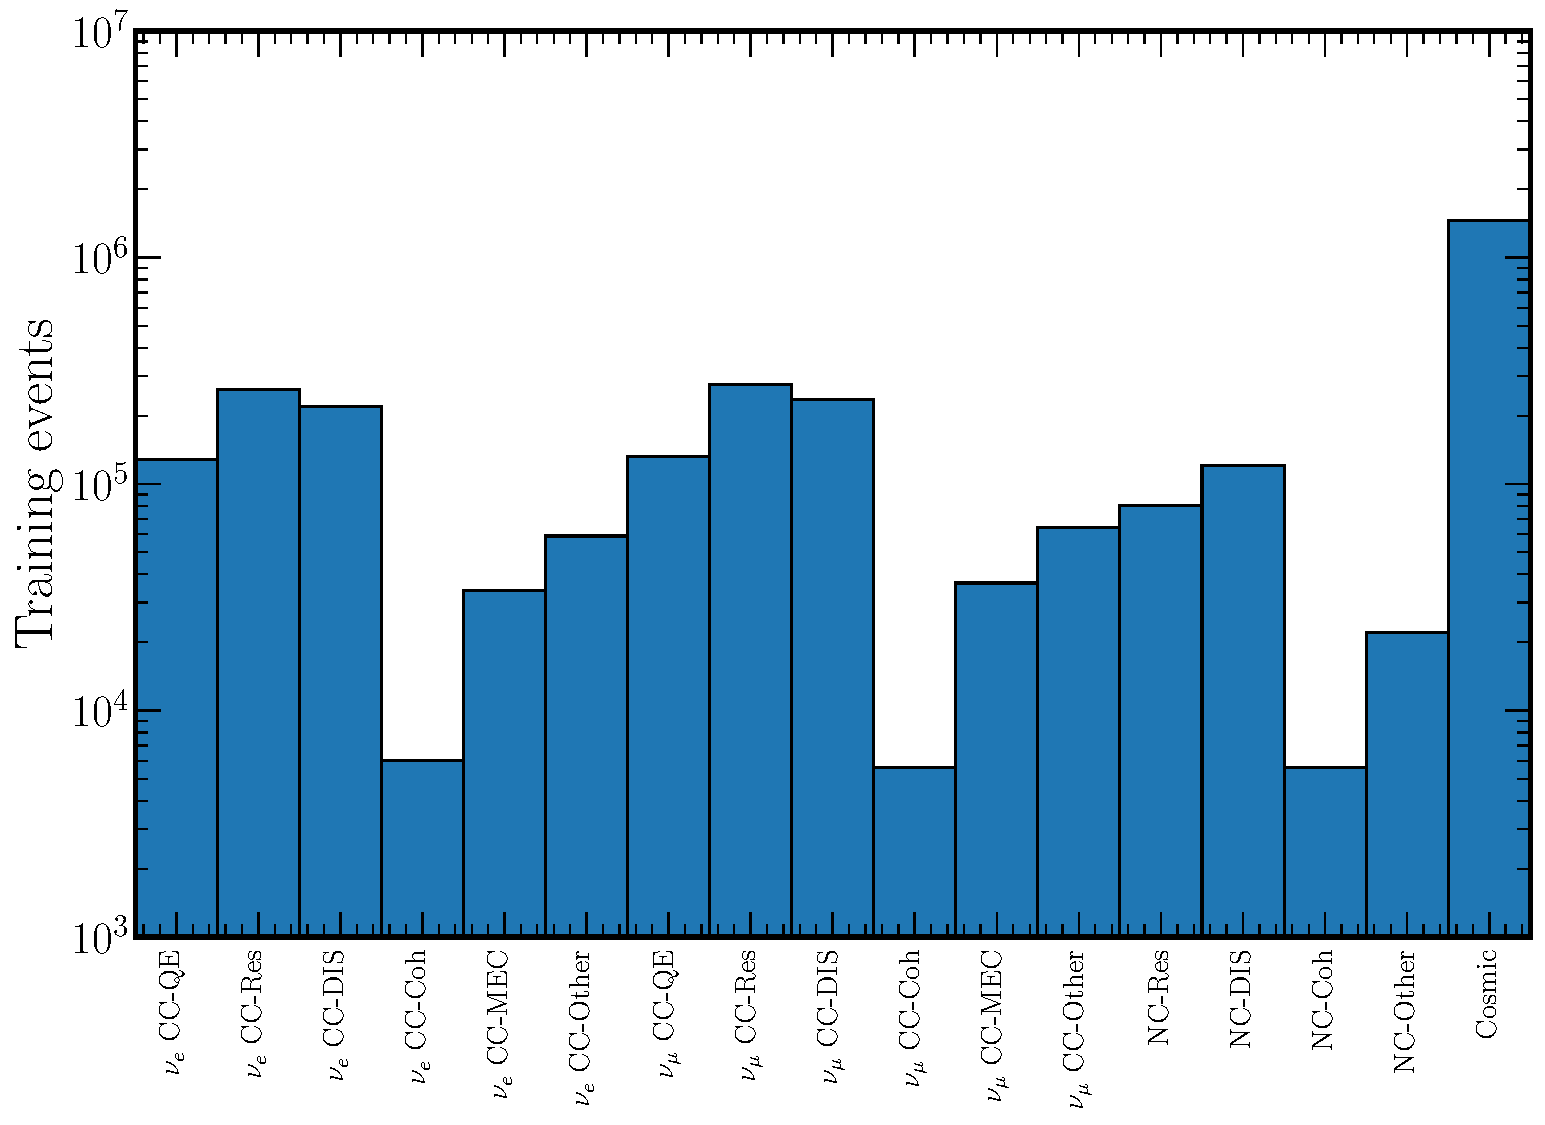
\includegraphics[width=0.6\textwidth]{diagrams/7-cvn/chipsnet/explore_t_all_cat.pdf}
    \caption[explore t all cat short]
    {explore t all cat long}
    \label{fig:explore_t_all_cat}
\end{figure}

\begin{figure} % T_NC_COMB_CAT SAMPLE DIAGRAM %
    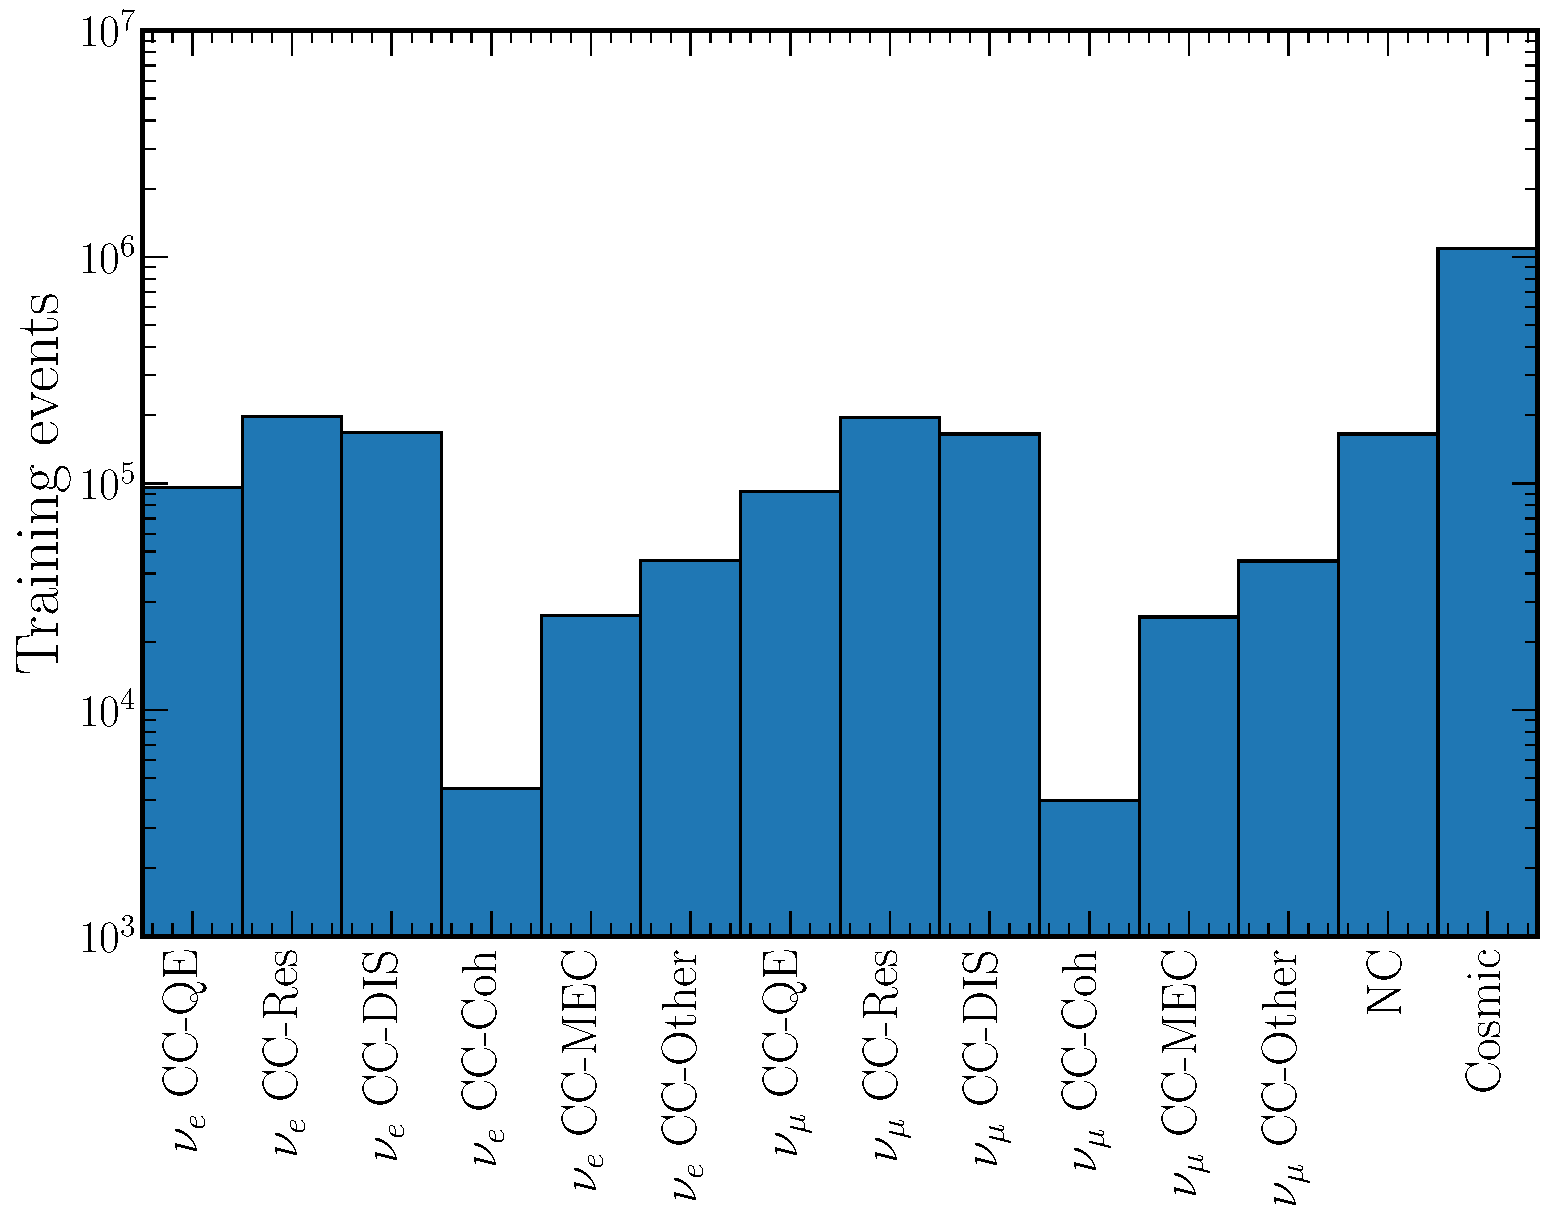
\includegraphics[width=0.6\textwidth]{diagrams/7-cvn/chipsnet/explore_t_nc_comb_cat.pdf}
    \caption[explore t nc comb cat short]
    {explore t nc comb cat long}
    \label{fig:explore_t_nc_comb_cat}
\end{figure}

\begin{figure} % T_COMB_CAT SAMPLE DIAGRAM %
    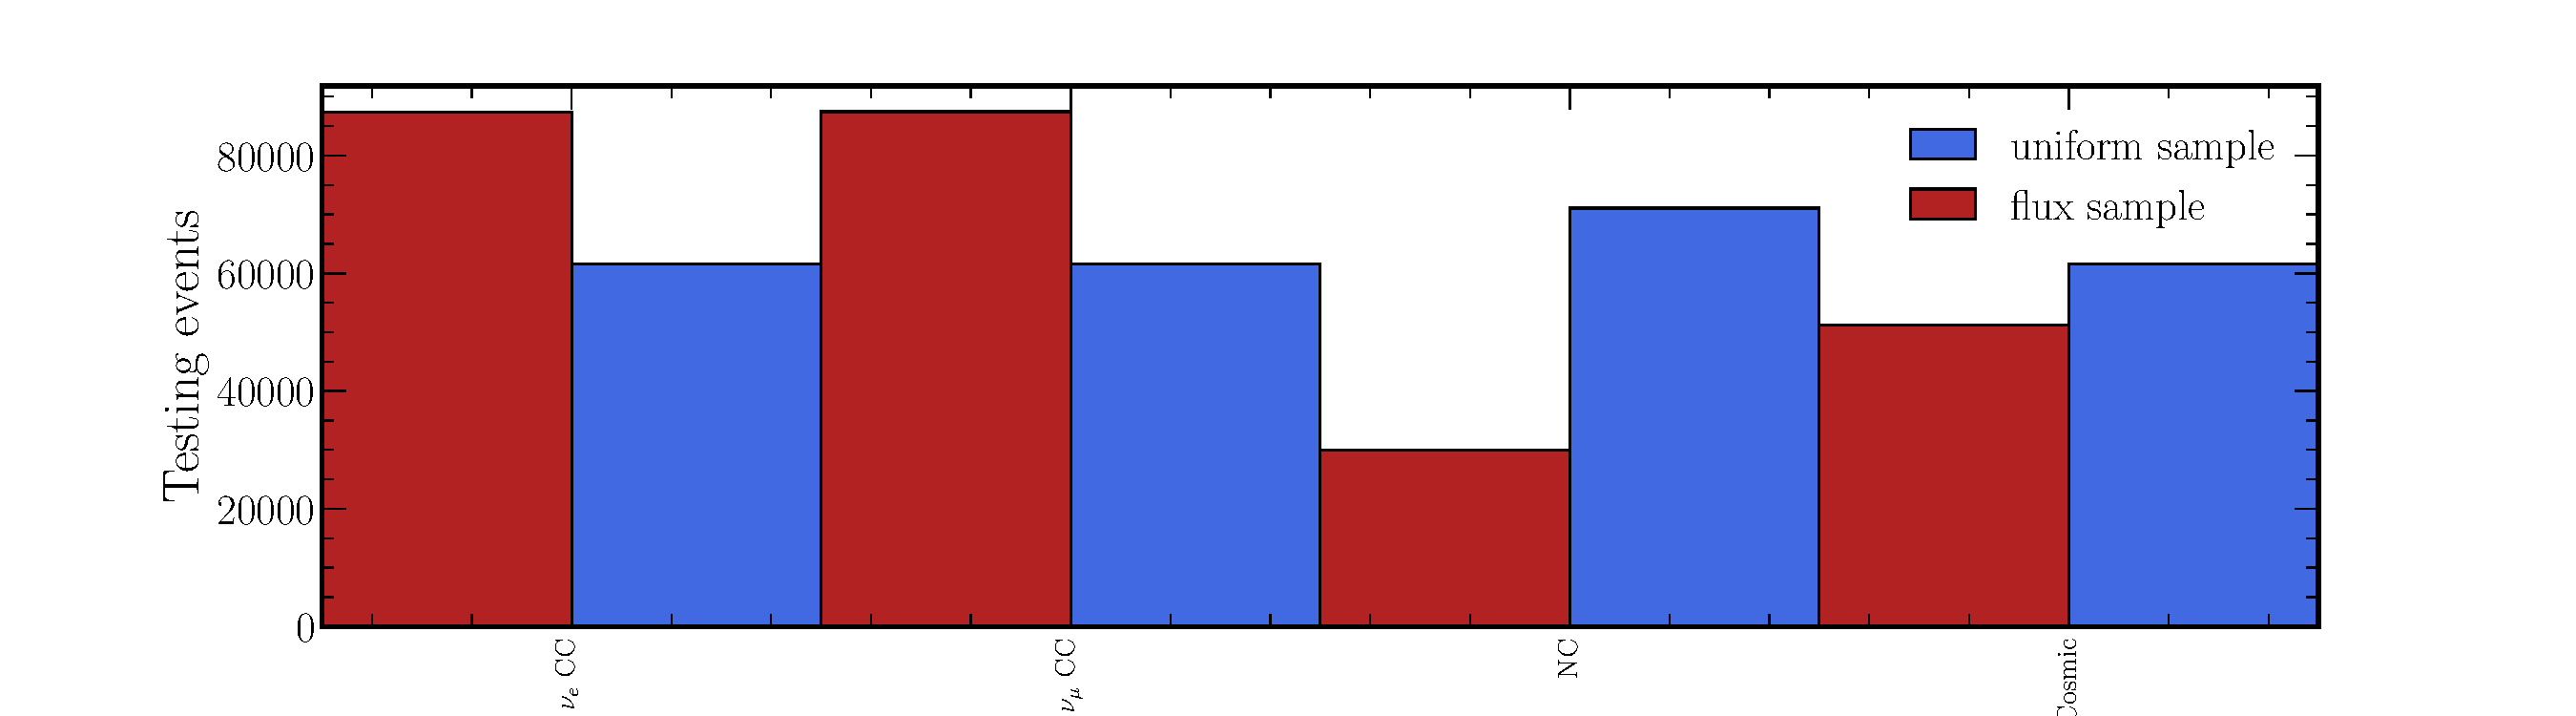
\includegraphics[width=0.6\textwidth]{diagrams/7-cvn/chipsnet/explore_t_comb_cat.pdf}
    \caption[explore t comb cat short]
    {explore t comb cat long}
    \label{fig:explore_t_comb_cat}
\end{figure}

\begin{figure} % CAT NUEL EFF CURVES DIAGRAM %
    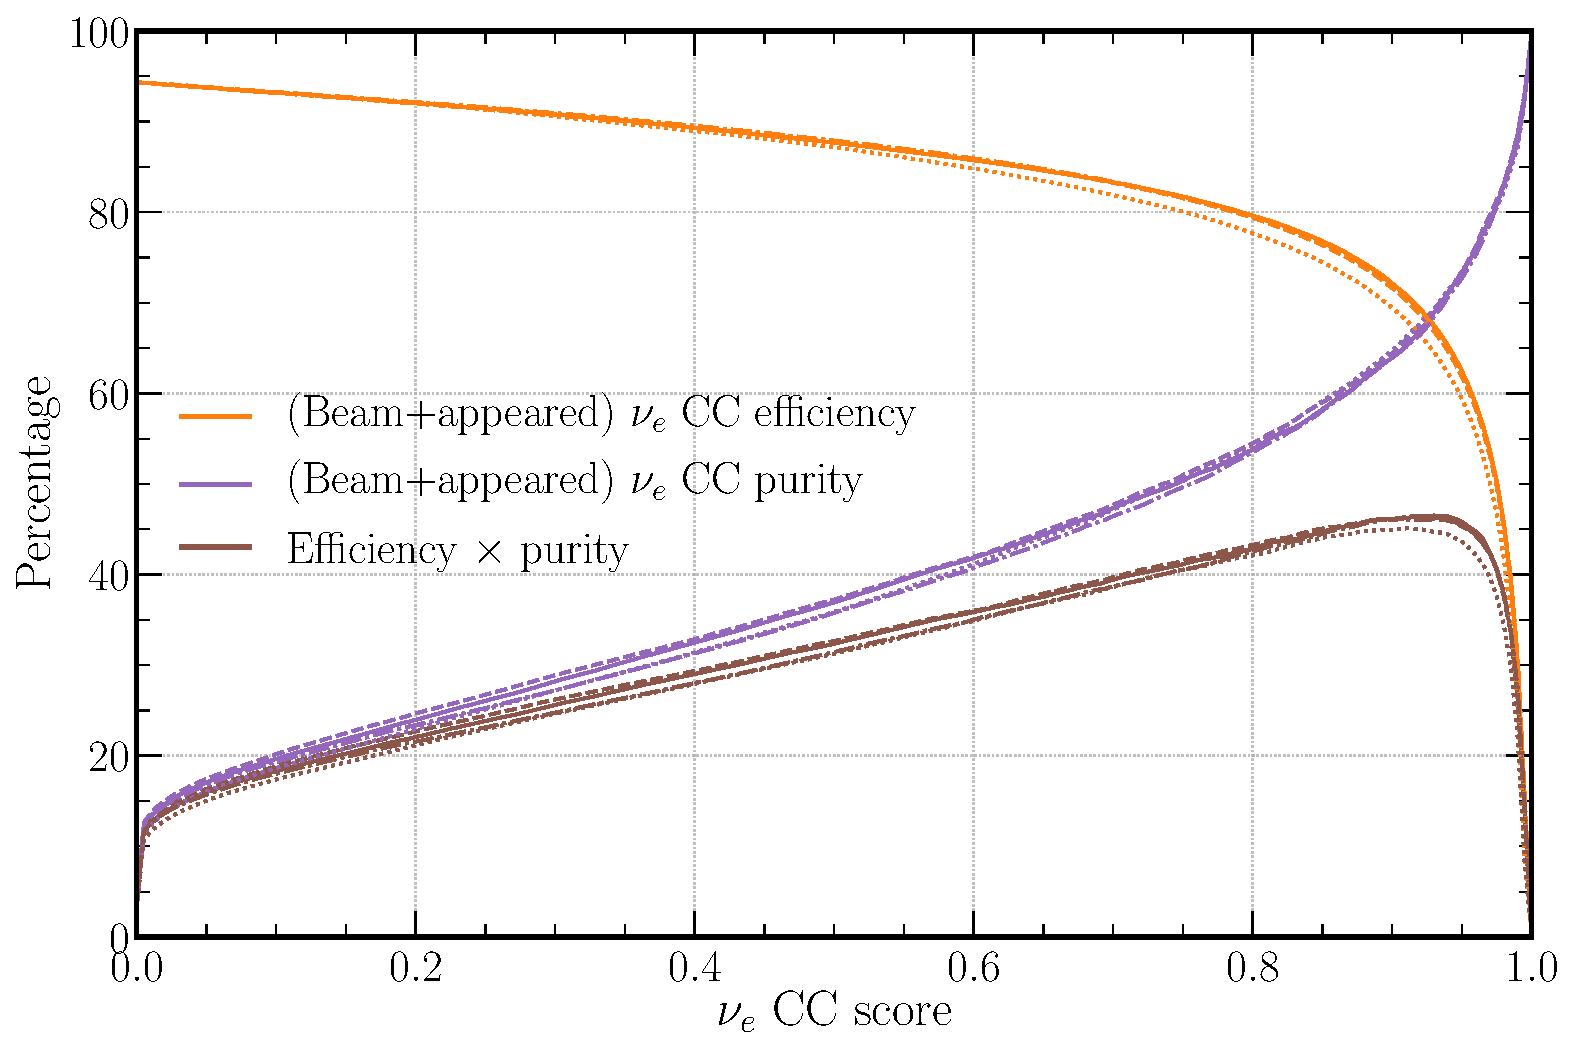
\includegraphics[width=0.6\textwidth]{diagrams/7-cvn/chipsnet/cat_nuel_eff_curves.pdf}
    \caption[cat nuel eff curves short]
    {cat nuel eff curves long}
    \label{fig:cat_nuel_eff_curves}
\end{figure}

\begin{figure} % CAT NUEL COMP CURVES DIAGRAM %
    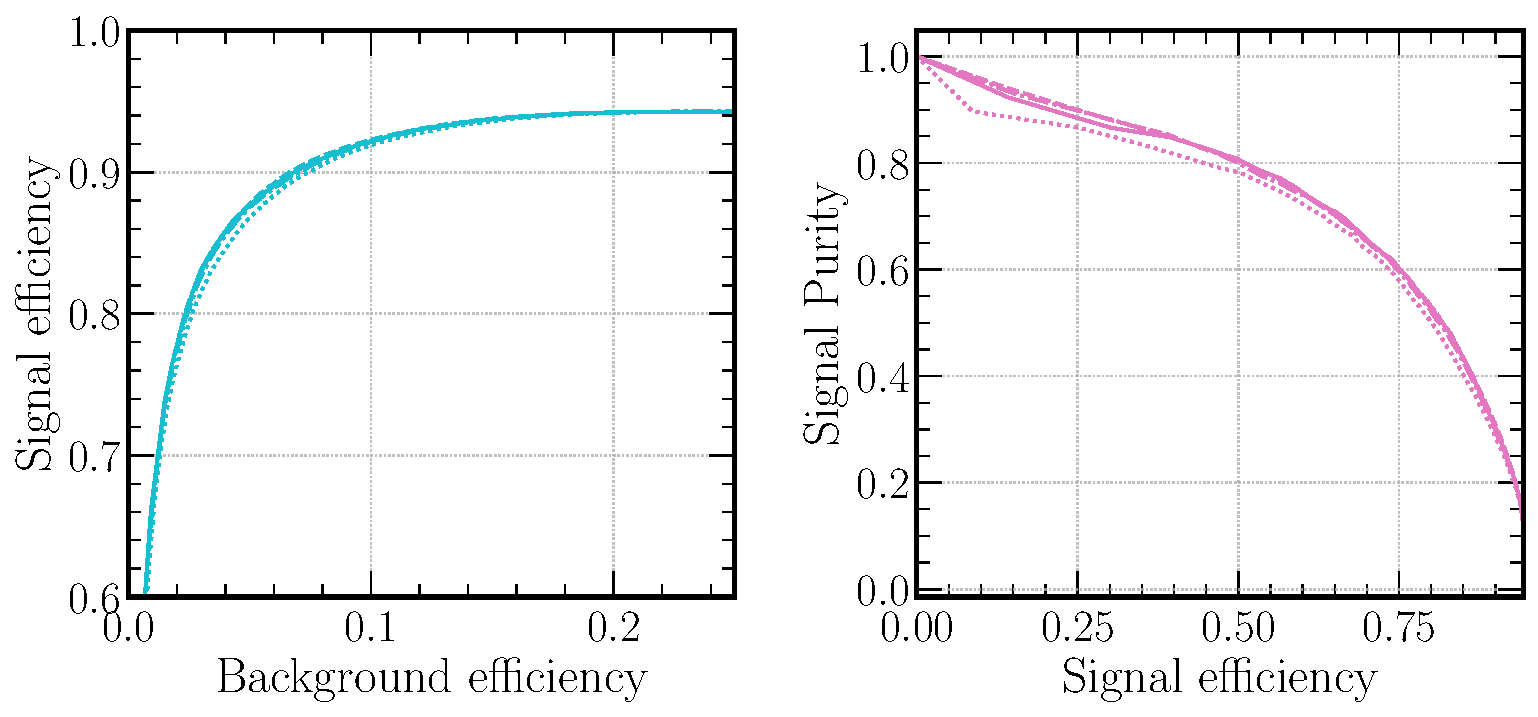
\includegraphics[width=0.8\textwidth]{diagrams/7-cvn/chipsnet/cat_nuel_comp_curves.pdf}
    \caption[cat nuel comp curves short]
    {cat nuel comp curves long}
    \label{fig:cat_nuel_comp_curves}
\end{figure}

\begin{figure} % CAT NUMU EFF CURVES DIAGRAM %
    \includegraphics[width=0.6\textwidth]{diagrams/7-cvn/chipsnet/cat_numu_eff_curves.pdf}
    \caption[cat numu eff curves short]
    {cat numu eff curves long}
    \label{fig:cat_numu_eff_curves}
\end{figure}

\begin{figure} % CAT NUMU COMP CURVES DIAGRAM %
    \includegraphics[width=0.8\textwidth]{diagrams/7-cvn/chipsnet/cat_numu_comp_curves.pdf}
    \caption[cat numu comp curves short]
    {cat numu comp curves long}
    \label{fig:cat_numu_comp_curves}
\end{figure}

\subsection{Does counting primary particles help?} %%%%%%%%%%%%%%%%%%%%%%%%%%%%%%%%%%%%%%%%%%%%%%%
\label{sec:cvn_beam_prim} %%%%%%%%%%%%%%%%%%%%%%%%%%%%%%%%%%%%%%%%%%%%%%%%%%%%%%%%%%%%%%%%%%%%%%%%

\begin{figure} % BEAM NUEL EFF CURVES DIAGRAM %
    \includegraphics[width=0.6\textwidth]{diagrams/7-cvn/chipsnet/beam_nuel_eff_curves.pdf}
    \caption[beam nuel eff curves short]
    {beam nuel eff curves long}
    \label{fig:beam_nuel_eff_curves}
\end{figure}

\begin{figure} % BEAM NUEL COMP CURVES DIAGRAM %
    \includegraphics[width=0.8\textwidth]{diagrams/7-cvn/chipsnet/beam_nuel_comp_curves.pdf}
    \caption[beam nuel comp curves short]
    {beam nuel comp curves long}
    \label{fig:beam_nuel_comp_curves}
\end{figure}

\begin{figure} % BEAM NUMU EFF CURVES DIAGRAM %
    \includegraphics[width=0.6\textwidth]{diagrams/7-cvn/chipsnet/beam_numu_eff_curves.pdf}
    \caption[beam numu eff curves short]
    {beam numu eff curves long}
    \label{fig:beam_numu_eff_curves}
\end{figure}

\begin{figure} % BEAM NUMU COMP CURVES DIAGRAM %
    \includegraphics[width=0.8\textwidth]{diagrams/7-cvn/chipsnet/beam_numu_comp_curves.pdf}
    \caption[beam numu comp curves short]
    {beam numu comp curves long}
    \label{fig:beam_numu_comp_curves}
\end{figure}

\section{Energy estimation} %%%%%%%%%%%%%%%%%%%%%%%%%%%%%%%%%%%%%%%%%%%%%%%%%%%%%%%%%%%%%%%%%%%%%%
\label{sec:cvn_energy} %%%%%%%%%%%%%%%%%%%%%%%%%%%%%%%%%%%%%%%%%%%%%%%%%%%%%%%%%%%%%%%%%%%%%%%%%%%

\subsection{Neutrino and lepton multitask} %%%%%%%%%%%%%%%%%%%%%%%%%%%%%%%%%%%%%%%%%%%%%%%%%%%%%%%
\label{sec:cvn_energy_chan} %%%%%%%%%%%%%%%%%%%%%%%%%%%%%%%%%%%%%%%%%%%%%%%%%%%%%%%%%%%%%%%%%%%%%%

\begin{figure} % ENERGY CHAN DISTS DIAGRAM %
    \includegraphics[width=\textwidth]{diagrams/7-cvn/chipsnet/energy_chan_frac_dist.pdf}
    \caption[energy chan frac dist short]
    {energy chan frac dist long}
    \label{fig:energy_chan_frac_dist}
\end{figure}

\begin{figure} % ENERGY CHAN FRAC VS E DIAGRAM %
    \includegraphics[width=\textwidth]{diagrams/7-cvn/chipsnet/energy_chan_frac_vs_e.pdf}
    \caption[energy chan frac vs e short]
    {energy chan frac vs e long}
    \label{fig:energy_chan_frac_vs_e}
\end{figure}

\subsection{Extra parameters} %%%%%%%%%%%%%%%%%%%%%%%%%%%%%%%%%%%%%%%%%%%%%%%%%%%%%%%%%%%%%%%%%%%%
\label{sec:cvn_energy_par} %%%%%%%%%%%%%%%%%%%%%%%%%%%%%%%%%%%%%%%%%%%%%%%%%%%%%%%%%%%%%%%%%%%%%%%

\begin{figure} % ENERGY PAR DISTS DIAGRAM %
    \includegraphics[width=\textwidth]{diagrams/7-cvn/chipsnet/energy_par_frac_dist.pdf}
    \caption[energy par frac dist short]
    {energy par frac dist long}
    \label{fig:energy_par_frac_dist}
\end{figure}

\begin{figure} % ENERGY PAR FRAC VS E DIAGRAM %
    \includegraphics[width=\textwidth]{diagrams/7-cvn/chipsnet/energy_par_frac_vs_e.pdf}
    \caption[energy par frac vs e short]
    {energy par frac vs e long}
    \label{fig:energy_par_frac_vs_e}
\end{figure}

\subsection{Combined or split} %%%%%%%%%%%%%%%%%%%%%%%%%%%%%%%%%%%%%%%%%%%%%%%%%%%%%%%%%%%%%%%%%%%
\label{sec:cvn_energy_split} %%%%%%%%%%%%%%%%%%%%%%%%%%%%%%%%%%%%%%%%%%%%%%%%%%%%%%%%%%%%%%%%%%%%%

\begin{figure} % ENERGY SPLIT NUEL DIAGRAM %
    \includegraphics[width=\textwidth]{diagrams/7-cvn/chipsnet/final_energy_split_nuel_frac_vs_e.pdf}
    \caption[final energy split nuel frac vs e short]
    {final energy split nuel frac vs e long}
    \label{fig:final_energy_split_nuel_frac_vs_e}
\end{figure}

\begin{figure} % ENERGY SPLIT NUMU DIAGRAM %
    \includegraphics[width=\textwidth]{diagrams/7-cvn/chipsnet/final_energy_split_numu_frac_vs_e.pdf}
    \caption[final energy split numu frac vs e short]
    {final energy split numu frac vs e long}
    \label{fig:final_energy_split_numu_frac_vs_e}
\end{figure}

\section{Combined performance} %%%%%%%%%%%%%%%%%%%%%%%%%%%%%%%%%%%%%%%%%%%%%%%%%%%%%%%%%%%%%%%%%%%
\label{sec:cvn_final} %%%%%%%%%%%%%%%%%%%%%%%%%%%%%%%%%%%%%%%%%%%%%%%%%%%%%%%%%%%%%%%%%%%%%%%%%%%%

\begin{figure} % COSMIC HISTORY DIAGRAM %
    \includegraphics[width=0.6\textwidth]{diagrams/7-cvn/chipsnet/final_cosmic_history.pdf}
    \caption[final cosmic history short]
    {final cosmic history long}
    \label{fig:final_cosmic_history}
\end{figure}

\begin{figure} % BEAM HISTORY DIAGRAM %
    \includegraphics[width=0.6\textwidth]{diagrams/7-cvn/chipsnet/final_beam_history.pdf}
    \caption[final beam history short]
    {final beam history long}
    \label{fig:final_beam_history}
\end{figure}

\begin{figure} % ENERGY HISTORY DIAGRAM %
    \includegraphics[width=0.6\textwidth]{diagrams/7-cvn/chipsnet/final_energy_history.pdf}
    \caption[final energy history short]
    {final energy history long}
    \label{fig:final_energy_history}
\end{figure}

\begin{figure} % COSMIC OUTPUTS DIAGRAM %
    \includegraphics[width=0.6\textwidth]{diagrams/7-cvn/chipsnet/final_cosmic_outputs.pdf}
    \caption[final cosmic outputs short]
    {final cosmic outputs long}
    \label{fig:final_cosmic_outputs}
\end{figure}

\begin{figure} % COSMIC OUTPUTS ZOOMED DIAGRAM %
    \includegraphics[width=0.6\textwidth]{diagrams/7-cvn/chipsnet/final_cosmic_zoomed_outputs.pdf}
    \caption[final cosmic zoomed outputs short]
    {final cosmic zoomed outputs long}
    \label{fig:final_cosmic_zoomed_outputs}
\end{figure}

\begin{figure} % ESCAPES OUTPUTS DIAGRAM %
    \includegraphics[width=0.6\textwidth]{diagrams/7-cvn/chipsnet/final_escapes_outputs.pdf}
    \caption[final escapes outputs short]
    {final escapes outputs long}
    \label{fig:final_escapes_outputs}
\end{figure}

\begin{figure} % BEAM OUTPUTS NUEL DIAGRAM %
    \includegraphics[width=0.6\textwidth]{diagrams/7-cvn/chipsnet/final_beam_nuel_outputs.pdf}
    \caption[final beam nuel outputs short]
    {final beam nuel outputs long}
    \label{fig:final_beam_nuel_outputs}
\end{figure}

\begin{figure} % BEAM OUTPUTS NUMU DIAGRAM %
    \includegraphics[width=0.6\textwidth]{diagrams/7-cvn/chipsnet/final_beam_numu_outputs.pdf}
    \caption[final beam numu outputs short]
    {final beam numu outputs long}
    \label{fig:final_beam_numu_outputs}
\end{figure}

\begin{figure} % FINAL NUEL EFF CURVES DIAGRAM %
    \includegraphics[width=0.6\textwidth]{diagrams/7-cvn/chipsnet/final_nuel_eff_curves.pdf}
    \caption[final nuel eff curves short]
    {final nuel eff curves long}
    \label{fig:final_nuel_eff_curves}
\end{figure}

\begin{figure} % FINAL NUMU EFF CURVES DIAGRAM %
    \includegraphics[width=0.6\textwidth]{diagrams/7-cvn/chipsnet/final_numu_eff_curves.pdf}
    \caption[final numu eff curves short]
    {final numu eff curves long}
    \label{fig:final_numu_eff_curves}
\end{figure}

\begin{figure} % FINAL NUEL HISTS DIAGRAM %
    \includegraphics[width=0.6\textwidth]{diagrams/7-cvn/chipsnet/final_nuel_hists.pdf}
    \caption[final nuel hists short]
    {final nuel hists long}
    \label{fig:final_nuel_hists}
\end{figure}

\begin{figure} % FINAL NUMU HISTS DIAGRAM %
    \includegraphics[width=0.6\textwidth]{diagrams/7-cvn/chipsnet/final_numu_hists.pdf}
    \caption[final numu hists short]
    {final numu hists long}
    \label{fig:final_numu_hists}
\end{figure}

\begin{figure} % FINAL COMB CAT CONFUSION DIAGRAM %
    \includegraphics[width=0.6\textwidth]{diagrams/7-cvn/chipsnet/final_comb_cat_confusion.pdf}
    \caption[final comb cat confusion short]
    {final comb cat confusion long}
    \label{fig:final_comb_cat_confusion}
\end{figure}

\begin{figure} % FINAL CC CAT CONFUSION DIAGRAM %
    \includegraphics[width=0.6\textwidth]{diagrams/7-cvn/chipsnet/final_cc_cat_confusion.pdf}
    \caption[final cc cat confusion short]
    {final cc cat confusion long}
    \label{fig:final_cc_cat_confusion}
\end{figure}

\begin{figure} % FINAL NC CAT CONFUSION DIAGRAM %
    \includegraphics[width=0.6\textwidth]{diagrams/7-cvn/chipsnet/final_nc_cat_confusion.pdf}
    \caption[final nc cat confusion short]
    {final nc cat confusion long}
    \label{fig:final_nc_cat_confusion}
\end{figure}

\begin{figure} % FINAL NUEL ENERGY DIST DIAGRAM %
    \includegraphics[width=0.6\textwidth]{diagrams/7-cvn/chipsnet/final_nuel_passed_energy_dist.pdf}
    \caption[final nuel passed energy dist short]
    {final nuel passed energy dist long}
    \label{fig:final_nuel_passed_energy_dist}
\end{figure}

\begin{figure} % FINAL NUMU ENERGY DIST DIAGRAM %
    \includegraphics[width=0.6\textwidth]{diagrams/7-cvn/chipsnet/final_numu_passed_energy_dist.pdf}
    \caption[final numu passed energy dist short]
    {final numu passed energy dist long}
    \label{fig:final_numu_passed_energy_dist}
\end{figure}

\begin{figure} % FINAL 2D ENERGY DIAGRAM %
    \includegraphics[width=0.8\textwidth]{diagrams/7-cvn/chipsnet/final_energy_2d.pdf}
    \caption[final energy 2d short]
    {final energy 2d long}
    \label{fig:final_energy_2d}
\end{figure}

\begin{figure} % FINAL NUEL ENERGY DIAGRAM %
    \includegraphics[width=0.8\textwidth]{diagrams/7-cvn/chipsnet/final_energy_nuel.pdf}
    \caption[final energy nuel short]
    {final energy nuel long}
    \label{fig:final_energy_nuel}
\end{figure}

\begin{figure} % FINAL NUMU ENERGY DIAGRAM %
    \includegraphics[width=0.8\textwidth]{diagrams/7-cvn/chipsnet/final_energy_numu.pdf}
    \caption[final energy numu short]
    {final energy numu long}
    \label{fig:final_energy_numu}
\end{figure}

\section{Explainability} %%%%%%%%%%%%%%%%%%%%%%%%%%%%%%%%%%%%%%%%%%%%%%%%%%%%%%%%%%%%%%%%%%%%%%%%%
\label{sec:cvn_explain} %%%%%%%%%%%%%%%%%%%%%%%%%%%%%%%%%%%%%%%%%%%%%%%%%%%%%%%%%%%%%%%%%%%%%%%%%%

\begin{figure} % COSMIC t-SNE DIAGRAM %
    \includegraphics[width=0.8\textwidth]{diagrams/7-cvn/chipsnet/final_cosmic_tsne.pdf}
    \caption[final cosmic tsne short]
    {final cosmic tsne long}
    \label{fig:final_cosmic_tsne}
\end{figure}

\begin{figure} % BEAM t-SNE DIAGRAM %
    \includegraphics[width=0.8\textwidth]{diagrams/7-cvn/chipsnet/final_beam_tsne.pdf}
    \caption[final beam tsne short]
    {final beam tsne long}
    \label{fig:final_beam_tsne}
\end{figure}

\begin{figure} % BEAM t-SNE EVENTS DIAGRAM %
    \includegraphics[width=\textwidth]{diagrams/7-cvn/chipsnet/final_beam_tsne_events.pdf}
    \caption[final beam tsne events short]
    {final beam tsne events long}
    \label{fig:final_beam_tsne_events}
\end{figure}

\begin{figure} % FRAC ENERGY EFF DIAGRAM %
    \includegraphics[width=0.6\textwidth]{diagrams/7-cvn/chipsnet/final_frac_energy_eff.pdf}
    \caption[final frac energy eff short]
    {final frac energy eff long}
    \label{fig:final_frac_energy_eff}
\end{figure}

\begin{figure} % EXPLAIN EXAMPLE EVENT DIAGRAM %
    \includegraphics[width=\textwidth]{diagrams/7-cvn/chipsnet/explain_example_event.pdf}
    \caption[explain example event short]
    {explain example event long}
    \label{fig:explain_example_event}
\end{figure}

\begin{figure} % BEAGLEBONE AND DANOUT DIAGRAM %
    \centering
    \subcaptionbox{explain cosmic activations\label{fig:explain_cosmic_activations}}{%
        \includegraphics[height=16cm]{diagrams/7-cvn/chipsnet/explain_cosmic_activations.pdf}%
    }
    \quad
    \subcaptionbox{explain beam activations\label{fig:explain_beam_activations}}{%
        \includegraphics[height=16cm]{diagrams/7-cvn/chipsnet/explain_beam_activations.pdf}%
    }
    \quad
    \subcaptionbox{explain energy activations\label{fig:explain_energy_activations}}{%
        \includegraphics[height=16cm]{diagrams/7-cvn/chipsnet/explain_energy_activations.pdf}%
    }
    \caption[The caption]
    {The caption}
\end{figure}

Initial CNN visualisation paper in Ref.~\cite{zeiler2013}
Original t-SNE paper in Ref.~\cite{maaten2008}
Grad-CAM paper in Ref.~\cite{selvaraju2017}

- For all the t-SNE stuff
- There have been plently of attempts at visualising high-dimensional data on a 2/3 dimensional
map, including Sammon mapping, Isomap, Locally Linear Embedding, Stochastic Neighbour Embedding.
- Older implementations tended to cluster all data points towards the centre of the map and proved
difficult to optimise.
- You basically set a summed probability between all points in the low-dimensional space to a
summed probability between all points in the high-dimensional space.
- t-SNE uses the student-t distribution (with a heavy tail) in the low-dimensional space to
calculate the probability. This alleviates both the crowding problem and is easier to optimise.
- Optimisation uses a simple momentum term, plus two new ideas. "Early compression" which forces
map points to stay close to each other at the start of optimisation, it is then easier for
clusters to move through each other and explore all possible global organisations of the data,
this is implemented as an L2-penalty term proportional to the sum of squared distances from the
origin, this is then removed at an iteration given as input. Secondly, "Early exaggeration" which
creates tight widely seperated clusters.

TODO: Sort everything below!!!!

- Take insights from neuroscience. The human eye can do remarkably well at image recognition, even neutrino event classification if
you know what to look for. But we will have way too much data, so need to train a computer to do this task for us.
- A MPL with a single hidden layer can be shown to apprximate any function arbitrarily accurately. Give REF for this.
- Conv is a set of 'filters' that when applied via scanning across an input image result in a feature map
- Pooling used as each layer requires less complexity and it is less important about the location and that the feature exists.
- Few learners search their hypothesis space fully. Therefore, a learner with a large hypothesis space that tries fewer hypotheses from it is less likely to overfit than one that tries more hypotheses from a smaller space.
- All that "deep" really means is just many many hidden layers, which can encode complex structures more efficienctly.
- They can be very difficult to train, but with GPUs, bigger training sets, weight inits, better non linearities, SGD, prevention of overfitting techniques and conv networks, its possible.

- We do not predefine the filters, they are also trained to extact the important features from the event images
- Approaches in the past for event classification using CNNs for water cherenkov detectors have taken a few Approaches to generating the input image representation.
- Projecting onto a 2d surface "outside" the detector

- Primary goal is to classify the neutrino flavour nuel CC, numu CC or NC
- Secondary goal is to then classify the individual interaction mode (QEL, RES, DIS etc...) these will have different energy resolutions and systematic uncertainties, so seperation can provide increased sensitivity.
- See signal interactions peaked closely near score values of unity and the backgrounds lie close to the zero score as expected.
- DUNE chose their selection cut to maximise the oscillation analysis sensitivity, determining sin(delta-cp) != 0
- Can choose many different output configurations/categorisations for the events.
- Should you combined into a big list of categories, should you combine the NC.
- Should you learn as seperate tasks, turns out the choice here has a decent sized impact on the final performance.
- DUne tried counting exclusive final state particles (protons, chargedpions, neutral pions)
- As the different final states will have different energy resolutions and sytematic uncertainties, it may be possible for a future analysis to improve the oscillation paramter sensitivity by indentifying subsamples with specific topologies.
- Primary partile scores can be combined to give compounded scores for the exclusive final state selections.
INFO: Need to understand the error on the number of cosmic passing the cut, is it reasonable without a huge amount of testing data?
INFO: What are the errors on all my number values? with the stats I have?
- Having a veto in the upstream towards the beam direction would be best
- Talk about how beam muons upstream of the detector are just like cosmics and say how they could be rejected aswell
INFO: proof that there is no topological difference between QEL and MEC if we are combining them for the energy stuff
- BIG UP the difference in time it takes, as this can have a huge impact on reprocessing your full dataset
- This allows a massive increase in the iteration rate of analysis, which can lead to an improved rate of improvement, with less time wasted.
- Position of PMTs does not seem to be that important

DIAGRAM: True neutrino energy distributions for different categories for energy estimation.
DIAGRAM: Neutrino energy and estimated neutrino energy distributions on same plots.
INFO: Table of the final number of expected events and efficiency and purity of the signal at the chosen cut value (nuel and numu)
DIAGRAM: Parrallel coordinates plots for tuning the hyperparameters
INFO: Time taken comparison with old reconstruction (just inference time for all stages)
DIAGRAM: Final stacked reconstructed energy distribution of selected events given a number of years running
INFO: Super-k/Dune/Nova comparison numbers for effeciencies and energy resolutions etc...
DIAGRAM: Table of how succesive cuts affect the selection of different event types
DIAGRAM: CP-Violation sensitivity from GLoBES with the new fluxes, efficiencies, smearing matrices etc... get from Tom/John
DIAGRAM: Plots of exclusive state predictions by multiplying different score outputs.

- Nova gets about ~7percent energy resolution for signal events
in Ref.~\cite{jiang2019}
- Fitqun gets ~20cm vertex position resolution for nuel CCQE events
- Fitqun gets ~16cm vertex position resolution for numu CCQE events
- Fitqun gets 5.39percent to 2.58percent lepton energy resolution for nuel CCQE events
- Fitqun gets ~2.5percent lepton energy resolution for numu CCQE events
- Note all the stuff in super-k happens at lower energies ~<1.4GeV
- In the future we could do semantic segmentation or use GANS

- CNN's have been widely applied in various computer vision tasks to solve image recongnition and analysis problems.
- The core problem in HEP is the correct categorisation of particle interactions
- This is usually done by reconstructing high-level componenets suh as clusters, tracks, showers, jets and rings. and
then summarising these objects energies, directions and shapes, these wuantities are then fed into k-nearest neighbours,
BDTs or MLPs to seperate sign from bkg.
- Prone to failure, mistakes in the reconstruction, and limitation to what has been implemented by humans.
- computer vision moved away from specifically constructed features to sing ML CNNs to discover the features.
- Manu HEP problems including water cherenkov detectors essentially result in an 'image' of an event, which are well suited to these tools.
- MLP are widely used in HEP,

- Deep neural networks have emerged as one of the most powerful supervised learning techniques.
- They truly caught the attention of the wider ML communityr in 2012 when A. Krizhevsky, I, Sutskever and G. Hinton used a GPU to train
AlexNet, lowering the error rate on the image classification task ImageNet by 12%. 
- Such was the rapid pace of advance afterwards that the ResNet model acheived a 3.57\percent error just three years later.
- Many high level libraries have now been formed, predominently led by Tensorflow (from google) and pyTorch (from facebook) making it easier to quickly code and implemenetd DNNs.
- Neural networks are neural-inspired nonlinear models for supervised learning. Constructed from the basic building blocks of a "neuron".